\documentclass{book}

\usepackage[utf8]{inputenc}  % para que funcionen las tildes
\usepackage{amsmath}
\usepackage{amssymb}
\usepackage{amsthm}
\usepackage{letltxmacro}
\LetLtxMacro\amsproof\proof
\LetLtxMacro\amsendproof\endproof
\usepackage{txfonts}
\usepackage{lmodern}
\usepackage[dvipsnames]{xcolor}
\usepackage{thmtools, thm-restate}
\usepackage{datetime} % para la hora de compilación
\usepackage{graphicx}
\graphicspath{{images/}}
\usepackage[spanish,es-noquoting]{babel} % es-noquoting es para que funcione tikz
\usepackage{mathabx} % para \divides
\usepackage{centernot} % para \centernot\inculdes
\usepackage{wrapfig}
\usepackage{multicol}
\usepackage{subcaption}
\usepackage{xfrac}
\usepackage{glossaries}
\usepackage{standalone}
\usepackage{pgfmath}
\usepackage{pgfplots}
\usepackage{pdfpages}
\usepackage{tikz}
\usepackage{mathtools}
\usetikzlibrary{arrows.meta}
\usetikzlibrary{shapes}
\usetikzlibrary{decorations.text}
\usetikzlibrary{positioning}
\usetikzlibrary{external}
\tikzexternalize[prefix=./tikzbuild/]
\tikzexternalize % activate!

\AtBeginDocument{%
  \LetLtxMacro\proof\amsproof
  \LetLtxMacro\endproof\amsendproof
}

\definecolor{coolblack}{rgb}{0.0, 0.18, 0.39}
%\usepackage[a6paper,margin=5mm]{geometry}
\usepackage[a4paper, top=2.5cm,bottom=2.5cm,left=2.5cm,right=2.5cm]{geometry}

%\setlength{\parindent}{0pt}
\usepackage{parskip}

\usepackage{hyperref}

% ESTILOS DE DEFINICIONES Y TEOREMAS
\declaretheoremstyle[
	bodyfont=\normalfont,
	shaded={
		margin=8pt,
		bgcolor=White,
		rulecolor=Black,
		rulewidth=1pt
}]{mythm}

\declaretheoremstyle[
	bodyfont=\normalfont,
	shaded={
		margin=1em,
		bgcolor={rgb}{0.9,0.9,0.9}
}]{mydfn}

\declaretheoremstyle[
bodyfont=\normalfont,
spacebelow=1em,
spaceabove=1em,
]{myej}

\declaretheoremstyle[
bodyfont=\normalfont,
spacebelow=1em,
spaceabove=1em,
shaded={
    margin=8pt,
    bgcolor=White,
    rulecolor=coolblack,
    rulewidth=1pt
}]{thej}

\declaretheoremstyle[
bodyfont=\normalfont,
spacebelow=1em,
spaceabove=1em,
thmbox=M
]{myeg}

% DEFINICIONES DE ENTORNOS DE TEOREMAS
\declaretheorem[
	name=Teorema,
	refname={teorema,teoremas},
	Refname={Teorema,Teoremas},
	style=mythm
]{thm}

\declaretheorem[
	name=Corolario,
	refname={corolario,corolarios},
	Refname={Corolario,Corolarios},
	style=myej
]{cor}

\declaretheorem[
	name=Proposici\'{o}n,
	refname={proposici\'{o}n,proposiciones},
	Refname={Proposici\'{o}n, Proposiciones},
	sharenumber=thm,
	style=myej
]{pro}

\declaretheorem[
name=Lema,
refname={lema,lemas},
Refname={Lema, Lemas},
sharenumber=thm,
style=myej
]{lm}

%\newtheorem*{cor}{Corolario}
\newtheorem*{lem}{Lema}

\declaretheorem[
	name=Definici\'{o}n,
	refname={definici\'{o}n,definiciones},
	Refname={Definici\'{o}n,Definiciones},
	style=mydfn
]{dfn}

\declaretheorem[
name=Ejercicio,
refname={ejercicio,ejercicios},
Refname={Ejercicio,Ejercicios},
style=myej,
numbered=no
]{ex}

\declaretheorem[
name=Ejercicio propuesto,
refname={ejercicio,ejercicios},
Refname={Ejercicio,Ejercicios},
style=thej,
]{th_ex}

\declaretheorem[
name=Ejemplo,
refname={ejemplo,ejemplos},
Refname={Ejemplo,Ejemplos},
style=myeg
]{eg}

\declaretheorem[
name=Observaci\'{o}n,
refname={observaci\'{o}n,observaciones},
Refname={Observaci\'{o}n,Observaciones},
style=myej,
numbered=no
]{obs}

\makeglossaries
\newglossaryentry{di}{name={DI},description={Dominio de integridad (ver \autoref{dfn:dominiointegridad})}}
\newglossaryentry{dip}{name={DIP},description={Dominio de ideales principales (ver \autoref{dfn:dominioidealesprincipales})}}
\newglossaryentry{dfu}{name={DFU},description={Dominio de factorización única (ver \autoref{dfn:dfu})}}
\newglossaryentry{de}{name={DE},description={Dominio euclídeo (ver \autoref{dfn:de})}}


\setcounter{chapter}{-1}
%COMANDOS ÚTILES PARA DERIVADAS
\AtBeginDocument{\renewcommand{\d}{\mathrm{d}}}
\newcommand{\Dd}[1]{\frac{\mathrm{d}}{\mathrm{d}#1}}
\newcommand{\dd}[2]{\frac{\mathrm{d}#1}{\mathrm{d}#2}}
\newcommand{\mbf}[1]{\mathbf{#1}}
% COMANDOS ÚTILES PARA LA TEORÍA DE GRUPOS
%\newcommand{\normsub}{\mathbin{\triangleleft}}
\newcommand{\normsub}{\lhd}
\newcommand{\uds}[1]{\mathcal{U}(#1)}
\newcommand{\inv}[1]{#1^{-1}}
\newcommand{\ima}{\text{Im }}
\newcommand{\isom}{\simeq}
\newcommand{\autom}[1]{\text{Aut}(#1)}
\newcommand{\gen}[1]{\langle#1\rangle}
\newcommand{\biy}[1]{\text{Biy}(#1)}

%\DeclareMathSymbol{\varprod}{\mathop}{largesymbolsA}{16}

\newcommand{\hr}{\rule{\textwidth}{.4pt}}
\newcommand{\N}{\mathbb{N}}
\newcommand{\Z}{\mathbb{Z}}
\newcommand{\R}{\mathbb{R}}
\newcommand{\Q}{\mathbb{Q}}
\newcommand{\C}{\mathbb{C}}
\newcommand{\A}{\mathbb{A}}
\newcommand{\F}{\mathbb{F}}
\newcommand{\J}{\mathbb{J}}
\newcommand{\B}{\mathbb{B}}
\DeclareMathOperator{\diag}{diag}
\DeclareMathOperator{\traza}{traza}
\renewcommand{\P}{\mathcal{P}}
\renewcommand{\S}{\mathbb{S}}
\newcommand{\ZnZ}{\mathbb{Z}/n\mathbb{Z}}
\newcommand{\ZmZ}{\mathbb{Z}/m\mathbb{Z}}
\newcommand{\0}{\mathbf{0}}
\newcommand{\1}{\mathbf{1}}
\newcommand{\gr}{\text{gr }}
\newcommand\ninf[1]{\left|\left|#1\right|\right|_\infty}

%%%% MATRICES
\newcommand\mx[1]{\begin{bmatrix*}#1\end{bmatrix*}}

\renewcommand\qedsymbol{$\diamondsuit$}

\title{Apuntes de Ecuaciones Diferenciales}
\author{Rafael S\'{a}nchez S\'{a}nchez}
\begin{document}
\begin{titlepage}
	
\includepdf{portada.pdf}
\end{titlepage}


Revisión del \today $ $ a las \currenttime.

\begin{center}

\end{center}

\tableofcontents
% !TeX root = ../ecuaciones-diferenciales.tex

\chapter{Notación}
\begin{multicols}{2}
    \begin{itemize}
        \item $ \mathcal{P} \equiv f(x) = g(x)$, $\mathcal{P}$ es una ecuación.
        \item $\mbf{y} = f(x)$, $\mbf{y}$ es una variable dependiente.
        \item $\dd{y}{x} = y' = y_x$, derivada de y respecto de x.
    \end{itemize}
\end{multicols}

\part{Primer parcial}
% !TeX root = ../ecuaciones-diferenciales.tex

\chapter{Introducci\'{o}n a las ecuaciones diferenciales}

\section{Idea intuitiva}
\begin{dfn}[Ecuacion diferencial de primer orden]
	Sea $\mbf{y} = f(x)$, una \textbf{ecuación diferencial de primer orden} es una ecuación de la forma: $\mbf{y'}=F(x,\mathbf{y})$.\\
    Sea $g(x)$ una función de x, diremos que es solución cuando la ecuación diferencial se cumpla para $\mbf{y} = g(x)$.
\end{dfn}

Veamos unos ejemplos típicos.

\begin{eg}
    Consideramos $\P \equiv x'(t) = 2x(t)$ (o alternativamente $\mbf{x}' = 2\mbf{x}$)\\
    Vemos que es una ecuación diferencial de primer orden ya que sigue la definición anterior. Es sencillo ver que $F(t,\mbf{x}) = 2\mbf{x} = 2x(t)$. Queremos hallar que funciones resuelven $P$\\
    Además, observamos que si $x(t) = e^{2t}$, entonces $x'(t) = 2e^{2t} = 2x(t)$ y por tanto $x(t) = e^{2t}$ es una solución de $P$.\\Si pensamos con más cuidado también observamos que $x(t) = 7e^{2t}$ también satisface $P$.\\
    Nos interesaría entonces hallar una \textbf{solución general}, que con una sola ecuación englobe todas las soluciones. Aunque de momento no podemos justificarlo, si tomamos $x(t) = ae^{2t} \mid a \in \R$ entonces se cumple que $x'(t) = 2ae^{2t} = 2x(t)$ y por tanto es la solución general de $P$.
\end{eg}

Del ejemplo anterior surgen problemas llamados \textit{problema de valor inicial}, donde hallando la solución general y sabiendo la imagen de un punto $t_0$ por medio de $x(t)$ podemos determinar el parámetro y encontrar una solución explícitamente. Como continuación al ejemplo anterior consideremos el sistema:
$$
    \begin{cases}
        x'(t) = 2x(t) \\ x(0) = 8
    \end{cases}
$$
Para resolverlo, hallamos la solución general $x(t) = ae^{2t}$ y sustituimos la segunda ecuación. $x(0) = ae^{0} = 8 \implies a = 8$.

\begin{eg}
    Consideramos $\P \equiv x'(t) = 3(x(t))^{\sfrac{2}{3}}.$, queremos hallar \textit{la} solución para $x(0)=0$.\\
    Empezamos hallando soluciones a la ecuación, en este caso $x(t) = t^3$ y $x(t) = 0$ resuelven la ecuación. Nuestro sistema sería:
    $$
        \begin{cases}
            x'(t) = 3(x(t))^{\sfrac{2}{3}} \\ x(0) = 0
        \end{cases}
    $$
    Sin embargo, tanto $x(t) = t^3 \mid t = 0$ como $x(t) = 0$ resuelven $P$. No podemos hablar de \textit{la} solución puesto que hay dos.
\end{eg}

En los dos ejemplos anteriores tenemos una ecuación diferencial de la forma $\mbf{x'} = F(t, \mbf{x})$, $f(\mbf{x}) = 2\mbf{x}$ y $f(\mbf{x}) = 3\mbf{x}^{\sfrac{2}{3}}$ respectivamente. Sin embargo, en la segunda tenemos dos soluciones para $x(0) = 0$. Al observar las gráficas de las dos funciones se ve la razón a simple vista, la segunda no es derivable en $0$.
\begin{center}
    \begin{tikzpicture}
        \begin{axis}[domain=-5:5,samples=150,
        restrict y to domain=-10:10,
        xtick=\empty,ytick=\empty,
        %extra x ticks={0.8,1.4}, linea vertical
        %extra y ticks=3.333333,extra y tick labels={$\frac{10}{3}$}, linea horizontal
        grid=both,axis lines=middle
        ]
            \addplot+[no marks, thick] ({x},{2*x}) node[pos=0.3, below, sloped] {$f(x)=2x$};
            \addplot+[no marks, black, thick,samples=400] ({x},{3*x^(2/3)}) node[near end, below, sloped] {$f(x)=3x^{\sfrac{2}{3}}$};
            \addplot+[no marks, black, thick,samples=400] ({-x},{3*x^(2/3)});
        \end{axis}
    \end{tikzpicture}
\end{center}

\begin{eg}[Crecimiento de una población]
    Consideramos $\P \equiv \mbf{x'} = \lambda \mbf{x}$. ($\lambda$ típicamente es natalidad o mortalidad).\\
    Sabiendo que modela el crecimiento de una población en función del tiempo, podemos aproximar (veremos por qué más adelante)
    $\frac{\Delta x}{\Delta t} \sim \dd{x}{t} = \mbf{x'}$. Por tanto (como $\lamda$ es una tasa, se entiende que el tiempo tiende a 0 para hallarla):
    $$ \frac{\Delta x}{\Delta t}\sim \dd{x}{t} = \lambda \cdot \mbf{x} \implies \lambda = \lim_{t \to 0} \frac{\mbf{x'}}{\mbf{x}}$$.
\end{eg}

El crecimiento de una población de organismos lo suficientemente grandes no se ve representada por la ecuación anterior debido a la limitación de recursos. Interesaría por tanto modelizar la ecuación teniendo esto en cuenta. Para ello utilizaremos el parámetro $L$ como el límite al que tendería la población con los recursos existentes.

\begin{eg}[Crecimiento de una población con limitación de recursos]
    Consideramos $\P \equiv \mbf{x'} = a(1-\frac{\mbf{x}}{L})\mbf{x}$ con $a > 0$. De esta forma cuando $\mbf{x} << L$ o $\mbf{x} >> L$ , tenemos prácticamente la ecuación del ejemplo anterior. Si $\mbf{x} \sim L$ entonces la población apenas crece/decrece. Para encontrar soluciones a esta ecuación no hace falta resoverla, basta graficarla. Partimos de $\mbf{x'} = f(t, \mbf{x}) = a (1 - \frac{\mbf{x}}{L})\mbf{x}$.
    \\
    \begin{center}
        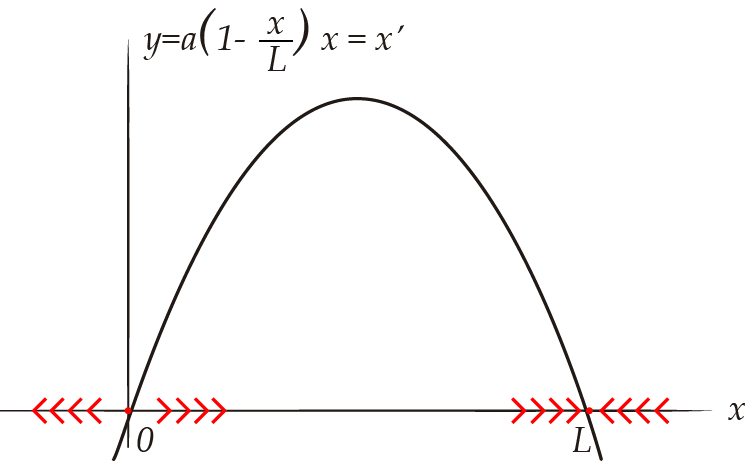
\includegraphics{1-limiterecursos.png}\label{img:1-limiterecursos}
    \end{center}
    Es fácil ver que $\mbf{x'}$ es una parábola, que corta al eje X en $0$ y $L$. Además, se indica con (>>) la dirección en la que se mueve $x(t)$ conforme avanza $t$. Tanto $0$ como $L$ son puntos de equilibrio, repulsor (inestable) y atractor (estable) respectivamente.
\end{eg}
\break

\begin{wrapfigure}{r}{0.5\textwidth}
  \begin{center}
    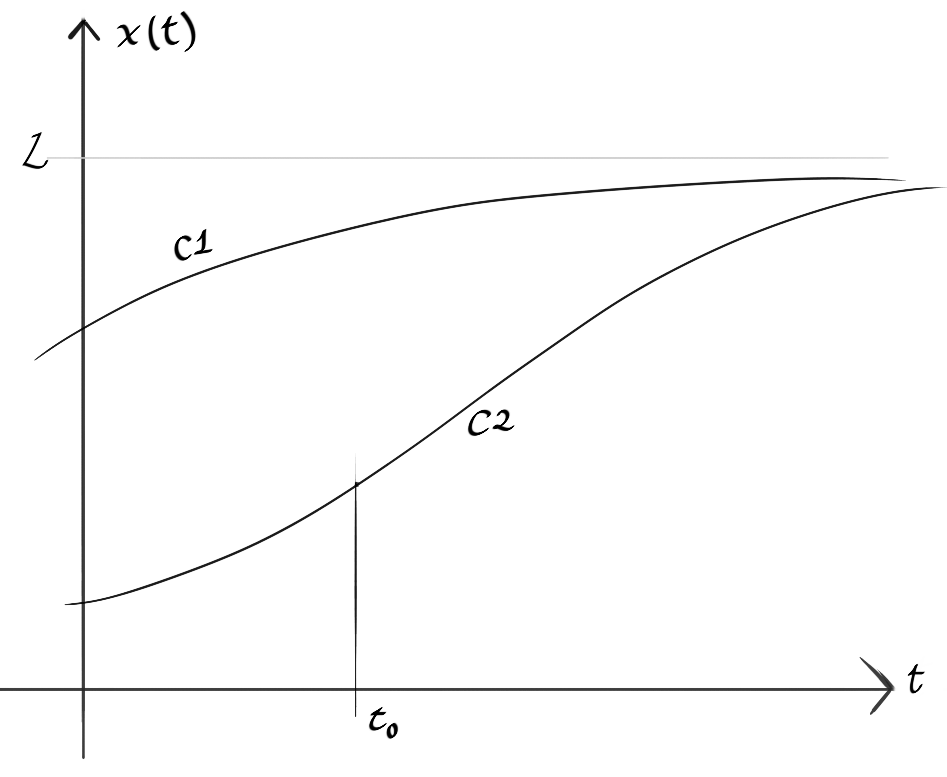
\includegraphics[width=0.48\textwidth]{1-poblaciontiempo.png}
  \end{center}
  \caption{Población - Tiempo}\label{img:1-poblaciontiempo}
\end{wrapfigure}
Habiendo encontrado las soluciones de la funcion anterior, nos preguntamos como varía la población frente al tiempo. Más adelante veremos formalmente como representar $\mbf{x}$ frente a $t$. Sin embargo, podemos razonar el aspecto de la función.
Sabemos que tiene que corregirse cerca de L, y que si $\mbf{x} << L$ entonces tiene un crecimiento parecido al exponencial. Por tanto, podría tener el aspecto de la figura \ref{img:1-poblaciontiempo}.
De este gráfico podemos deducir varias cosas. Para empezar, sabemos que $\mbf{x''}(t_0)=0$ tiene solución para la curva $c_2$ ya que tiene un punto de inflexión. Además, observamos disintos tipos de crecimiento en función del valor de $x(0)$ por lo que tendría sentido intentar determinar para qué valores $x_0$ obtenemos el crecimiento de $c_1$ y para cuáles el de $c_2$.

\begin{th_ex}\label{thex:29/01-0}
    ¿Para qué valores de $x_0$ se dan los diferentes crecimientos de $c_1$ y $c_2$?.\\
    \textit{Sugerencia}: Considerar el problema de valor inicial con $x''(t_0) = 0$.
\end{th_ex}

\section{Método de separación de variables}
Esta sección trata sobre el primer método de resolución de ecuaciones diferenciales. Antes de definir el método formalmente vamos a ver un ejemplo.
\begin{eg}[Resolución sencilla]
    Sea $\P \equiv \mbf{y'} = x\mbf{y}$. Halla las soluciones de la ecuación.\\
    $\mbf{y'} = \dd{y}{x}$, con esta igualdad podemos hacer manipulaciones sin justificar (de momento).
    $$
        \dd{y}{x} = x \mbf{y} \implies \frac{dy}{\mbf{y}} = x\mathrm{d}x \implies \int \frac{dy}{\mbf{y}} = \int x\mathrm{d}x \implies \log|\mbf{y}| = \frac{x^2}{2} + C \implies |\mbf{y}| = e^{\sfrac{x^2}{2} + C} = e^C \cdot e^{\sfrac{x^2}{2}}
    $$
    $$
        \mbf{y} = \pm e^C \cdot e^{\sfrac{x^2}{2}} = ke^{\sfrac{x^2}{2}} \mid k \in \R
    $$
\end{eg}
Esta resolución se conoce como método de separación de variables.
\begin{th_ex}\label{thex:29/01-1}
    Resolver $\P \equiv \mbf{x'} = a(1-\sfrac{\mbf{x}}{L})\mbf{x}$ con $x(0)=0$.\\
\end{th_ex}
Vamos a generalizar el método por medio de la siguiente proposición.
\begin{pro}[Método de separación de variables]
    Sea $F(x)$ una primitiva de $f(x)$ y $G(\mbf{y})$ una primitiva de $g(\mbf{y})$, es decir, $\dd{F}{x} = f(x)$ y $\dd{G}{\mbf{y}} = g(\mbf{y})$, con $\mbf{y} = f(x)$. Y sea una ecuación $\P \equiv \dd{y}{x} = \frac{f(x)}{g(\mbf{y})}$, entonces las soluciones de $\P$ cumplen:
    $$
        G(y(x)) = F(x) + \mathcal{C} \mid \mathcal{C}\ constante.
    $$
\end{pro}

\begin{proof}
    \begin{align*}
        \intertext{Por la regla de la cadena:}
            &\Dd{x} G(y(x)) = \dd{G}{\mbf{y}}(y(x)) \cdot \dd{y}{x}(x) \\
        \intertext{Como $\dd{G}{\mbf{y}} = g(\mbf{y})$ y $\dd{y}{x} = \frac{f(x)}{g(\mbf{y})}$   por hipóstesis:}
            &\dd{G}{\mbf{y}}(y(x)) \cdot \dd{y}{x}(x) = g(y(x)) \cdot \frac{f(x)}{g(y(x))} = f(x) = \Dd{x} F(x)
        \intertext{Es decir:}
            &\Dd{x}G(y(x)) = \Dd{x}F(x) \implies \Dd{x}G(y(x)) - \Dd{x}F(x) = 0 \implies G(y(x)) - F(x)  =  \mathcal{C} \implies G(y(x)) = F(x) + \mathcal{C}
    \end{align*}
\end{proof}
\begin{obs}
    La prosposición anterior está incompleta, faltaría ver que condiciones tienen que cumplir $f(x)$ y $g(\mbf{y})$. Para completarla tenemos que considerar la existencia de primitivas y la condición de que $\mathcal{C}$ sea constante.
    \begin{itemize}
        \item Ya que tenemos que usar que $F(x)$ y $G(\mbf{y})$ son primitivas, basta pedir que tanto $f(x)$ y $g(\mbf{y})$ sean continuas. Esto garantiza que $F(x)$ y $G(\mbf{y})$ son ambas $C^1$
        \item Si $h'(x) = 0 \implies h(x)$ constante en cada intervalo en que está definida (pues $\R$ es conexo). Si $h:\R \rightarrow \R$ entonces $h(x)$ es constante. Como $\mathcal{C}$ surge de integrar $0$ a la derecha de la ecuación, podemos afirmar que $\mathcal{C} = h(x)$ y por tanto constante.
    \end{itemize}
\end{obs}
\section{Significado geométrico de la ecuación diferencial ordinaria}
Vamos a analizar una ecuación diferencial de forma gráfica para interpretarla geométricamente. Consideramos $\mbf{y'} = f(x, \mbf(y))$. Supongamos que $\mbf{y}$ tiene la gráfica de la figura \ref{img:1-siggeom}.
\begin{figure}[h]
\begin{subfigure}{.5\textwidth}
    \centering
    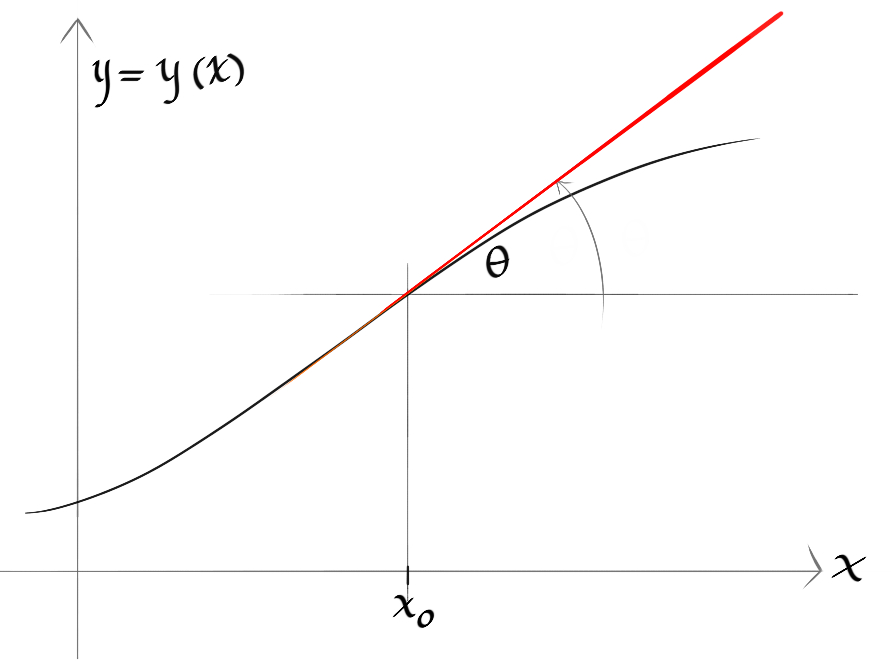
\includegraphics[width=1\textwidth]{1-significadogeom.png}
    \caption{Recta tangente en $x_0$ conocidas $\mbf{y}$ y $x_0$}\label{img:1-siggeom}
\end{subfigure}
\begin{subfigure}{.5\textwidth}
    \centering
    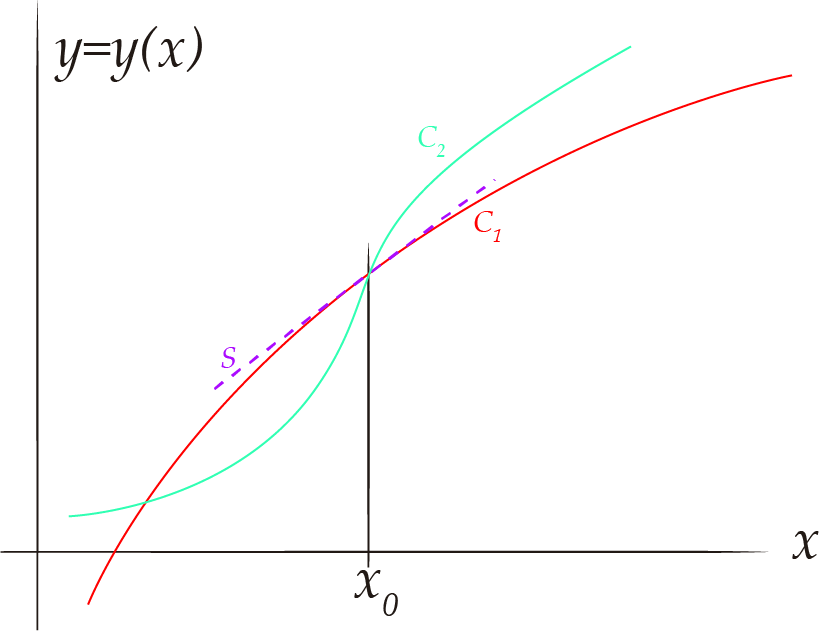
\includegraphics[width=1\textwidth]{1-significadogeom2.png}
    \caption{Curvas dadas el segmento $\mathcal{S}$.}\label{img:1-siggeom2}
\end{subfigure}
\end{figure}
Entonces, $\mbf{y'}(x_0) = \tan{\theta}$, que es la pendiente de la recta tangente a la gráfica de $\mbf{y}$ en $x_0$. Esto es cálculo elemental, lo que nos interesa es saber algo de la función $\mbf{y}$ cuando sabemos algo de $\mbf{y'}$.\\

Ilustramos en la figura \ref{img:1-siggeom2} entonces la casuística de conocer $\P \equiv \mbf{y'} = f(x,\mbf{y})$. En este caso, nos preguntamos que aspecto podría tener $\mbf{y}$ para que fuera solución de $\P$. Como conocemos $y'(x_0)$, podemos considerar que $\mathcal{S}$ es un semento paralelo a la recta tangente de la gráfica en $x_0$. Es fácil ver que $\mathcal{C}_1$ no puede ser solución de $\P$ pues $\mathcal{C}'_1(x_0) \neq y'(x_0)$. Sin embargo, es evidente que $\mathcal{C}_2$ sí resuelve $\P$.\\\\
Si repetimos el procedimiento de determinar como son las pendientes (como acabamos de hacer para $x_0$) para todos los puntos, hallamos el \textit{campo de pendientes}.

\begin{eg}[Hallar un campo de pendientes]
    Sea $\P \equiv \mbf{x'} = t^2 + \mbf{x}^2$, es decir, $f(t, \mbf{x}) = t^2 + \mbf{x}^2$. Si queremos hallar qué pendiente se le asigna al punto $p = (\sfrac{1}{\sqrt{2}},\sfrac{1}{\sqrt{2}})$ evaluamos la función $f$, $f(p) = 1$. Por tanto, la función $\mbf{x}$ que soluciona $\P$ tiene tangente con pendiente $1$ en $t = \sfrac{1}{\sqrt{2}}$.\\\\
    De hecho, es lógico pensar que a cualquier punto que cumpla $t^2 + \mbf{x}^2 = 1$ se le asignará una pendiente de $1$ a su recta tangente. Este conjunto de puntos conforman la \textbf{isoclina} de pendiente 1.\\\\
    De forma general, para una constante $c$ dada (en este ejemplo necesariamente no negativa pues $f(t, \mbf{x})$ es suma de cuadrados), podemos definir la isoclina de pendiente c:
    $$
    ISO_c = \left\{(t, \mbf{x}) \mid f(t, \mbf{x}) = c\right\}
    $$
    Volviendo a nuestro ejemplo, las isoclinas van a ser curvas que cumplan $t^2 + \mbf{x}^2 = c$ para un $c$ dado.\\
    \begin{minipage}[c]{0.3\linewidth}
      \begin{center}
          \raisebox{\dimexpr \topskip-\height}{
        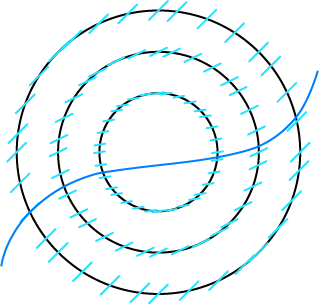
\includegraphics[width=\textwidth]{1-isoclinas.png}}
      \end{center}
    \end{minipage}\hfill
    \begin{minipage}[c]{0.65\textwidth}
        Hemos representado las isoclinas junto con un pequeño segmento de pendiente $c$ para disintos valores de $c$. Como las isoclinas cumplen que $t^2 + \mbf{x}^2 = c$, estas son las circumferencias de radio $\sqrt{c}$ con $c > 0$.\\
        Podemos observar tambien que $ISO_0 = \{(0,0)\}$ e $ISO_{c < 0} = \varnothing$.\\\\ Llamamos a la gráfica con pequeños segmentos \textit{campo de pendientes} y por tanto, una función que resuelva $\P$ tiene que ser tangente al segmento del punto por el que pase.
    \end{minipage}
    Sin embargo, los campos de pendientes permiten ver cómo es la función a grandes rasgos. En nuestro ejemplo parece indicar que $x(t) \uparrow \infty$, pero no sabemos si lo hace de forma asintótica ($x(t) \uparrow \infty$ en t finito), o x(t) crece a infinito cuando $t \rightarrow \infty$.\\
    Esto no puede resolverse gráficamente y veremos como resolverlo de forma analítica más adelante.
\end{eg}

\section{Ecuaciones diferenciales y problemas geométricos}
Gracias a la relación de la derivada con la tangencia de funciones, podemos plantear problemas geométricos en forma de ecuación diferencial.
\subsection{Trayectorias ortogonales}
De la recta tagente a un punto surge el concepto de recta normal a ese punto, que no es más que la recta perpendicular a la tangente y que pasa por dicho punto. Para ver como se relacionan estas dos rectas vamos a hacer un análisis simple. Diremos que dos curvas son ortogonales si en el punto de cruce las rectas tangentes a cada curva son perpendiculares entre sí.
\begin{wrapfigure}[20]{l}{0.5\textwidth}
  \begin{center}
    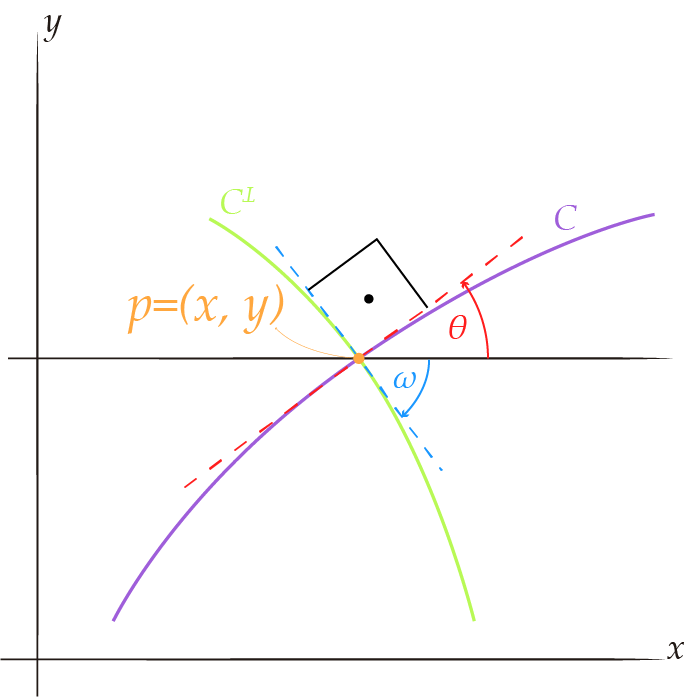
\includegraphics[width=0.48\textwidth]{1-trayectoriasortogonales.png}
  \end{center}
  \caption{Relaciones entre curvas ortogonales}\label{img:1-trayort}
\end{wrapfigure}
De la figura \ref{img:1-trayort} vemos que la pendiente de $C$ es $pend_C = \tan(\theta)$. Asimismo, $pend_{C^{\perp}} = \tan(\omega)$ y $\omega = \theta - \sfrac{\pi}{2}$. A partir de aquí desarrollamos:
$$
    \tan(\omega)=\frac{\sin(\theta-\sfrac{\pi}{2})}{\cos(\theta-\sfrac{\pi}{2})} = \frac{-\cos(\theta)}{\sin(\theta)} = -\frac{1}{\tan(\theta)}
$$
y por tanto,
\begin{equation} \label{eq:pendientes}
    pend_C \cdot pend_{C^{\perp}} = -1
\end{equation}

Nuestro objetivo es que dada una familia de curvas $fam_{C}$, podamos encontrar una (\textit{familia de}) curva que sea ortogonal a todas las de la familia en los puntos de cruce.\\\\
Supongamos que la familia original satisface una ecuación diferencial ordinaria $\mbf{y_1'} = f(x, \mbf{y_1})$. Queremos encontrar otra ecuación que defina a la ortogonal.\\\\
Como $fam_{C}$ sigue una EDO (\textit{ecuacion diferencial ordinaria}), podemos afirmar que $pend_{C} = \mbf{y_1'} = f(x, \mbf{y_1})$. Usando \ref{eq:pendientes}, $pend_{C^\perp} = \frac{-1}{f(x, \mbf{y_1})}$. Pero además, si $C^\perp$ sigue una EDO, está dada por una función $\mbf{y_2} = y_2(x)$ y entonces $\mbf{y_2'} = \frac{-1}{f(x, \mbf{y_1})}$.\\
Concluimos con que dada $fam_C$ descrita por $\mbf{y'}=f(x,\mbf{y})$, podemos encontrar $fam_{C^\perp}$ que satisface:
$$
    \mbf{y'} = -\frac{1}{f(x, \mbf{y})}
$$
\begin{eg}[Familia ortogonal a otra dada]
    Consideramos la familia: $x^2-\mbf{y}^2 = c \mid c \neq 0$\\
    Para cada $c$, eso define $\mbf{y}$ implícitamente en función de $x$.
    \begin{center}
        \vspace{1mm}
        \hfill
        \begin{tikzpicture}
            \begin{axis}[domain=-5:5,samples=150,
            restrict y to domain=-5:5,
            xtick=\empty,ytick=\empty,
            %extra x ticks={0.8,1.4}, linea vertical
            %extra y ticks=3.333333,extra y tick labels={$\frac{10}{3}$}, linea horizontal
            grid=both,axis lines=middle, axis equal
            ]
                \addplot+[no marks, thick, red, solid] ({x},{x}) node[pos=0.1, below, sloped] {$c=0$};
                \addplot+[no marks, thick, red, solid] ({x},{-x});
                %%%%%%%%%%%%%%%%%%%%%%%%%%%%%%%%%%%%%%%%%%%%%%%%%%%%%%%%%%%%%%%%%%%
                \addplot+[no marks, thick, coolblack, solid] ({(x^2+1)^(1/2)},{x}) node[pos=0.5, right] {$c > 0$};
                \addplot+[no marks, thick, coolblack, solid] ({-(x^2+1)^(1/2)},{x});
                \addplot+[no marks, thick, coolblack, densely dashed] ({(x^2+4)^(1/2)},{x});
                \addplot+[no marks, thick, coolblack, densely dashed] ({-(x^2+4)^(1/2)},{x});
                \addplot+[no marks, thick, coolblack, densely dotted] ({(x^2+9)^(1/2)},{x});
                \addplot+[no marks, thick, coolblack, densely dotted] ({-(x^2+9)^(1/2)},{x});
                %%%%%%%%%%%%%%%%%%%%%%%%%%%%%%%%%%%%%%%%%%%%%%%%%%%%%%%%%%%%%%%%%%%
                \addplot+[no marks, thick, black, solid] {(x^2+1)^(1/2)} node[pos=0.5, above, sloped] {$c < 0$};
                \addplot+[no marks, thick, black, solid] {-(x^2+1)^(1/2)};
                \addplot+[no marks, thick, black, densely dashed] {(x^2+4)^(1/2)};
                \addplot+[no marks, thick, black, densely dashed] {-(x^2+4)^(1/2)};
                \addplot+[no marks, thick, black, densely dotted] {(x^2+9)^(1/2)};
                \addplot+[no marks, thick, black, densely dotted] {-(x^2+9)^(1/2)};
            \end{axis}
        \end{tikzpicture}\hfill \break
        \vspace{1pt}
        $x^2-y^2=c$ para distintos valores de $c$.\\
        (También puede verse como las curvas de nivel del paraboloide hiperbólico)
    \end{center}
    \vspace{5pt}
    Para hallar la familia de curvas ortogonales vamos a seguir una serie de pasos:
    \begin{enumerate}
        \item \texttt{Encontrar una EDO que cumplan esas curvas.}\\
            $$
                x^2-\mbf{y}^2 = c \rightarrow \Dd{x} (x^2-y^2=c) \rightarrow 2x - 2\mbf{y}\mbf{y'} = 0 \implies \mbf{y'} = \frac{x}{\mbf{y}} = f(x,\mbf{y})
            $$
        \item \texttt{Econtrar la EDO para trayectorias ortogonales.}\\
            $$
                \mbf{y'} = -\frac{1}{f(x, \mbf{y})} = -\frac{\mbf{y}}{x}
            $$
        \item \texttt{Resolver la ecuación anterior}\\
            $$
                \dd{y}{x} = -\frac{\mbf{y}}{x} \implies -\frac{\mathrm{d}y}{\mbf{y}} = \frac{\mathrm{d}x}{x} \implies \log|y| = \log|x| + \mathcal{C}
            $$
            es decir,
            $$
                |\mbf{y}| = \frac{e^\mathcal{C}}{|x|} \implies |x\mbf{y}| = e^\mathcal{C} \implies x\mbf{y} = k : k = e^\mathcal{C} \lor k = e^{-\mathcal{C}} \implies \mbf{y} = \frac{k}{x}
            $$
    \end{enumerate}
    Con la solución general podemos representar parte de la familia:
    \begin{center}
        \vspace{1mm}
        \hfill
        \begin{tikzpicture}
            \begin{axis}[domain=-5:5,samples=150,
            restrict y to domain=-5:5,
            xtick=\empty,ytick=\empty,
            %extra x ticks={0.8,1.4}, linea vertical
            %extra y ticks=3.333333,extra y tick labels={$\frac{10}{3}$}, linea horizontal
            grid=both,axis lines=middle, axis equal
            ]
                \addplot+[no marks, very thin, black, solid] ({(x^2+1)^(1/2)},{x});
                \addplot+[no marks, very thin, black, solid] ({-(x^2+1)^(1/2)},{x});
                \addplot+[no marks, very thin, black, solid] ({(x^2+4)^(1/2)},{x});
                \addplot+[no marks, very thin, black, solid] ({-(x^2+4)^(1/2)},{x});
                \addplot+[no marks, very thin, black, solid] ({(x^2+9)^(1/2)},{x});
                \addplot+[no marks, very thin, black, solid] ({-(x^2+9)^(1/2)},{x});
                %%%%%%%%%%%%%%%%%%%%%%%%%%%%%%%%%%%%%%%%%%%%%%%%%%%%%%%%%%%%%%%%%%%
                \addplot+[no marks, thick, blue, solid, samples=500] {1/x};
                \addplot+[no marks, thick, blue, solid, samples=500] {-1/x};
                \addplot+[no marks, thick, blue, solid, samples=300] {4/x};
                \addplot+[no marks, thick, blue, solid, samples=300] {-4/x};
                \addplot+[no marks, thick, blue, solid] {9/x};
                \addplot+[no marks, thick, blue, solid] {-9/x};
            \end{axis}
        \end{tikzpicture}\hfill \break
        \vspace{1pt}
        En azul posibles soluciones para disintos valores de $k$, en negro la familia original\\
        Se observa que son curvas ortogonales a la familia original.
    \end{center}
\end{eg}

% !TeX root = ../ecuaciones-diferenciales.tex

\chapter{Integraci\'{o}n elemental}
\section{Ecuaciones homog\'{e}neas de grado 0}
En esta sección daremos un breve método para resolver ecuaciones homogéneas de grado $0$.
\begin{dfn}[Ecuación homogénea de grado k]
    Sea $f: \matbb{K} x \matbb{K} \longrightarrow \matbb{K}$, decimos que es \textbf{homogénea de grado k} $\iff f(\lambda x_1, \lambda x_2) = \lambda^k \cdot f(x_1, x_2)$
\end{dfn}
Nos interesarán especialmente las de grado $k=0$, es decir, aquellas en que $f(\lambda x_1, \lambda x_2) = f(x_1, x_2)$.\\\\
Supongamos que tenemos la EDO $\mbf{y'} = f(x, \mbf{y})$, tenemos que $f(x, \mbf{y}) = f(x, \mbf{y} \cdot \sfrac{x}{x})$. Si $f$ es homogénea de grado 0, y tomamos $\lambda = x$ entonces, $f(x, \mbf{y} \cdot \sfrac{x}{x}) = f(\lambda, y \cdot \sfrac{\lambda}{x}) = \lambda^0 f(1, \sfrac{\mbf{y}}{x})$, es decir:
$$
    \mbf{y}' = f(x,\mbf{y}) = f\left(1, \frac{\mbf{y}}{x}\right)
$$
Haciendo el cambio $\mbf{z} = \sfrac{\mbf{y}}{x}$ y desarrollando $\mbf{z'}$ tenemos:
$$
    \mbf{z'} = \frac{\mbf{y'}}{x} - \frac{\mbf{y}}{x} = \frac{f\left(1,\frac{\mbf{y}}{x}\right)}{x} - \frac{1}{x} \frac{\mbf{y}}{x} = \frac{f(1,\mbf{z}) - \mbf{z}}{x}
$$
que es una EDO de variables separables.\\Veamos un ejemplo con resolución por este método:
\begin{eg}[Espejo parabólico]
    Queremos construir un espejo para los faros de un automóvil. Buscamos que si la luz proviene del origen (la bombilla), ésta salga reflejada paralela al suelo. Vamos a hallar qué forma tiene que tener una sección del espejo (que tiene simetría radial) que cumple nuestro objetivo. Vamos a ejemplificar con la ayuda del diagrama siguiente.\\
    \begin{minipage}[c]{0.5\linewidth}
      \begin{center}
          \raisebox{\dimexpr \topskip-\height}{
        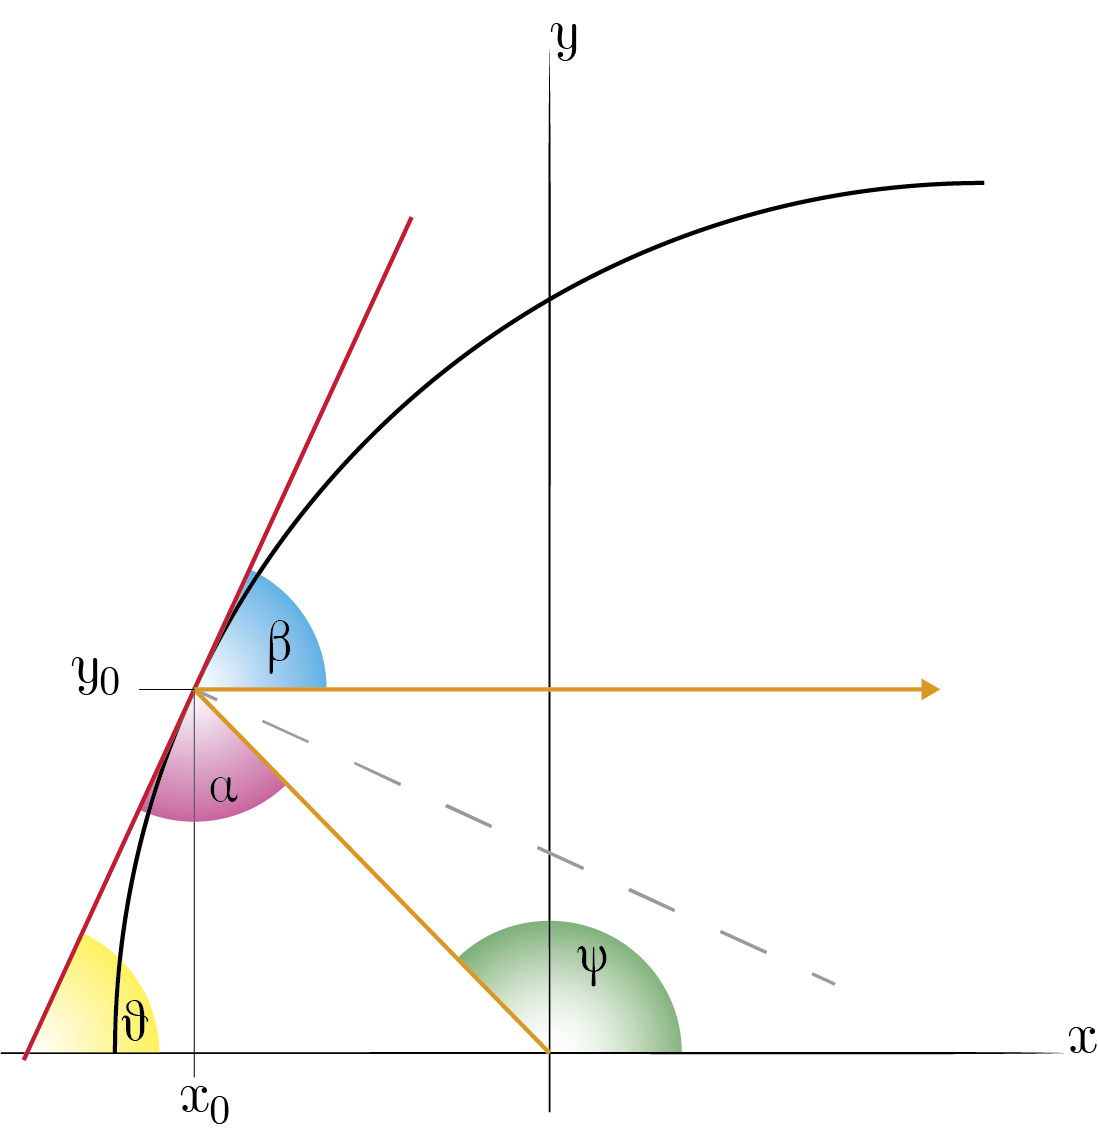
\includegraphics[width=\textwidth]{1-espejo.png}}
      \end{center}
    \end{minipage}\hfill
    \begin{minipage}[c]{0.45\textwidth}
        En la figura hemos marcado 4 ángulos: $\alpha$, $\beta$, $\theta$ y $\psi$.\\ Si nos fijamos con más detenimiento, como la trayectoria del rayo es paralela al eje $X$ los ángulos que forman ambas con la recta tangente en un punto arbitrario del espejo son idénticos, por lo que $\beta = \theta$.\\ Además, debido a que en la reflexión de un haz de luz el ángulo de reflexión coincide con el de incidencia tenemos que $\alpha = \beta$.\\ Es fácil ver que el ángulo suplementario a $\psi$ ($\pi - \psi\ rad$) forma parte de los ángulos internos de un triángulo, junto con $\alpha$ y $\theta$. Por ello, podemos expresar la igualdad $\alpha + \theta + (\pi - \psi) = \pi\ rad \implies \psi = \alpha + \theta = 2\theta$.
    \end{minipage}
    Como ya viene siendo conocido, $\tan(\theta) = \mbf{y}'$. Y si nos fijamos en la figura, para cualquier punto $(x,\mbf{y})$ del espejo $\tan(\psi) = \sfrac{\mbf{y}}{x}$. Por tanto:
    $$
        \frac{\mbf{y}}{x} = \tan(\psi) = \tan(2\theta) = \frac{\sin(2\theta)}{\cos(2\theta)} = \frac{2\sin(\theta)\cos(\theta)}{\cos^2(\theta)-\sin^2(\theta)} = \frac{2\tan(\theta)}{1-\tan^2(\theta)} = \frac{2\mbf{y'}}{1-\mbf{y'}^2}
    $$
    es decir,
    $$
        (1-\mbf{y'}^2)\cdot \mbf{y} = 2\mbf{y'}\cdot x \implies \mbf{y'} = \frac{-x \pm (x^2+\mbf{y}^2)^{\sfrac{1}{2}}}{\mbf{y}}
    $$
    de las dos opciones que tenemos, tenemos que ver cuál es válida. Como la pendiente de la recta tangente es positiva, nuestra ecuación diferencial sólo puede ser:
    $$
        \mbf{y'} = \frac{-x + \sqrt{(x^2+\mbf{y}^2)}}{\mbf{y}}
    $$
    Salta a la vista que no podemos resolverla por el método de separación de variables. Por ello, vamos a considerar un cambio de variables para convertirla en una ecuación de variables separables.\\\\
    Sea $z(x) = \sfrac{y(x)}{x}$, hallamos la expresión de $\mbf{z'}$:
    $$
        \mbf{z'} = \frac{\mbf{y'}}{x} - \frac{\mbf{y}}{x^2} = \frac{1}{x} \cdot (\mbf{y'} - \mbf{z}) = \frac{1}{x} \cdot \left(\frac{-x + \sqrt{(x^2+\mbf{y}^2)}}{\mbf{y}} - \mbf{z}\right) = \frac{1}{x} \cdot \left(-\frac{x}{\mbf{y}} +\sqrt{\left(\frac{x}{\mbf{y}}\right)^2+1} -\mbf{z}\right)
    $$
    y si del último paso hacemos el cambio $\sfrac{1}{\mbf{z}} = \sfrac{x}{\mbf{y}}$ obtenemos:
    $$
        \mbf{z'} = \frac{1}{x} \cdot \left(-\frac{1}{\mbf{z}} + \sqrt{\frac{1}{\mbf{z}^2}+1} - \mbf{z} \right)
    $$
    que es de variables separables.\\\\
    La solución a esta EDO es: $1 - \sqrt{1+\mbf{z}^2} = \frac{c}{x}$ y como $\mbf{z} = \sfrac{\mbf{y}}{x}$ obtenemos la ecuación que describe la altura de nuestro espejo en función de $x$ y una constante $c$, a falta de algún dato extra para resolver un PVI.
    $$
        y(x) = \sqrt{c^2 + 2cx}
    $$
\end{eg}

\section{Ecuaciones lineales de orden I}
Vamos a ver un nuevo tipo de ecuaciones que no se pueden resolver por los métodos anteriormente descritos, sin embargo, vamos a comenzar ejemplificando el tipo de ecuación para enunciar una proposición más adelante.

\begin{eg}[Ecuaciones lineales de orden I - Intuición]\label{eg:lineal-order}
    Sea $\mathcal{(EC)} \equiv \mbf{x'} = \mbf{x} + t$, vamos a intentar resolverla, es decir, queremos encontrar una expresión para x(t).\\
    \begin{enumerate}
        \item Vamos a considerar primero la ecuación sin el término que únicamente depende de $t$ : $\mbf{x}' = \mbf{x}$. En este caso es sencillo ver que $e^t$ es solución.

        \item Consideramos ahora $y(t) = e^{-t}x(t)$, donde $x(t)$ es solución de $\mathcal{(EC)}$ (como observación, $e^-t$ es la inversa de la solución encontrada en (1)). Derivando se obtiene que:
        $$
            y'(t) = -e^{-t}\cdot \mbf{x} + e^{-t} \cdot \mbf{x'} = e^{-t} \cdot (\mbf{x'}  - \mbf{x}) = t \cdot e^{-t}
        $$
        Solo queda integrar y despejar $x(t)$ de $y(t) = \int y'(t)$:
        $$
            y(t) = \int y'(t) \d t = \int t \cdot e^{-t} \d t = -te^{-t} - e^{-t} + C,\ C\ constante
        $$
        es decir,
        $$
            e^{-t} \cdot x(t) = -te^{-t} - e^{-t} + C \implies x(t) = Ce^t - 1 - t
        $$
    \end{enumerate}
    Con lo que hemos hallado la solución general a nuestra ecuación.
\end{eg}
\begin{obs}
    Veamos ciertos aspectos de lo que hemos hallado.\\
    \begin{enumerate}
        \item $(-1-t)$ es una solución particular de $\mathcal{(EC)}$ (cuando $C=0$).
        \item $e^t$ es solución de la \textit{ecuación homogénea} $\mbf{x'} = \mbf{x}$.
        \item Esa ecuación homogénea es lineal, es decir, la suma de ecuaciones es solución, y por tanto la multiplicación por un escalar también lo es.
        $$
        \begin{cases}
            \mbf{x'} = \mbf{x}\\ \mbf{y'} = \mbf{y}
        \end{cases}
        \implies (\mbf{x}+\mbf{y})' = \mbf{x} + \mbf{y}
        $$
        y además, si $x(t)$ es solución, $\lambda x(t)$ también lo es.
        \item Todas las solución de $\mbf{x'} = \mbf{x}$ (la homogénea) son $x(t) = Ce^t$.
        \item $x(t) = Ce^t - 1 - t$ nos dice que la solución general a $\mathcal{(EC)}$ es igual a una solución particular $(-1-t)$ más la solución de la homogénea.
    \end{enumerate}
\end{obs}
Lo que hemos hecho ha sido encontrar una solución de una ecuación del tipo $\mbf{x'} = \alpha(t)\cdot\mbf{x}+\beta(t)$ (con $\alpha(t) = 1,\ \beta(t) = t)$). Para resolver este tipo de ecuaciones enunciamos la siguiente proposición:

\begin{pro}
    Sean $\alpha,\ \beta:\ [a,b] \longrightarrow \R$ funciones continuas. Y sean:
    \begin{gather*}
        A(t) = \int_a^t \alpha(u) \d u \ \ \ \ H(t) = \int_a^t e^{-A(u)} \beta(u) \d u
    \end{gather*}
    Entonces:
    \begin{enumerate}
        \item $x(t)$ verifica $x'(t) = \alpha(t)x(t)+\beta(t)\ \forall t \in [a,b] \iff \exists c \in \R : x(t) = H(t) \cdot e^{A(t)} + c \cdot e^{A(t)}$
        \item Dados $t_0 \in (a,b)$, $x_0 \in \R$ entonces $\exists ! c : x(t) = H(t) \cdot e^{A(t)} + c \cdot e^{A(t)}$ es solución del PVI:
        $$
            \begin{cases}
                x'(t) = \alpha(t)\cdot x(t) + \beta(t)\\
                x(t_0) = x_0
            \end{cases}
        $$
    \end{enumerate}
\end{pro}
\begin{proof}
    Vamos a demostrar $1$ y $2$ por separado:
    \begin{enumerate}
        \item Tenemos $\mathcal{(EC)} \equiv x'(t) = \alpha(t)x(t) + \beta(t)$ con $\alpha, \beta$ continuas.\\
        La ecuación homogénea asociada a $\mathcal{(EC)}$ es $x'(t) = \alpha(t)x(t)$ que es lineal, es decir, la suma de soluciones es solución. Tenemos:
        $$
        \begin{cases}
            x_1'(t) = \alpha(t)x_1(t)\\
            x_2'(t) = \alpha(t)x_2(t)
        \end{cases} \implies (\mbf{x_1} + \mbf{x_2})' = \alpha(t)\cdot(\mbf{x_1} + \mbf{x_2})
        $$
        \begin{obs}
            Si sumo soluciones de $\mathcal{(EC)}$ obtengo $(\mbf{x_1} + \mbf{x_2})' = \alpha(t)\cdot(\mbf{x_1} + \mbf{x_2}) + 2\beta(t)$
        \end{obs}
        Para hallar la solución general vamos a proceder de forma parecida al ejemplo \ref{eg:lineal-order}. Sea $A(t)$ tal que $A'(t) = \alpha(t)$, entonces $x(t) = e^{A(t)}$ verifica la ecuación homogénea.\\\\
        Construimos $y(t) = e^{-A(t)}\cdot\mbf{x}$, y la igualamos con la integral de su derivada:
        $$
            (e^{-A(t)}\cdot\mbf{x})' = e^{-A}\mbf{x'} - e^{-A}\cdot \mbf{x} \cdot A' = e^{-A} \cdot (\mbf{x'} - \alpha \mbf{x}) = e^{-A} \cdot \beta
        $$
        entonces,
        $$
            y(t) = e^{-A(t)} \cdot x(t) = \int e^{-A(t)}\cdot\beta(t) \d t \implies e^{-A(t)} \cdot x(t) = H(t) + C \implies x(t) = e^{A(t)} \cdot (H(t) + C)
        $$
        \item $x_0 = x(t_0) = c\cdot e^{A(t_0)} + e^{A(t_0)} \cdot H(t) \implies \exists ! c$ pues $e^{A(t_0)} \neq 0$. Y por tanto, para el PVI:
        $$
            \begin{cases}
                x'(t) = \alpha(t)\cdot x(t) + \beta(t)\\
                x(t_0) = x_0
            \end{cases}
        $$existe solución y es única.
    \end{enumerate}
\end{proof}

\begin{eg}[Resolución ecuación lineal de orden I]
    Sea $y'(x) = x^3 - 2x\cdot y(x)$, donde $\beta(x) = x^3$ y $\alpha(x) = 2x$. Queremos hallar la expresión de todas las posibles soluciones, es decir, la solución general.\\\\
    \begin{enumerate}
        \item \texttt{Solución general de la homogénea}\\\\
        La ecuación de la homogénea es $\mbf{y}'=-2x\mbf{y}$. Es de variables separables, resolviendo obtenemos:
        $$
            y(x) = C \cdot e^{-x^2} : C \text{ es constante.}
        $$
        \item \texttt{Tomando $e^{-x^2}$ una solución de (1)}\\\\
        Volvemos a la ecuación $\mbf{y}' = x^3-2x\mbf{y}$. Por tanto, podemos reescribir $\mbf{y}' como: 2x\mbf{y} + \mbf{y}' = x^3$.\\
        A continuación, hacemos el cambio
        $$
            z(x) = e^{-(-x^2)} y(x) = e^{x^2} \mbf{y} \text{ y hallamos $z'(x)$.}
        $$
        $$
            \mbf{z}' = 2x\mbf{y}e^{x^2} + e^{x^2} = e^{x^2}\cdot (2x\mbf{y}+\mbf{y}') = e^{x^2} x^3.
        $$
        Hallamos $z(x)$ integrando $\mbf{z}'$:
        $$
            z(x) = \int x^3 e^{x^2} \d x = \frac{x^2-1}{2} \cdot e^{x^2} + C.\text{ (se resuelve por partes).}
        $$
        Igualando a nuestra $z(x) = e^{x^2} \mbf{y}$ original, despejamos $y(x)$:
        $$
            y(x) = \frac{x^2-1}{2} + C e^{-x^2}
        $$
        Donde $\frac{x^2-1}{2}$ coincide con una solución particular con $C = 0$, y $C e^{-x^2}$ es la solución general de la homogénea.
    \end{enumerate}
\end{eg}
%%Considerar si añadir la primera parte de la clase del 05/02
\section{Teoremas de existencia y unicidad}
En la sección anterior hemos enunciado una preposición que denominamos de \texit{existencia y unicidad} para ecuaciones lineales de orden I. Nos gustaría dar condiciones más generales para saber si existen y son únicas ciertas soluciones.\\
Consideraremos el PVI general:
$$
    \begin{cases}
        \mbf{x'} = f(t, \mbf{x}) \\ x(t_0) = t_0
    \end{cases}
$$
\begin{thm}[Existencia y unicidad global]
    Sea $f: [a,b] \subset \R \longrightarrow \R$, con $f \in C^1$.\\Si $\dd{f}{x} = f_x$ es acotada,  es decir:
    $$
        \exists L \in \R : |f_x(t, \mbf{x})| \leq L\ \forall t\in[a,b],\ \forall x\in R
    $$ entonces, el PVI tiene solución y es única.
\end{thm}
La demostración la veremos más adelante cuando consideremos el caso \texit{n-dimensional}.

\begin{obs}
    Vamos a ver ciertos aspectos de este resultado.\\
    \begin{enumerate}
        \item  Gráfica de la solución\\
        \begin{minipage}[c]{0.5\linewidth}
          \begin{center}
              \raisebox{\dimexpr \topskip-\height}{
            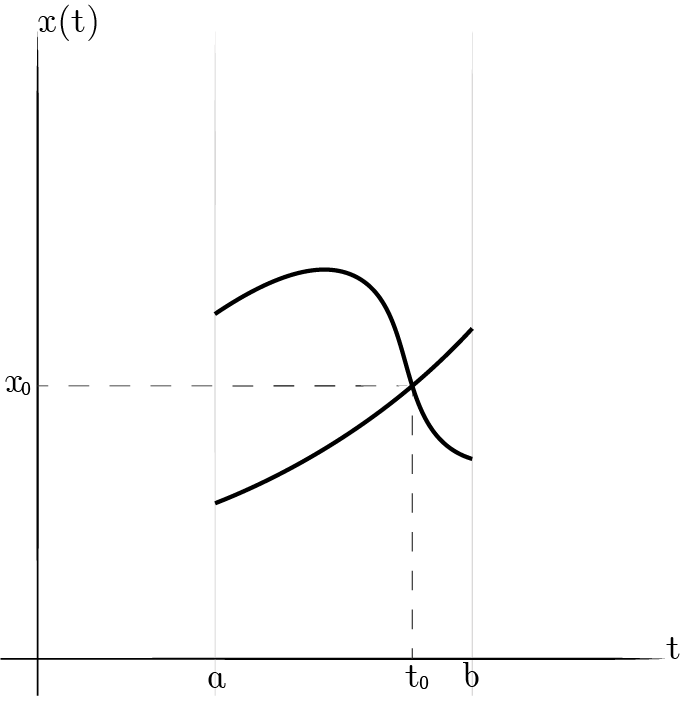
\includegraphics[width=\textwidth]{1-existencia-unicidad.png}}
          \end{center}
        \end{minipage}\hfill
        \begin{minipage}[c]{0.45\textwidth}
            A nivel visual, no puede haber dos soluciones como las de la figura. Si las hubiera, el PVI tendría dos soluciones distintas para $t_0$ y habíamos dicho que era única.\\\\
            Analíticamente podemos considerar el gráfico de $x(t)$ como un subconjunto del plano $\R^2$. Si consideramos cada solución de esta forma, digamos $S_1, S_2$, entonces:
            $$
                S_1 \cap S_2 \neq \varnothing \iff S_1 = S_2
            $$
        \end{minipage}
        \item Unicidad en la recta real\\
        \begin{minipage}[c]{0.5\linewidth}
          \begin{center}
              \raisebox{\dimexpr \topskip-\height}{
            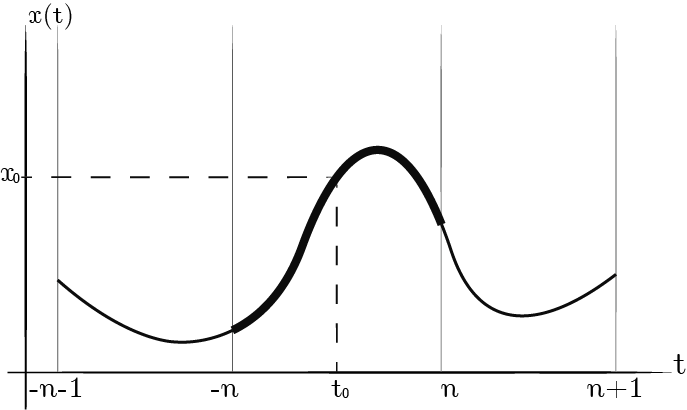
\includegraphics[width=\textwidth]{1-extension-unicidad.png}}
          \end{center}
        \end{minipage}\hfill
        \begin{minipage}[c]{0.45\textwidth}
            Sea $f: \R \times \R \longrightarrow \R$ cumple que $|f_x \leq L|$ (su derivada está acotada), entonces el PVI:
                $$
                    \begin{cases}
                        \mbf{x'} = f(t, \mbf{x})\\
                        x(t_0) = x_0
                    \end{cases}
                $$
            entonces tiene solución y es única $ \forall t \in \R$\\\\
            Si nos fijamos en la imagen de la izquierda, la idea intuitiva surge de tener una solución $x(t)$ definida sobre un intervalo $[-n, n]$. Si podemos extender $x(t)$ a $[-n-1, n+1]$, ésta tiene que coincidir en $[-n,n]$ y por unicidad, la solución es la misma. Podemos hacer esto para cualquier intervalo mayor que $[-n,n]$ y por tanto sobre la totalidad de $\R$.\\Formalmente puede intentar demostrarse por inducción sobre el tamaño del intervalo.
        \end{minipage}
        %% Mirar si introducir el ejemplo de mi página 19. Parece repetido.
    \end{enumerate}
\end{obs}
\begin{th_ex}
    Supongamos que $x(t)$ resuelve $\mbf{x'} = f(x)$ y $\lim_{t \to \infty} x(t) = a$. ¿Podemos asegurar que $f(a) = 0$?.\\ \textit{Pista:} tener en cuenta que el recíproco es cierto. Es decir, si $f(a) = 0$ entonces sabemos que hay ecuaciones que se acercan a $a$ conforme avanzan.
\end{th_ex}
La versión global del teorema de existencia y unicidad no es muy útil. Veamos dos situaciones simples en las que no funciona.\\\\
Sea el PVI:
$$
    \begin{cases}
        \mbf{x'} = \mbf{x}^2\\
        x(0)=1
    \end{cases} t\in [-2,2] \text{ no tiene solución.} \label{eg:no-solution}
$$
Si intentamos resolverlo:
\begin{gather*}
    \dd{x}{t} = \mbf{x}^2 \implies \int \frac{\d x}{\mbf{x}^2} = \int \d t \implies -\frac{1}{\mbf{x}} = t + C\\
    x(0) = 1 \implies C = -1 \implies x(t) = \frac{1}{1-t}
\end{gather*}
que no es solución en $[-2,2]$ pues no está definida para $t=1$.\\\\

\begin{wrapfigure}[12]{r}{0.6\textwidth}
  \begin{center}
    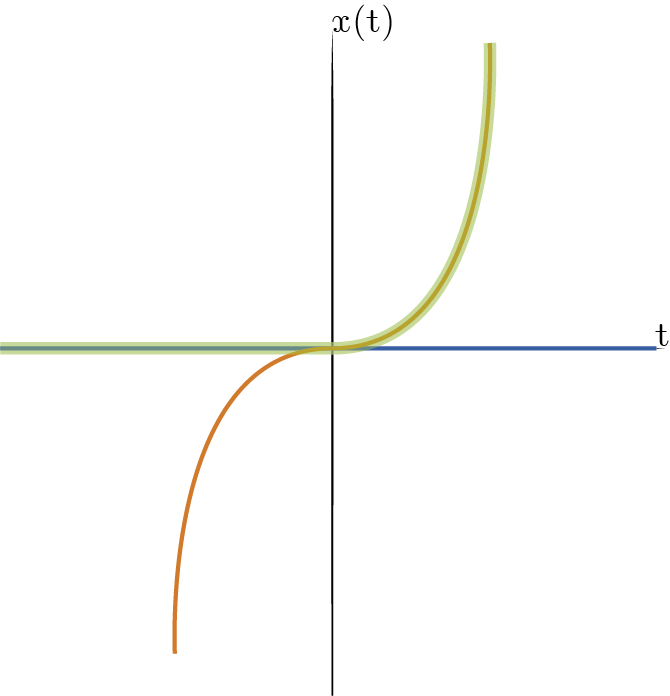
\includegraphics[width=0.4\textwidth]{1-no-unicidad.png}
  \end{center}
  \caption{Solución no única}\label{img:1-no-unicidad}
\end{wrapfigure}
Consideremos ahora el PVI:
$$
    \begin{cases}
        \mbf{x'} = \mbf{x}^{\sfrac{2}{3}}\\
        x(0)=0
    \end{cases}
$$
es fácil ver que tanto $x_1(t) = 0$ como $x_2(t)=(\frac{t}{3})^3$ resuelven el PVI. De hecho, si combino trozos de la función puedo hallar más. En la figura se representan ambas soluciones y se resalta una posible combinación.\\\\

\begin{thm}[Existencia y unicidad local]
    Sean $[a,b] \times [c,d] = A \subset \R \times \R$, una función $f: A \longrightarrow \R$ con $f \in C^1$ y $t_0\in(a,b)$, $x_0\in(c,d)$. Entonces:\\
    \begin{itemize}
        \item Existencia:\\
            $
                \exists \delta > 0 \text{ y } x:(t_0 - \delta, t_0 + \delta) \longrightarrow \R, \mbf{x}\in C^1
            $ tal que $\mbf{x}$ es solución del PVI:
            $$
                \begin{cases}
                    \mbf{x'} = f(t, \mbf{x})\\
                    x(t_0) = x_0
                \end{cases}
                \text{con } \delta < \min(t_0 - a, b - t_0)
            $$
        \item Unicidad:\\
        Si $x_1(t)$, $x_2(t)$ son $C^1$ en un intervalo $(t_0-\varepsilon, t_0+\varepsilon)$ y satisfacen:\\
        $$
            \begin{cases}
                \mbf{x_i'} = f(t, \mbf{x_i}),\ |t-t_0| < \varepsilon\\
                x_i(t_0) = x_0
            \end{cases}
            \text{con } \varepsilon < \min(t_0 - a, b - t_0)
        $$ entonces $x_1(t) = x_2(t)\ \forall t : |t-t_0| < \varepsilon$.
    \end{itemize}
\end{thm}
De nuevo, se deja la demostración para cuando enunciemos el caso \textit{n-dimensional}.
\begin{obs}
    Al igual que en el caso global, vamos a estudiar una serie de implicaciones de este resultado.\\
    \begin{enumerate}
        \item Unicidad local.\\
        Podemos expresar la solución analíticamente como:\\\\
        Sean $x_1(t),\ x_2(t)$ soluciones a un PVI. Si $x_1(t_0) = x_2(t_0)$, entonces $ \exists \varepsilon>0: x_1(t) = x_2(t),\ \forall t : |t-t_0| < \varepsilon$
        \item Prolongación de la solución.\\
        \begin{center}
            \raisebox{\dimexpr \topskip-\height}{
          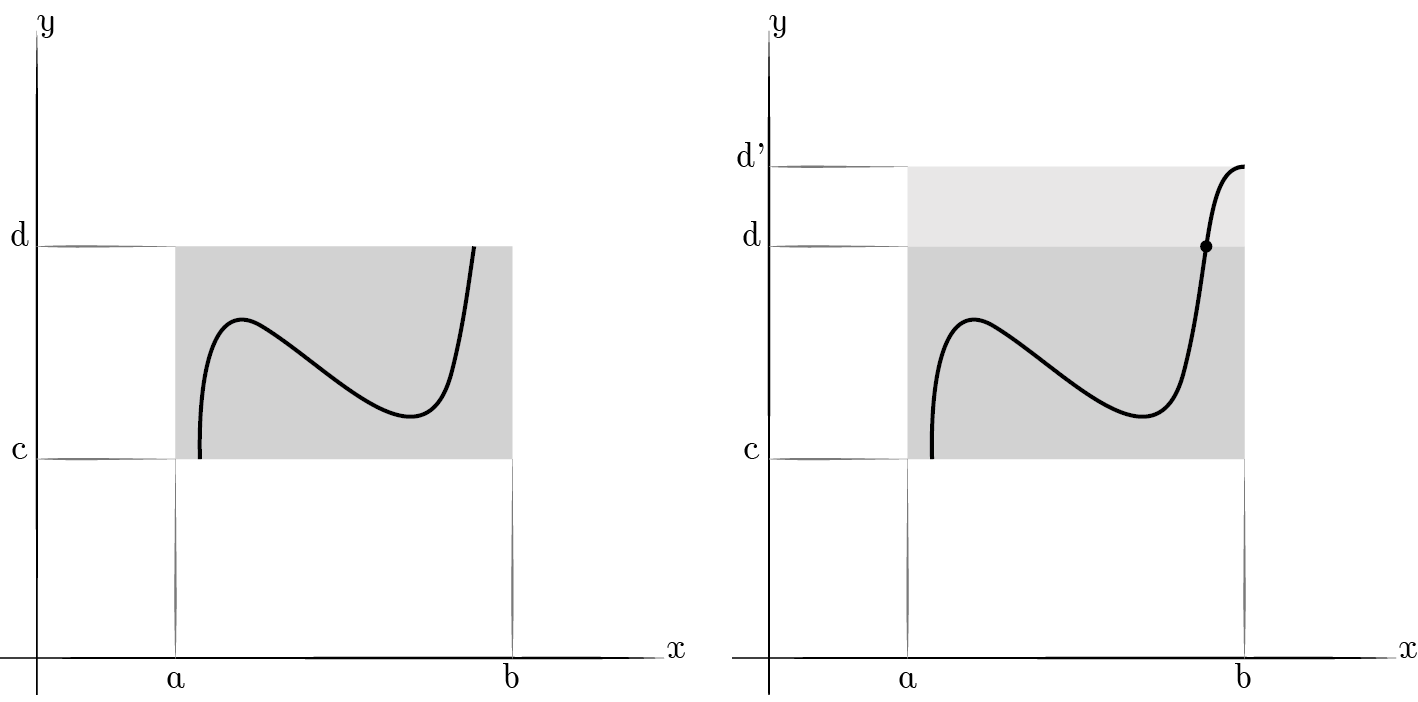
\includegraphics[width=0.7\textwidth]{1-prolongacion-solucion.png}}
        \end{center}
        Puede ocurrir que hayamos definido la función sobre un área más pequeña de lo necesario. En la imagen superior se representa esta casuística.\\
        En este caso, podemos prolongar la solución gracias a la unicidad, si existiera otra solución con $t\in[a,b]$ que estuviera definida en todo $[c, d']$, entonces debería coincidir con nuestra solución original por compartir el punto $(t, d)$. Podríamos preguntarnos  entonces si existe un intervalo cerrado máximo en el que existe nuestra solución.
        \item Acerca de las hipótesis.\\
        No es necesario pedir que $f \in C^1$. Para la existencia sólo necesitamos que $f$ sea continua, y para la unicidad nos basta con que $f_x$ exista y sea continua. En el caso general veremos que podemos pedir incluso menos para la unicidad.
    \end{enumerate}
\end{obs}

\subsection{Regularidad de soluciones}
En ocasiones nos va a interesar saber como de buena es la función que resuelve nuestra EDO, entendiendo buena por cómo de suave es. Supongamos que nuestra ecuación diferencial es $x'(t) = f(t, x(t))$ definida en un intervalo, con $f:[a,b] \times [c,d] \subset \R^2 \longrightarrow \R$ continua y $x(t)$ derivable.\\
Entonces:
\begin{align*}
    x(t) \text{ derivable} &\implies x(t) \text{ continua}.\\
    \begin{cases}
        x(t) \text{ continua}\\
        f(t_1, t_2) \text{ continua}
    \end{cases} &\implies [\text{componiendo $f$ con $x(t)$ como $t_2=x(t)$})]\ f(t, x(t))\text{ es continua}\implies\\
     &\implies x'(t)\text{ es continua}\implies x(t) \in C^1
\end{align*}
Además, si $f(t_1, t_2) \in C^1$ entonces $f(t, x(t)) \in C^1$, pues:
$$
    \Dd{t}(f(t, x(t))) = f_t(t, x(t)) + f_x(t, x(t)) \cdot x'(t)
$$
De donde sabemos que tanto $f_t$ como $f_x$ son continuas pues $f(t_1, t_2) \in C^1$ y $x'(t)$ es continua como acabamos de ver. Y como $x''(t) = \Dd{t}(x'(t)) = \Dd{t}(f(t, x(t)))$ que es continua, entonces $x(t) \in C^2$.\\\\
Repitiendo este argumento, concluimos con que: $f(t_1,t_2) \in C^k \implies x(t) \in C^{k+1}$.

\section{Ecuaciones exactas}
Hasta ahora hemos visto como resolver ecuaciones de variables separables, homogéneas de grado 0 y lineales de orden I. Veamos un método más.\\\\
Supongamos que $\mbf{y}$ está definida implícitamente por $g(x, \mbf{y}) = cte$ con $g \in C^1$. Si derivamos $g(x, \mbf{y}) = cte)$ respecto de $x$ obtenemos:
$$
    g_x(x, y(x)) + g_y(x, y(x)) \cdot y'(x) = 0, \text{ es decir,}
$$
$y(x)$ se resuelve a partir de.
$$
    \mbf{y'} = -\frac{g_x(x,\mbf{y})}{g_y(x,\mbf{y})}
$$
\begin{obs}
    Podemos argumentar a la inversa. Si $y(x)$ verifica la EDO, entonces $g(x, y(x))$ es constante (en intervalos), pues $\Dd{x}(g(x, y(x))) = 0$
\end{obs}
Además, la notación habitual para este tipo de ecuaciones es:
$$
    \mbf{y'} = \dd{y}{x} = -\frac{g_x(x,\mbf{y})}{g_y(x,\mbf{y})} \implies g_x\d x + g_y \d y = 0
$$
Supongamos que tenemos una ecuación $y'(x) = -\frac{M(x,y)}{N(x,y)}$, es decir, $M\d x + N \d y = 0$. Nos gustaría saber cuándo existe $g(x, \mbf{y}) : M = g_x,\ N = g_y$, ya que en ese caso es exacta y su solución es $g(x, \mbf{y}) = C \mid C \text{constante}$ en forma implícita.
\begin{eg}[Ecuación exacta simple]
    Sea $\mbf{y'} = \frac{-\mbf{y}}{x}$, es decir, $\mbf{y}\d x + x \d y = 0$ es una ecuación exacta.\\
    De hecho la $g$ necesaria es $g(x,\mbf{y}) = xy$ pues $g_x = \mbf{y}$ y $g_y = x$. Y por tanto, la solución general es:
    $$
        x\mbf{y} = C \implies y(x) = \frac{C}{x}
    $$
    De hecho, esta ecuación es de los tres tipos que hemos visto.
\end{eg}
\begin{pro}[Condición necesaria de ecuación exacta]
    $$
        \mathcal{EC} \equiv M\d x + N\d y \text{ es exacta y }g(x, \mbf{y}) \in C^2 \implies M_y = N_x
    $$
\end{pro}
\begin{proof}
    Si $\mathcal{EC}$ es exacta, entonces $\exists g : M = g_x,\ N = g_y$. Como $g \in C^2$, sabemos que $g_{xy} = g_{yx}$, entonces:
    $$
        \begin{cases}
            g_{xy} = (g_x)_y = M_y\\
            g_{yx} = (g_y)_x = N_x
        \end{cases} \implies M_y = N_x
    $$
\end{proof}
\begin{obs}
    Sabemos que una ecuación es exacta cuando $(M, N) = \Nabla g$, sea $\gamma$ cualquier curva tal que $\gamma : [a,b]\subset\R \longrightarrow \R^2$ en $\R^2$. Entonces:
    $$
        \int_\gamma M\d x + N\d y = g(\gamma(b)) - g(\gamma(a))
    $$
    Es claro que si la curva es cerrada, $\gamma(a)=\gamma(b)$ y la integral es nula.
\end{obs}

\begin{eg}[Ecuación exacta]
    Sea $\mathcal{(EC)} \equiv (\mbf{y}+x^3) dx + (x+\mbf{y}^3) dy = 0$ es fácil ver que cumple la condición de $M_x = N_y$.\\
    Nos gustaría hallar cual sería nuestra $g$ a partir de que $g_x=M$ y $g_y=N$. Sabemos que $g_x = M = y + x^3$.
    Si integramos en $x$ (suponiendo $\mbf{y}$ constante):
    $$
    g(x,\mbf{y} = yx + x^4/4 + C(y) \text{para C una constante vista desde $x$}.
    $$
    Además,
    \begin{gather*}
        x+\mbf{y}^3 = N = g_y = x + c'(\mbf{y}) \implies c'(\mbf{y}) = \mbf{y}^3\\
        c'(\mbf{y}) = \mbf{y}^3 \implies c(\mbf{y}) = \frac{\mbf{y}^4}{4} + cte.
    \end{gather*}

    Por lo que tenemos: $g(x,\mbf{y}) = x\mbf{y} + \frac{x^4+\mbf{y}^4}{4}$. Es decir, las soluciones de $\mathcal{(EC)}$ vienen dadas por $xy + \frac{x^4+y^4}{4} = C \text{($C$ constante)}$.\\

    Por ejemplo, una solución particular para C=1 es:

    $$xy + \frac{x^4+y^4}{4} = 1, \text{ que es la curva roja en la imagen siguiente.}$$
    \begin{center}
        \raisebox{\dimexpr \topskip-\height}{
      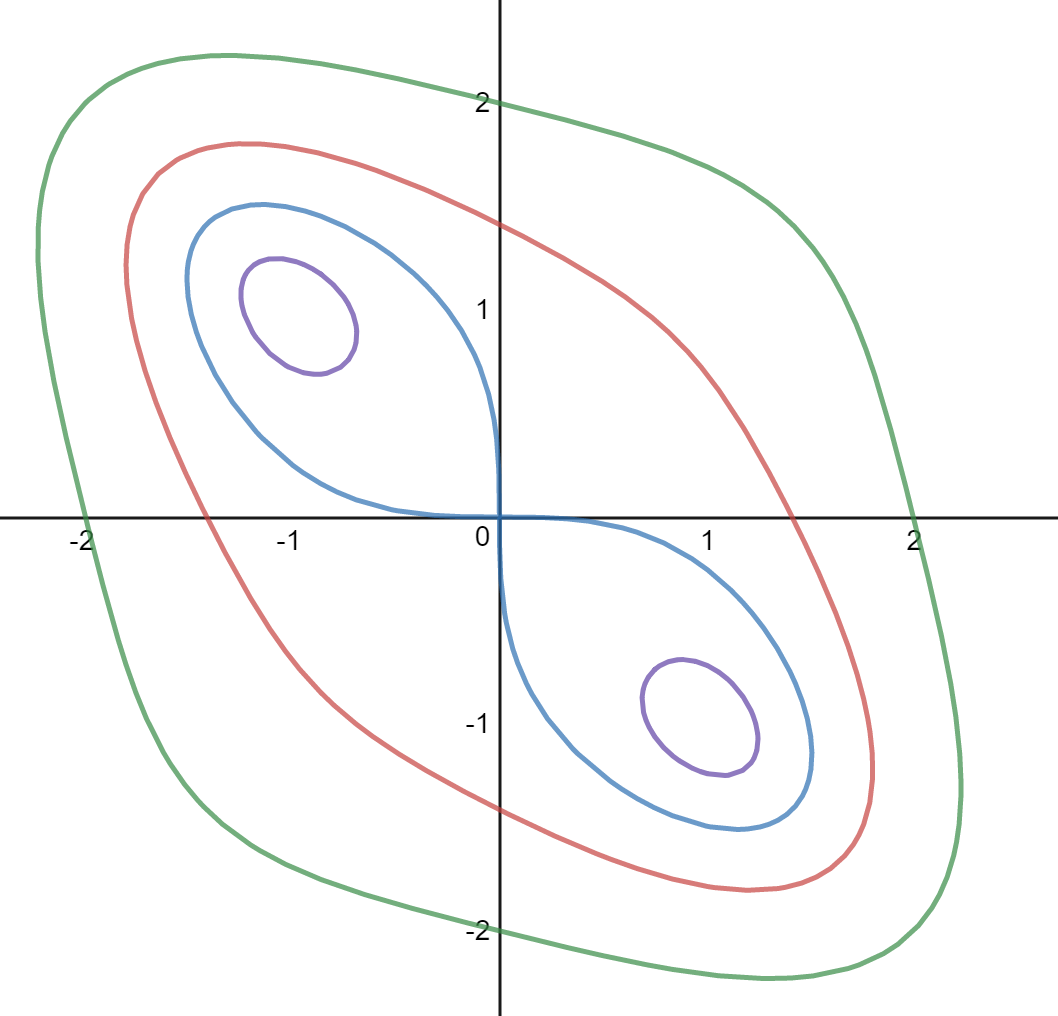
\includegraphics[width=0.5\textwidth]{1-ecuacion-exacta.png}}
    \end{center}
\end{eg}

Queremos ahora analizar la condición necesaria y suficiente que nos asegure que podamos realizar el procedimiento del ejemplo. Haremos uso de la siguiente proposición.
\begin{pro}
Sea $\Omega\subset\R^2$ un abierto simplemente conexo. Sean $M, N : \Omega \to \R\text{ con } M,N \in C^1$, entonces:
$$
\exists g : \Omega \to \R \text{ con } g \in C^2 \text{ tal que } M = \left.g_x\right|_\Omega, \left.N=g_y\right|_\Omega \iff \left.M_y\right|_\Omega = \left.N_x\right|_\Omega.
    $$
\end{pro}
La demostración se deja al lector.\\\\
A modo de recordatorio vamos a dar una definición de \textit{abierto simplemente conexo}.
\begin{dfn}[Conjunto simplemente conexo]
    Sea $\Omega \subset \R^2$ un abierto acotado.\\
    Decimos que $\Omega$ es \textbf{simplemente conexo} $\iff$ $\Omega^C = \R^2\Omega$ es conexo.
\end{dfn}

\section{Factores integrantes}
Sea de nuevo $\mathcal{(EC)}_1 = M \d x + N\d y = 0$, pero supongamos ahora que no se cumple la condición $M_x = N_y$ necesaria para encontrar una ecuación exacta. Nos preguntamos si podemos encontrar un $\mu(x, \mbf{y})$ no trivial de forma que teniendo la ecuación $\mathcal{(EC)}_2 = \mu(x, \mbf{y}) M \d x + \mu(x, \mbf{y}) N\d y = 0$ se cumpla:
\begin{equation}\label{eq:factor-integrante}
    (\mu M)_y = (\mu N)_x
\end{equation}
Llamamos a $\mu$ factor integrante de $\mathcal{(EC)}_1$. Veremos que siempre existe pero que es difícil de encontrar.\\
Calculando \ref{eq:factor-integrante}, obtenemos:
\begin{gather*}
    M \frac{\partial \mu}{\partial y} - N \frac{\partial \mu}{\partial x} + (M_y - N_x) \mu = 0\\
    \left(M \frac{\partial}{\partial y} - N \frac{\partial}{\partial x}\right)\mu + (M_y - N_x) \mu = 0
\end{gather*}
de donde tendremos que calcular $\mu$. Como suele resultar difícil, habitualmente se intenta que $\mu$ solo dependa de una de las dos variables, es decir, $\mu=\mu(y)$ o $\mu=\mu(x)$.\\\\

%%%%%%%%%%%%%%%%%%%%%%%%%%%%%%%%%%%%%%%%%%%%%%%%%%%%%%%%%%%%%%%% Clase del 11/02
Veamos un ejemplo de ecuación de factores integrantes
\begin{eg}[Factores integrantes]
    Sea $x\mbf{y}\ \d x + \mb{y}^2 \d y = 0$, esta claro que $M = x\mbf{y}$, $N = \mbf{y}^2$. Para ver si puede ser una ecuación exacta evaluamos si cumple la condición necesaria $M_y = N_x$, sin embargo las derivadas cruzadas son $M_y=x$ y $N_x = 0$ y por tanto no puede ser ecuación exacta.\\\\
    Nos preguntamos entonces por cual es su factor integrante. Para encontrarlo vamos a intentar que $\mu$ dependa solo de una variable (o de una combinación lineal, por ejemplo $z = x+y$).\\
    \begin{enumerate}
        \item \texttt{Intentamos que $\mu$ dependa de $x$.}\\\\
            Transformamos nuestra ecuación en: $(\mathcal{EC})\equiv \mu M\ \d x + \mu N\ \d y = 0$. Es decir, tenemos:
            $$
                \mu(x)\ x\mbf{y}\  \d x + \mu(x)\ \mbf{y}^2\ \d y = 0, \text{entonces hallamos las nuevas $M_y$ y $N_x$ para hallar $\mu$}
            $$
            como se tiene que cumplir que $M_y = N_x$
            $$
                M_y = \mu(x)\ x = \mu'(x)\ \mbf{y}^2 = N_x \implies \frac{\mu'(x)}{\mu(x)} = \frac{x}{\mbf{y}}
            $$
            y es claro que no tiene solución, pues la parte de la izquierda no depende de y.
        \item \texttt{Intentamos que $\mu$ dependa de $\mbf{y}$.}\\\\
        Repitiendo el mismo procedimiento, hallamos las nuevas $M_y$ y $N_x$ para hallar $\mu$ que cumple la condición necesaria. Obtenemos:\\\\
        $$
            \frac{\mu'(y)}{\mu(y)} = \frac{-1}{y} \implies (log |\mu|) = -log |y| \implies \mu(y) = \frac{1}{y} \text{ es solución}.
        $$
        Es decir, $(\mathcal{EC}) \equiv x\ \d x + \mbf{y}\ \d y = 0$. Podemos resolverla por separación de variables y su solución es:
        $$
            \frac{x^2+\mbf{y}^2}{2} = C \implies x^2+\mbf{y}^2 = C
        $$
    \end{enumerate}
\end{eg}

\begin{obs}
    Sea la ecuación lineal de primer orden $\mbf{y}' = a(x) \cdot \mbf{y} + b(x)$.\\
    Con $A(x) : A'(x) = a(x)$ $(e^{A(x)})$. %%TODO: Completar
    Entonces $e^{-A(x)}$ es un factor integrante de $y'(x) = a(x) \cdot y(x) + b(x)$.
\end{obs}

\begin{eg}[Análisis de cotas en una ecuación diferencial]
Vamos a hacer un aparte para retomar el ejemplo \ref{eg:campo-pendientes}. Teníamos que $(\mathcal{EC}1) \equiv \mbf{x}' = t^2 + \mbf{x}^2 = f(t, \mbf{x})$ y llegábamos a la conclusión a través de trazar su campo de pendientes de que $x(t) \uparrow \infty$, pero no sabíamos si lo hacía de forma asintótica o lo alcanza cuando $t \to \infty$, aunque el campo parecía indicar que lo hacía de forma asintótica en $t=1$ o antes. Vamos a tratarla de forma analítica comparándola con otra ecuación que se asemeja y que ya conocemos.\\\\
Sabemos que $|f_x| < L$ no se cumple, pues $2x \to \infty$ si $x \to \infty$ y no podemos aplicar el teorema de existencia y unicidad global.\\
Vamos a comparar la solución de $(\mathcal{EC}1)$ donde exista con la de:
$$
    (\mathcal{EC}2)\equiv
    \begin{cases}
        \mbf{x}' = \mbf{x}^2\\
        x(0) = 1
    \end{cases}
$$
Sean $u(t)$ la solución de $(\mathcal{EC}1)$ y $v(t)$ la solución de $(\mathcal{EC}2)$. A primera vista en $t=0$ ambas tienen la misma pendiente pues $f(0,1) = 1$.
Sabemos también que $u(t)$ crece más rápido que $v(t)$ por que en el momento en que $t \neq 0$, crecerá más rápido (pues $t^2 + x(t^2) \geq x(t^2)$). Cualitativamente podemos afirmar que $u(t)$ "va por encima" de $v(t)$. Nos gustaría hacer una comparativa cuantitativa de ambas.\\\\
Para ello, consideramos $z(t) = u(t) - v(t)$. Ahora, calculamos $z'(t)$:
$$
    z'(t) =  u'(t) - v'(t) = t^2+u^2-v^2 = t^2 + (u - v)\cdot(u + v) = t^2 + \mbf{z}\cdot(u + v).
$$
En este caso no conocemos explícitamente $(u(t)+v(t))$, pero podemos afirmar que como $(u(t),v(t))$ son crecientes $\forall t\geq0$ y para $t=0$ valen 1, entonces $(u + v) \geq 2$. Por tanto,
$$
    \mbf{z}' \geq 2\mbf{z} + t^2 \implies \mbf{z}' - 2\mbf{z}\geq t^2.
$$
Sea $w(t) = e^{-2t}\cdot z(t)$, entonces $\mbf{w}' = e^{-2t}(\mbf{z}'-2\mbf{z}) \geq e^{-2t}t^2 \geq t^2$. Entonces $\mbf{w}' \geq e^{-2t}t^2$ y además $w(0) = z(0) = 1 - 1 = 0$. A partir de esto tenemos:
$$ %%TODO: Preguntar por esta definición de w(t)
    w(t) = w(0) + \int_0^t w'(s) \d s \geq \int_0^t s^2 e^{-2s} \d s = \left.e^{-2s} \cdot \frac{2s^2 + 2s + 1}{4}\right|_0^t
$$
es decir,
$$
    w(t) \geq \frac{1}{4} - e^{-2t} \frac{2t^2 + 2t + 1}{4} \text{, y como } w(t) = e^{-2t} z(t) \text{ entonces,}
$$
$$
    z(t) \geq \frac{e^{2t} - (2t^2 + 2t + 1) }{4} \implies u(t) - v(t) \geq \frac{e^{2t} - (2t^2 + 2t + 1) }{4} \implies u(t) \geq v(t) + \frac{e^{2t} - (2t^2 + 2t + 1) }{4}
$$
Como vimos en \ref{eg:no-solution}, $v(t) = \frac{1}{1-t}$ y por tanto $v \to \infty$ cuando $t \to 1$. Y ya que $u(t) \geq v(t) + \frac{e^{2t} - (1 + 2t + 2t^2)}{4}$, $u \to \infty$ antes de $t = 1$.
\end{eg}
\begin{th_ex} %TODO: Que cojones es esto
    Encontrar otra ecuación que sea sencilla de resolver para $u(t) \geq x$.
\end{th_ex}

%%%%%%%%%%%%%%%%%%%%%%%%%%%%%%%%%%%%%%%%%%%%%%%%%%%%%%%%%%%%%%%% Clase del 12/02

\section{Ecuaciones reducibles de orden II}
Hasta ahora hemos estudiado distintas ecuaciones de orden I. Vamos a ver un nuevo tipo de ecuaciones que involucra la segunda derivada y hay diversos ejemplos en el estudio de la Física.

\begin{dfn}[Ecuaciones de orden II]
    Sea $\mbf{x} = f(t)$, una \textbf{ecuación diferencial de segundo orden} es una ecuación de la forma: $\mbf{x}'' = F(t, \mbf{x}, \mbf{x}')$
\end{dfn}

\begin{obs}
    La ecuación $\mbf{x}'' = 5\mbf{x}'$ es de orden 2 sólo formalmente, ya que se resuelve como una de primer orden. Con $y(t) = 5\mbf{y}, \mbf{y}' = 5\mbf{y} \implies y(t) = ce^{5t} \implies x(t) = \int C e^{5t} = a + b e^5t$. Sin embargo tenemos dos parámetros, para determinarlos necesitamos añadir dos condiciones. El PVI entonces sería del tipo:
    $$
        \begin{cases}
            \mbf{x}'' = 5\mbf{x}'\\
            x(0) = 1\\
            x'(0) = 0
        \end{cases}
    $$
    Con esto hallaríamos $a+b = 1$, $b=0$.\\\\
    Sin embargo, podemos tener otro tipo de condiciones que no serían un PVI, por ejemplo, dar dos condiciones para x(t) y ninguna para x'(t). Estas no tienen aseguradas existencia y unicidad y lo veremos más adelante.
\end{obs}

Como fuente de ejemplos para esta sección utilizaremos la segunda ley de Newton $F = m\cdot a$.

\begin{eg}[Muelles]\label{eg:muelle}
    %%TODO: Incluir dibujo del muelle.
      \begin{center}
        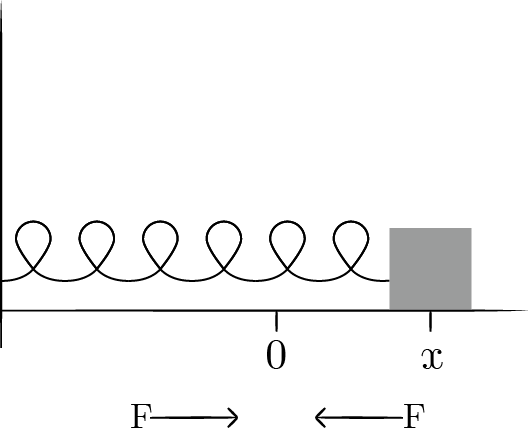
\includegraphics[height=0.1\textheight]{1-muelle.png}
      \end{center}
        Consideramos que $x=0$ corresponde a la situación de equilibrio, es decir totalmente parado. Además vamos a suponer que:
        \begin{itemize}
            \item no hay fricción con la superficie ni con el aire.
            \item tenemos movimientos oscilatorios desde la situación de equilibrio.
            \item la masa es puntual.
        \end{itemize}
        La fuerza por tanto se expresa como $F = -k x$, donde $k$ es la constante del muelle y es negativa por que va en sentido contrario al vector posición con origen en $x=0$.\\\\
        La ecuación diferencial de este modelo es:
        $$
            m\mbf{x}'' = -k \mbf{x} \implies \mbf{x}'' = -\frac{k}{m}\cdot \mbf{x}
        $$
    Consideramos que $x=0$ corresponde a la situación de equilibrio, es decir totalmente parado. Además vamos a suponer que:
    \begin{itemize}
        \item no hay fricción con la superficie ni con el aire.
        \item tenemos movimientos oscilatorios desde la situación de equilibrio.
        \item la masa es puntual.
    \end{itemize}
    La fuerza por tanto se expresa como $F = -k x$, donde $k$ es la constante del muelle y es negativa por que va en sentido contrario al vector posición con origen en $x=0$.\\\\
    La ecuación diferencial de este modelo es:
    $$
        m\mbf{x}'' = -k \mbf{x} \implies \mbf{x}'' = -\frac{k}{m}\cdot \mbf{x}
    $$
    Vamos a hallar sus soluciones. Definimos $y(t) = x(\alpha t)$ (para \textit{esconder} el parámetro $\frac{k}{m}$), vamos a ver cual es este $\alpha$:
    $$
    \mbf{y}'' = \alpha^2\cdot \mbf{x}''(\alpha t) = a^2\left(-\frac{k}{m}\cdot x(\alpha t)\right) = -\frac{k}{m} \alpha ^2\cdot y(t)
    $$
    Eligiendo $\alpha = \sqrt{\frac{m}{k}}$ tenemos $\mbf{y}'' = -\mbf{y}$. Vemos fácilmente que:\\\\
    \begin{enumerate}
        \item $\sin (t)$ y $\cos(t)$ son soluciones.
        \item $\mbf{y}'' = \mbf{y}$ es lineal.\\\\
        Es decir, si $y_1(t), y_2(t)$ son solución, entonces:
        $$
            \alpha_1 \mbf{y}_1 + \alpha_2 \mbf{y}_2 \text{ es solución } \forall \alpha_1, \alpha_2 \in \R
        $$
        Entonces con $\mbf{y}_1 = \sin$, $\mbf{y}_2 = \cos$ sabemos que:
        $$
            \alpha_1\sin(t) + \alpha_2\cos(t) \text{ es solución.}
        $$
        A priori no sabemos si estas son todas las soluciones. Podemos asegurar que sí con el teorema \ref{thm:exist-unic-ii} que se enuncia tras este ejemplo.\\\\
        Dados cualquier $y_0$, $y_1$ entonces:
        $$
            \exist \alpha, \beta : \mbf{y}_{\alpha, \beta} = \alpha \sin (t) + \beta \cos (t)
        $$
        que cumplen:
        $$
            \beta = y_{\alpha, \beta} (0) = y_0.\text{         } \alpha = y_{\alpha, \beta}'(0) = y_1.
        $$
        es decir, $\alpha, \beta$ forman el vector $(\alpha$ $\beta)$ = $(y_1$ $y_0)$. Por tanto, en el momento en que sepamos el valor $y(0)$, $y'(0)$ lo hemos resuelto pues $y(t) = y(0) \cos (t) + y'(0) \sin (t)$.
    \end{enumerate}
\end{eg}

% !TeX root = ../ecuaciones-diferenciales.tex

\chapter{Ecuaciones de orden superior}
\section{Ecuaciones lineales de orden II}

\begin{thm}[Existencia y unicidad para ecuaciones lineales de orden II]\label{thm:exist-unic-ii}
    Sean: \\$(\mathcal{EC}) \equiv \mbf{x}'' + p(t)\mbf{x}' + q(t) \mbf{x} = r(t)$ con $p, q, r: [a, b] \subset \R \to \R$ continuas y $t_0 \in [a, b]$, $x_0,\ x_1 \in R$ entonces existe una solución y es única al PVI:
    $$
        \begin{cases}
            \mbf{x}'' + p(t)\mbf{x}' + q(t)\mbf{x} = r(t),\ \forall t \in [a, b].\\
            x(t_0) = x_0\\
            x'(t_0) = x_1\\
        \end{cases}
    $$
\end{thm}
La demostración de nuevo se deja para el caso general.\\\\
Vamos a enunciar ciertas \textbf{propiedades}.
\begin{enumerate} \label{properties:ecua-lin-ii}
    \item Es lineal, el conjunto de soluciones es un espacio vectorial.
    $$
        \text{Sean } \mbf{x}_1, \mbf{x}_2 \text{ soluciones de la homogénea, } \alpha_1, \alpha_2 \in \R \implies \alpha_1 x_1(t) + \alpha_2 x_2(t) \text{ es solución de la homogénea.}
    $$
    \item Ese espacio vectorial tiene dimensión 2.
\end{enumerate}
\begin{proof} (\textit{de las propiedades})\\
    \begin{enumerate}
        \item Se demuestra como en el ejemplo.
        \item Sea $x_1$ la solución del PVI:
        $$
        \begin{cases}
            \mbf{x}'' + p(t) \mbf{x}' + q(t) \mbf{x} = 0\\
            x(a) = 1\\
            x'(a) = 0
        \end{cases}
        $$
        y sea $x_2$ la solución del PVI:
        $$
        \begin{cases}
            \mbf{x}'' + p(t) \mbf{x}' + q(t) \mbf{x} = 0\\
            x(a) = 0\\
            x'(a) = 1
        \end{cases}
        $$
        Por existencia y unicidad, $\mbf{x}_1, \mbf{x}_2$ existen en $[a,b]$. Además, ninguna es un múltiplo de la otra, es decir, son linealmente independientes pues:
        \begin{itemize}
            \item Cualquier $\mbf{x} = \alpha \mbf{x}_1$ cumple $x'(a) = 0$ pero $x_2'(a) \neq 0$.
            \item Cualquier $\mbf{x} = \beta \mbf{x}_2$ cumple $x(a) = 0$ pero $x_1(a) \neq 0$.
        \end{itemize}
        Por tanto, la dimensión del espacio de soluciones es al menos 2. Para ver que es justo dos se sigue:\\\\
        Dada cualquier solución x(t) de la ecuación
        $$
            x(t) = x(a) \cdot x_1(t) + x'(a) \cdot x_2(t)
        $$ %%TODO: Clarificar.
        por unicidad, el término de la derecha es solución con:
        $$
            \begin{cases}
                \text{ valor en a igual a $x(a)$}\\
                \text{ derivada en a igual a $x'(a)$}
            \end{cases}
        $$
    \end{enumerate}
\end{proof}

\begin{obs}
    Como vimos en el ejemplo \ref{eg:muelle}, para resolver $\mbf{x}'' + p(t) \mbf{x}' + q(t) \mbf{x} = 0$ basta encontrar dos soluciones linealmente independientes.
\end{obs}

\begin{eg}[Ecuaciones de orden II como sistemas]
    Consideramos $(\mathcal{EC} \equiv f(t, \mbf{x}, \mbf{x}'))$. Sea $\mbf{y} = \mbf{x'}$, entonces podemos resolverla resolviendo un sistema de ecuaciones. Para ello consideraremos el vector $X(t) = \left[\begin{smallmatrix} x(t) \\ y(t) \end{smallmatrix}\right]$. Si derivamos:
    $$
        X'(t) = \left[\begin{matrix} x'(t) \\ y'(t) \end{matrix}\right] = \left[\begin{matrix} y \\ f(t, x, x') \end{matrix}\right]= \left[\begin{matrix} y \\ f(t, x, y) \end{matrix}\right] = F(t, X)
    $$
    Con lo que llegamos a la expresión:
    $$
        X'(t) = F(t, X) \text{ que representa un sistema de ecuaciones}
    $$
    %%TODO: Clarificar

\end{eg}

%%%%%%%%%%%%%%%%%%%%%%%%%%%%%%%%%%%%%%%%%%%%%%%%%%%%%%%%%%%%%%%% Clase del 13/02
\begin{pro}[Estructura de soluciones de la $(\mathcal{EC}) \equiv \mbf{x}'' + p(t)\mbf{x}' + q(t)\mbf{x} = r(t)$] %%TODO: Esto está un poco lioso.
    Vamos a matizar las propiedades descritas en \ref{properties:ecua-lin-ii} en forma de proposición.
    \begin{enumerate}
        \item Sean $p, q, r : [\alpha, \beta] \subset \R \to \R$ funciones continuas, el conjunto de soluciones de la EDO homogénea $(\mathcal{EC H}) \equiv \mbf{x}'' + p(t)\mbf{x}' + q(t)\mbf{x} = 0$ es un espacio vectorial de dimensión 2. Es decir, existen 2 soluciones linealmente independientes $x_1(t)$, $x_2(t)$.\\Además, todas las soluciones son de la forma $\alpha_1  x_1(t) + \alpha_2 x_2(t)$ con $\alpha_1, \alpha_2 \in \R$.\\\\
            Este par $(\mbf{x}_1, \mbf{x}_2)$ se obtiene, por ejemplo, resolviendo los PVI:
            $$
                \begin{cases}
                    \mbf{x}''+p(t)\mbf{x}'+q(t)\mbf{x}=0\\
                    x(t_0)=1\\
                    x'(t_0)=0
                \end{cases}
                \begin{cases}
                    \mbf{x}''+p(t)\mbf{x}'+q(t)\mbf{x}=0\\
                    x(t_0)=0\\
                    x'(t_0)=1
                \end{cases}
            $$
            \item Sea $x_p(t)$ una solución particular de $(\mathcal{EC})$ entonces cualquier solución se escribe:
            $$
                x(t) = x_p(t) + \alpha_1 \cdot x_1(t) + \alpha_2 \cdot x_2(t)
            $$
    \end{enumerate}
\end{pro}
\begin{proof}
    La prueba de cada apartado:\\
    \begin{enumerate}
        \item Visto en la demostración de las propiedades \ref{properties:ecua-lin-ii}.
        \item Si $x(t)$ resuelve la EDO, entonces $x(t) - x_p(t)$ resuelve la EDO homogénea asociada. Por tanto $\exists \alpha_1, \alpha_2 \in \R : x(t) - x_p(t) = \alpha_1 x_1(t) + \alpha_2 x_2(t)$.
    \end{enumerate}
\end{proof}
\begin{obs}
    El procedimiento habitual es resolver primero la ecuación homogénea y luego buscar la solución particular de la EDO original. Se dice que la solución general de la EDO original = solución particular + solución general de la homogénea.
\end{obs}
\subsection{Ecuaciones lineales de orden 2 con coeficientes constantes.}
Consideramos $\mbf{x}'' + a\mbf{x}' + b\mbf{x} = 0,\ \forall a,b \in \R$. Vamos a ver distintos ejemplos para la resolución de este tipo de ecuaciones.
\begin{eg}[Ecuación lineal de orden 2: $ \mbf{x}'' + 3\mbf{x}' + 2\mbf{x} = 0 $]
    \begin{itemize}
        \item Intentamos $x(t) = e^{\lambda t},\ \forall \lambda\in \R$. Que sea solución quiere decir que $(\lambda^2 + 3\lambda + 2)\cdot e^{\lambda t} = 0$, entonces $e^{\lambda t} \text{ es solución } \iff \lambda^2+3\lambda+2=0 \implies \lambda = -1 \text{ o } \lambda = -2 $. De esta forma podemos hallamos:
        \begin{gather*}
            x_1(t) = e^{-t}\\
            x_2(t) = e^{-2t}
        \end{gather*}son soluciones.
        \item Por tanto, como son linealmente independientes $\implies x(t) = \alpha_1 e^{-t} + \alpha_2 e^{-2t}$ es la solución general.
    \end{itemize}
\end{eg}
\begin{eg}[Ecuación lineal de orden 2: $\mbf{x}'' + a\mbf{x}' + b\mbf{x} = 0$]\label{eg:ecua-lin-ii-gen}
    Volviendo a intentar $x(t) = e^{\lambda t}$, tenemos que $e^{\lambda t}$ es solución $\iff \lambda^2+a\lambda+b=0$. De aquí deducimos distintos casos:
        \begin{itemize}
            \item $\lambda_1 \neq \lambda_2 \in \R \iff (a^2 - 4b > 0)$, las soluciones son:
            \begin{gather*}
                \mbf{x}_1 = e^{\lambda_1 t} \\ \mbf{x}_2 = e^{\lambda_2 t}
            \end{gather*}
            \item $\lambda_1 \neq \lambda_2 \not\in \R \iff (a^2 - 4b < 0)$.\\\\
            Como los coeficientes $a,b \in \R \implies \lambda_2 = \bar{\lambda_1}$. Si $\lambda_1 = \mu + i \omega \implies \lambda_2 = \mu - i \omega$, y con $\omega \neq 0 \implies (\lambda_1 \neq \lambda_2)$. Entonces:
            $$
                e^{\lambda_1 t} = e^{\mu t + i \omega t} = e^{\mu t} e^{i\omega t} = e^{\mu t} \cdot (\cos(\omega t) + i\sin(\omega t)) = e^{\mu t} \cos(\omega t) + i e^{\mu t} \sin (\omega t)
            $$
            Afirmamos entonces que:
            \begin{gather*}
                \mbf{x}_1 = e^{\mu t} \cos(\omega t) \\ \mbf{x}_2 = e^{\mu t} \sin(\omega t)
            \end{gather*}
            son soluciones y linealmente independientes.
            \item $\lambda_1 = \lambda_2 \in \R \iff (a^2 - 4b = 0)$
            \begin{gather*}
                x_1(t) = e^{\lambda_1 t} \\ x_2(t) = t e^{\lambda_1 t}
            \end{gather*} son solución y linealmente independientes.
        \end{itemize}
\end{eg}

\begin{th_ex}
    Comprobar en el caso 3 del ejemplo anterior que $x_2(t) = t e^{\lambda_1 t}$ es solución y linealmente independiente de $x_1$.
\end{th_ex}

\begin{eg}[Ecuación lineal de orden 2: $ \mbf{x}'' + \mbf{x}' + \mbf{x} = 0 $]
    Siguiendo el ejemplo \ref{eg:ecua-lin-ii-gen}, es una ecuación del caso 2. $\lambda = \frac{-1 \pm i\sqrt{3}}{2} \implies \mu = -\frac{1}{2},\ \omega = \frac{\sqrt{3}}{2}$. Y nuestra solución es:
    \begin{gather*}
        \mbf{x}_1 = e^{-\sfrac{1}{2}} \sin\left(\frac{\sqrt{3}}{2}t\right) \\ \mbf{x}_2 = e^{-\sfrac{1}{2}} \cos\left(\frac{\sqrt{3}}{2}t\right)
    \end{gather*}
\end{eg}

\begin{eg}[Ecuación lineal de orden 2: $ \mbf{x}'' + 2\mbf{x}' + \mbf{x} = 0 $]
    Es fácil ver que $\lambda_1 = \lambda_2 = 1$. Siguiendo \ref{eg:ecua-lin-ii-gen}, las soluciones son:
    \begin{gather*}
        x_1(t) = e^{ t} \\ x_2(t) = t e^{t}
    \end{gather*}
\end{eg}

\begin{eg}[Ecuación lineal de orden 2: $\mbf{x}''+3\mbf{x}'+2\mbf{x}=te^t$ ]\label{eg:ecua-lin-tet}
    Intentamos ver si $x(t) = e^t(\alpha + \beta t)$ es solución. Entonces:
    \begin{gather*}
        x'(t) = e^{ t}(\alpha + \beta + \beta t) \\ x''(t) = e^t (\alpha + 2\beta + \beta t)
    \end{gather*}
    Sustituyendo en la ecuación original:
    $$
        \mbf{x}''+3\mbf{x}'+2\mbf{x} = e^t (6 \beta t + 6 \alpha + 5 \beta) \text{ entonces,}
    $$
    $$
        e^t (6 \beta t + 6 \alpha + 5 \beta) = te^t \implies \begin{cases}
            6\beta = 1\\
            6\alpha + 5\beta = 0
    \end{cases}
    $$ que es fácil de resolver para $\alpha$ y $\beta$.
\end{eg}
%%%%%%%%%%%%%%%%%%%%%%%%%%%%%%%%%%%%%%%%%%%%%%%%%%%%%%%%%%%%%%%% Clase del 14/02
\begin{eg}[Ecuación lineal de orden 2: $\mbf{x}''+3\mbf{x}'+2\mbf{x}=te^{-t}$ ]
    Si intentamos hacerlo como en el ejemplo \ref{eg:ecua-lin-tet} no podremos resolverlo.\\ Vamos a intentar el cambio $x(t) = e^{-t} (\alpha + \beta + \gamma t^2)$, donde veremos que $\alpha$ sobra y que $\gamma$ es necesario. Entonces la ecuación queda como:
    $$
        \mbf{x}' = e^{-t} (-\alpha -\beta t - \gamma t^2 + \beta + 2 t) \implies \ldots \implies \mbf{x}'' + 3\mbf{x}' + 2x = e^{-t} (4\gamma + 2\beta + 2\gamma t)
    $$
    Vemos que no aparece el término $\alpha$, esto es porque $e^{-\lambda t}$ cuando $\lambda$ es un autovalor de la ecuación homogénea es solución. Es decir,
    $$
        x(t) = e^{-t}(t-\frac{t^2}{2}) \text{ es una solución particular.}
    $$
\end{eg}
\begin{eg}[Ecuación lineal de orden 2: $\mbf{x}''+3\mbf{x}'+\mbf{x}=te^{-t}$]\label{eg:lin-ii-pol}
    En este caso, si intentamos que $x(t) = e^{\lambda t}$ sea solución de la homogénea $\mbf{x}'' + 2\mbf{x}' + \mbf{x} = 0$, tenemos que resolver para $\lambda^2 + 2\lambda + 1 = 0$, de donde obtenemos la solución doble: $\lambda = -1$.\\\\
    Se puede comprobar que dos soluciones independientes de la homogénea son $e^{-t},\ te^{-t}$. Para buscar una solución particular de la ecuación original tomamos:
    $$
        x(t) = (\alpha + \beta t + \gamma t^2 + \delta t^3) e^{-t}
    $$
    De donde veremos que $\alpha + \beta t$ sobrarán. La idea subyacente es que tenemos que añadir tantos grados al polinomio $x(t)$ como la multiplicidad de las raíces.
\end{eg}
\begin{obs}\label{obs:lin-ii-pol}
    Lo que hemos hecho para la resolución ha sido tomar:
    $$
        x(t) = e^{\gamma t} \cdot pol(t) \implies x'(t) \text{ es del mismo tipo que } e^{\gamma t} \cdot \hat{pol}(t)
    $$
    Nos gustaría saber que familias cumplen la propiedad anterior.
    \begin{enumerate}
        \item $e^{\gamma t} pol(t)$, con $pol(t)$ un polinomio de cualquier grado. Si $\gamma$ es una solución de intentar $e^{\gamma t}$ como solución a la homogénea, entonces tenemos que añadir tantos grados al polinomio como multiplicidad de $\gamma$ en la ecuación que resuelve. Como caso particular si $\gamma = 0$, nuestra expresión son sólo polinomios.
        \item $e^{\gamma t} (pol_1(t) \sin(\alpha t) + pol_2(t)\cos(\alpha t))$. Análogo con los complejos. %%TODO: Dijo Antonio que es irrelevante.
    \end{enumerate}
\end{obs}


%Vamos a matizar ahora los resultados discutidos en el ejemplo \ref{eg:lin-ii-pol} y la observación \ref{obs:lin-ii-pol} para ecuaciones lineales con %coeficientes constantes de orden $> 2$.
%
%\begin{eg}[Ecuación $y^{(4)}-2y^{(3)}+4y^{(2)}+4y^{(1)}+3y = 0$]
%    Sea $y^{(4)}-2y^{(3)}+4y^{(2)}+4y^{(1)}+3y = 0$. \\Vamos a probar como solución $e^{\lambda x} \implies \lambda^{4}-2\lambda^{3}+4\lambda^{2}+4\lambda+3 = 0$.\\
%    En general, si tenemos:
%    $$
%        (\mathcal{ED}) \equiv a_n y^{(n)}- a_{n-1} y^{(n-1)}+ a_{n-2} y^{(n-2)}+\ldots + a_{1} y^{(1)}+ a_0 y = 0
%    $$
%    entonces, $e^{\lambda x}$ es solución $\iff a_n \lambda^{n}- a_{n-1} \lambda^{n-1}+ a_{n-2} \lambda^{n-2}+\ldots + a_{1} \lambda+ a_0 = 0$. Es decir, tenemos $n$ raíces contadas con multiplicidad.\\
%    Si no tenemos multiplicidad, nuestras soluciones son:
%    \begin{gather*}
%        \text{Caso real: } y(x) = e^{\lambda x}\\
%        \text{Caso complejo } \lambda = a + ib \implies y(x) = e^{ax} \cos(bx) \text{ y } y(x) = e^{ax}\sin(bx)
%    \end{gather*}
%    En caso de que tengamos multiplicidad $m > 1$, entonces:
%    \begin{gather*}
%        \text{Caso real: } y(x) = e^{\lambda x},\ x e^{\lambda x},\ x^2 e^{\lambda x}, \ldots,\ x^{m-1} e^{\lambda x}\\
%        \text{Caso complejo } \lambda = a + ib \implies y(x) = e^{ax} \cos(bx) \text{ y } y(x) = e^{ax}\sin(bx),\ x e^{ax} \cos(bx) \text{ y } y(x) = x e^{ax}\sin(bx), \ldots,\ x^{m-1} e^{ax} \cos(bx) \text{ y } y(x) = x^{m-1} e^{ax}\sin(bx)
%    \end{gather*}
%    Para justificar esto, vamos a considerar que $D = \Dd{x}$, el operador de derivación. Es fácil demostrar que es un operador lineal.\\ Llamamos $P(D) = D^n + a_{n-1}D^{n-1} \ldots$, entonces podemos expresar nuestra ecuación $(\mathcal{ED})$ como $P(D)(y)$.\\\\
%
%    Veamos ciertas propiedades.\\
%    \begin{enumerate}
%        \item Como $D(e^{\lambda x}) = \lambda e^{\lambda x}$, entonces:
%            $$
%                P(D)(e^{\lambda x}) = P(\lambda)e^{\lambda x}
%            $$ y por tanto:
%            $$
%                P(D)(e^{\lambda x}) = 0 \iff P(\lambda) = 0
%            $$
%        \item Si $P(\lambda) = 0$ y $\lambda$ es múltiple ($m \geq 2$) entonces $P(D)(xe^{\lambda x}) = 0$. Es decir, $xe^{\lambda x}$ también es solución de la ecuación.\\
%        Esto es por que:
%        \begin{itemize}
%            \item P(D)(e^{\lambda x}) = P(\lambda)e^{\lambda x}
%            \item El operador de derivación es conmutativo, es decir:
%            $$
%                \Dd{\lambda} (a D^k) = a D^{k} \Dd{\lambda}
%            $$
%            \item Por la propiedad anterior:
%            $$
%                \Dd{\lambda}(P(D)(e^{\lambda x})) = P(D) (\Dd{\lambda} (e^\lambda x)) = P(D)(xe^{\lambda x})
%            $$
%            \item Combinando el primer punto y el tercero:\\
%            $$
%                P(D) (xe^{\lambda x}) =
%            $$
%        \end{itemize}
%
%    \end{enumerate}
%
%
%\end{eg}
\subsection{Ecuaciones lineales de orden 2 con coeficientes no constantes.}

Vamos a comentar algunos resultados para el caso general de ecuaciones lineales de orden 2. Es decir, para la ecuación:
$$
    \mbf{x}'' + p(t)\mbf{x}' + q(t)\mbf{x} = r(t), \text{ con } p,q,r : [\alpha, \beta] \subset \R \to \R \text{ continuas.}
$$
y por tanto, tenemos existencia y unicidad para el PVI:
$$
    \begin{cases}
        \mbf{x}'' + p(t)\mbf{x}' + q(t)\mbf{x} = r(t)\\
        x(t_0) = x_0\\
        x'(t_0) = y_0
    \end{cases}
$$
\begin{pro}[Método de variación de constantes]
    Vamos a enunciar un método para encontrar soluciones particulares a partir de la solución de la ecuación homogénea:\\\\
\begin{enumerate}
    \item Si se tiene una solución $x_1(t)$ de la homogénea  $(\mathcal{ECH}) \equiv \mbf{x}'' + p(t)\mbf{x}' + q(t)\mbf{x} = 0$ y $x_1(t) \neq 0\ \forall t \in [\alpha, \beta]$ se puede encontrar una segunda linealmente independiente de la primera, de la forma: $x_2(t) = u(t) x_1(t)$ con $u(t)$ apropiada.

    \item $\mbf{x}_1$, $\mbf{x}_2$ linealmente independientes y soluciones de la homogénea (con $r(t) = 0$), se puede encontrar una solución particular $\mbf{x}_p$ de $\mbf{x}'' + p(t)\mbf{x}' + q(t)\mbf{x} = r(t)$ de la forma:
    $$\mbf{x}_p = u_1(t) x_1(t) + u_2(t)x_2(t)$$.
\end{enumerate}
\end{pro}
\begin{proof}
    Se considera que $x_1(t)$ es suficientemente buena como para no tener ningún caso crítico durante el desarrollo de la prueba.\\\\
    \begin{enumerate}
        \item Sea $x(t) = u(t)x_1(t) \implies \mbf{x}' = \mbf{u}'\mbf{x}_1 + \mbf{u}\mbf{x}_1' \text{ y } \mbf{x}'' = \mbf{u}''\mbf{x}_1 + 2\mbf{u}'\mbf{x}_1' + \mbf{u}\mbf{x}_1''$. Entonces:
        $$
            \mbf{x}'' + p(t)\mbf{x}' + q(t)\mbf{x} = \mbf{u}(\mbf{x}_1'' +p(t)\mbf{x}_1' + q(t)\mbf{x}_1) + \mbf{u}'(2\mbf{x}_1' + p\mbf{x}_1) + \mbf{u}''\mbf{x}_1= 0
        $$ y por tanto, $u(t) \cdot x_1(t)$ es solución de la homogénea $\iff \mbf{u}''\mbf{x}_1 + \mbf{u}(2\mbf{x}_1' + p(t)\mbf{x}_1) = 0$ pues $ \mbf{u}(\mbf{x}_1'' +p(t)\mbf{x}_1' + q(t)\mbf{x}_1) = 0$.\\\\
        Si llamamos $y(t) = u'(t)$ entonces:
        \begin{gather*}
            \mbf{y}' = -\frac{2\mbf{x}_1' + p(t)\mbf{x}_1}{\mbf{x}_1}\cdot y = \left(-\frac{2\mbf{x}_1'}{\mbf{x}_1} + p(t) \right) y \implies \\
            \implies \int \frac{\d y}{y} = \int \frac{-2\mbf{x}_1'}{\mbf{x}_1} - p(t) dt \implies \\
            \implies \mbf{y} = \frac{e^{-P(t)}}{x_1^2(t)} \text{ donde } P'(t) = p(t)
        \end{gather*}
        por tanto, como $\mbf{u}' = \mbf{y} \implies u(t) = \int \frac{\mbf{u}^{-P}}{\mbf{x}_1^2} $

    Entonces, $x_2(t) = u(t)x_1(t)$ con $u(t)$ una primitiva de $\frac{\mbf{u}^{-P}}{\mbf{x}_1^2} $ es solución de la homogénea y es linealmente independiente de $\mbf{x}_1$ pues basta ver que $u(t) \neq $ constante. Y esto es cierto pues es la primitiva de una exponencial, que nunca se anula.
%%%%%%%%%%%%%%%%%%%%%%%%%%%%%%%%%%%%%%%%%%%%%%%%%%%%%%%%%%%%%%%% Clase del 18/02
    \item Sea $\mbf{x} = x_p(t) = u_1(t) x_1(t) + u_2(t)x_2(t)$ una solución particular. Entonces:
    $$
        \mbf{x}' = \mbf{u}_1 \mbf{x}_1' + \mbf{u}_2 \mbf{x}_2' + \mbf{u}_1' \mbf{x}_1 + \mbf{u}_2' \mbf{x}_2
    $$
    donde pedimos que

    \begin{equation}\label{eq:ecua-lin-cond-1}
        \mbf{u}_1' \mbf{x}_1 + \mbf{u}_2' \mbf{x}_2 = 0
    \end{equation}
    Además:
    $$
        \mbf{x}'' = (\mbf{u}_1 \mbf{x}_1' + \mbf{u}_2 \mbf{x}_2')' = \mbf{u}_1 \mbf{x}_1'' + \mbf{u}_2 \mbf{x}_2'' + \mbf{u}_1' \mbf{x}_1' + \mbf{u}_2' \mbf{x}_2'
    $$
    Y sustituyendo en nuestra EDO original:
    $$
        \mbf{x}'' + p(t) \mbf{x}' + q(t) \mbf{x} = \mbf{u}_1 ( \mbf{x}_1'' + p(t) \mbf{x}_1' + q(t) \mbf{x}_1) + \mbf{u}_2 ( \mbf{x}_2'' + p(t) \mbf{x}_2' + q(t) \mbf{x}_2)  + \mbf{u}_1' \mbf{x}_1' + \mbf{u}_2' \mbf{x}_2' = r(t)
    $$
    Donde los dos primeros sumandos son nulos pues $\mbf{x}_1,\ \mbf{x}_2$ son soluciones de la homogénea, así hallamos la condición $\mbf{u}_1' \mbf{x}_1' + \mbf{u}_2' \mbf{x}_2' = r(t)$. Y por la condición que pedimos en \ref{eq:ecua-lin-cond-1}, $\mbf{u}_1' \mbf{x}_1' + \mbf{u}_2' \mbf{x}_2'$ es solución de $x(t) = \mbf{u}_1 \mbf{x}_1 + \mbf{u}_2 \mbf{x}_2 \iff$ se resuelve el sistema:
    $$
        \begin{cases}
            \mbf{u}_1' \mbf{x}_1 + \mbf{u}_2' \mbf{x}_2 = 0\\
            \mbf{u}_1' \mbf{x}_1' + \mbf{u}_2' \mbf{x}_2 = r(t)
        \end{cases} \text{es decir }
        \left[
        \begin{matrix}
            x_1(t_0) & x_2(t_0)\\
            x_1'(t_0) & x_2'(t_0)
        \end{matrix}
        \right]
        \left[
        \begin{matrix}
            u_1'(t_0)\\
            u_2'(t_0)
        \end{matrix}
        \right] =
        \left[
        \begin{matrix}
            0\\
            r(t)
        \end{matrix}
        \right]
    $$
    Donde llamamos a la primera matriz $W(t)$, el <<wronskiano>> de $\mbf{x}_1,\ \mbf{x}_2$.\\\\
    Para ayudarnos con la demostración vamos a hacer uso del lema \ref{pro:lin-impl-wrost} que se enuncia posteriormente. Este lema nos dice que si $\mbf{x}_1, \mbf{x}_2$ son linealmente independientes entonces $W(t) \neq 0\ \forall t\in[\alpha, \beta]$.\\\\
    Sabiendo esto, $W(t)$ es invertible y entonces:
    $$
        \left[
            \begin{matrix}
                \mbf{u}_1'\\
                \mbf{u}_2'\\
            \end{matrix}
        \right] = W^{-1} \cdot
        \left[
            \begin{matrix}
                0\\
                r\\
            \end{matrix}
        \right] \implies
        \begin{cases}
            \mbf{u}_1' = \frac{-x_2(t) r(t)}{W(t)}\\
            \mbf{u}_2' = \frac{x_1(t) r(t)}{W(t)}
        \end{cases}
    $$ y finalmente hallamos $\mbf{u}_1, \mbf{u}_2$ como primitivas de lo anterior:
    \begin{gather*}
        \mbf{u}_1 = \int_u^t \frac{-x_2(s) r(s)}{W(s)} \d s \\
        \mbf{u}_2 = \int_u^t \frac{x_1(s) r(s)}{W(s)} \d s
    \end{gather*}
    \end{enumerate}
\end{proof}
\begin{pro}[Linealmente independiente $\implies$ wronskiano no nulo en todo punto]\label{pro:lin-impl-wrost}
    Sean $\mbf{x}_1, \mbf{x}_2$ soluciones linealmente independientes. Sea
    $$
        W(t) = \left[
        \begin{matrix}
            x_1(t_0) & x_2(t_0)\\
            x_1'(t_0) & x_2'(t_0)
        \end{matrix}
        \right]
    $$ entonces, $W(t) \neq 0\ \forall t\in[\alpha, \beta]$
\end{pro}
\begin{proof}
    Demostraremos el contrarrecíproco, es decir, si $W(t_0) = 0$ en algún punto entonces $\mbf{x}_1, \mbf{x}_2$ son linealmente dependientes.\\\\
    Si $\exists t_0 \in [\alpha, \beta] : W(t_0) = 0$ entonces las columnas de
    $$
    \left[
    \begin{matrix}
        x_1(t_0) & x_2(t_0)\\
        x_1'(t_0) & x_2'(t_0)
    \end{matrix}
    \right]
    $$
    son linealmente dependientes, es decir, una es un múltiplo de la otra. Digamos que:
    $$
    \left[
    \begin{matrix}
        x_2(t_0)\\
        x_2'(t_0)
    \end{matrix}
    \right] = c \cdot
    \left[
    \begin{matrix}
        x_1(t_0)\\
        x_1'(t_0)
    \end{matrix}
    \right]
    $$
    Entonces, $\mbf{x}_2$ y $c\mbf{x}_1$ satisfacen las mismas condiciones iniciales y por unicidad de soluciones del PVI:
    $$
        \begin{cases}
            \mbf{x}'' + p(t)\mbf{x}' + q(t)\mbf{x} = 0\\
            x(t_0) = x_0\\
            y(t_0) = y_0
        \end{cases}
    $$
    se tiene por tanto que $x_2(t) \equiv c \cdot x_1(t)\ \forall t \in [\alpha, \beta]$, con lo que hemos demostrado el contrarrecíproco.
\end{proof}
\begin{pro}[Wronskiano no nulo en un punto $\implies$ linealmente independientes]
    Si $W(t_0)\neq 0$ para algún $t_0 \in [\alpha, \beta]$ entonces $\mbf{x}_1,\ \mbf{x}_2$ son linealmente independientes. Como consecuencia, $W(t) \neq 0\ \forall t\in [\alpha, \beta]$.
\end{pro}
\begin{proof}
    Directamente (si $W(t_0) \neq 0)$ entonces:
    $$
    \left[
    \begin{matrix}
        x_2(t_0)\\
        x_2'(t_0)
    \end{matrix}
    \right] \neq c \cdot
    \left[
    \begin{matrix}
        x_1(t_0)\\
        x_1'(t_0)
    \end{matrix}
    \right] \forall c \text{ constante} \implies x_2(t) \neq c x_1(t)\ \forall c \text{ constante.}
    $$
\end{proof}
\begin{th_ex}
    Resolver la demostración anterior justificando primero que $W(t)$ satisface que $W'(t) + p(t)W(t) = 0$, y por tanto $W(t) = W(t_0)e^{-\int_{t_0}^t p(s) \d s}$. Esa expresión es siempre $0$ o siempre $\neq 0$.
\end{th_ex}
Como comentarios a este desarrollo:
\begin{obs}
    \begin{enumerate}
    \item Puede ser útil la expresión de la derivada del determinante de una matriz de funciones:
    $$
        \Dd{t}
        \left|
        \begin{matrix}
            a(t) & b(t) \\
            c(t) & d(t)
        \end{matrix}
        \right| =
        \left|
        \begin{matrix}
            a'(t) & b'(t) \\
            c(t) & d(t)
        \end{matrix}
        \right| +
        \left|
        \begin{matrix}
            a(t) & b(t) \\
            c'(t) & d'(t)
        \end{matrix}
        \right|
    $$
    \item Este método también es útil para coeficientes constantes si $r(t)$ no es de las familias:
    \begin{gather*}
        exp \cdot pol\\
        exp \cdot (pol_1\cdot\sin + pol_2\cdot\cos)
    \end{gather*}

    \item Estas propiedades están enunciadas sobre intervalos compactos, se pueden ir ampliando los intervalos hasta llenar $\R$.
    \end{enumerate}
\end{obs}
\begin{eg}[Resolución de la ecuación homogénea de orden II a partir de una solución]
    Sea $(1-x^2)\mbf{y}'' - 2x\mbf{y}' + 2\mbf{y} = 0$ con $x\in(-1,\ 1)$.\\%TODO: Pedir polinomios de Legendre
    Es fácil ver que $y_1(x) = x$ es solución. Vamos a encontrar todas la soluciones de la ecuación.
    \begin{enumerate}
        \item Como es una ecuación homogénea de orden 2 basta encontrar $y_2(x)$ linealmente independiente de $\mbf{y}_1$, ya que $\mbf{y} = c_1 \mbf{y}_1 + c_2 \mbf{y}_2$.
        \item Buscamos $y_2(x) = u(x)\cdot y_1(x) = x \cdot u(x)$. Derivando obtenemos que:\\
        $\mbf{y}_2$ es solución $\iff \frac{\mbf{u}''}{\mbf{u}'} = \frac{4x^2-2}{x-x^3}$
        \item Por tanto:$$
            \log |\mbf{u}'| = \int \frac{4x^2-2}{x-x^3} \d x = \int \frac{3x^2-1}{x-x^3} \d x + \int \frac{x^2-1}{x-x^3}
            $$
    \end{enumerate}
    %%%%%%%%%%%%%%%%%%%%%%%%%%%%%%%%%%%%%%%%%%%%%%%%%%%%%%%%%%%% Clase del 19/02
    Como resultado obtenemos:
    \begin{gather*}
        u(x) = -\frac{1}{x} + \frac{1}{2}\log\left(\frac{1+x}{1-x}\right)\\
        \mbf{y}_2 = -1 + \frac{x}{2}\log\left(\frac{1+x}{1-x}\right)
    \end{gather*}

    Podemos observar que $\mbf{y}_2 = -1 + \frac{x}{2}\log\left|\frac{1+x}{1-x}\right|$ es solución en los dos intervalos de $|x| > 1$, aunque \texit{explota} en $x = \pm 1$.
    $$
        \mbf{y}'' - \frac{2x}{1-x^2}\mbf{y}' + \frac{2}{1-x^2}\mbf{y} = 0
    $$
\end{eg}
\begin{eg}[Resolución de una ecuación lineal de orden II por variación de las constantes]
    Sea $(\mathcal{ED}) \equiv \mbf{y}'' - \mbf{y} = e^{2x}$ que cumple $y(0) = 0$.\\
    La ecuación homogénea es: $(\mathcal{ED}_h) \equiv \mbf{y}'' - \mbf{y} = 0 \implies \lambda^2 -1 = 0$. Por tanto, $y_1(x) = e^x$, $y_2(x) = e^{-x}$ resuelven $(\mathcal{ED}_h)$ y entonces:
    $$
        \mbf{y}_h = c_1 e^x + c_2 e^{-x}
    $$
    Además, la solución general de $(\mathcal{ED})$ es la suma de una solución particular de $(\mathcal{ED})$ más la solución general de $(\mathcal{ED}_h)$, que ya la sabemos. Vamos a hallarla por variación de las constantes. Llamamos $y_p(x)$ a una solución particular de $(\mathcal{ED})$. Entonces:
    $$
        y_p(x) = \mbf{u}_1 \mbf{y}_1 + \mbf{u}_2 \mbf{y}_2 \implies
        \left[
        \begin{matrix}
            \mbf{y}_1 & \mbf{y}_2\\
            \mbf{y}_1' & \mbf{y}_2'
        \end{matrix}
        \right]
        \left[
        \begin{matrix}
            \mbf{u}'_1\\
            \mbf{u}'_2
        \end{matrix}
        \right] =
        \left[
        \begin{matrix}
            0\\
            e^{2x}
        \end{matrix}
        \right]
    $$
    Resolviendo el sistema, hallamos: $2 \mbf{u}'_1 e^x = e^{2x}$, es decir, $\mbf{u}'_1 = \frac{e^x}{2} \implies \mbf{u}_1= \frac{e^x}{2}$. Sabiendo esto, hallamos $\mbf{u}_2 = -\frac{e^{3x}}{6}$. Por tanto:
    $$
        \mbf{y}_p = \frac{e^x}{2} e^x + \left(-\frac{e^{3x}}{6}\right)e^{-x} = \frac{1}{3} e^{2x}
    $$
    Y entonces nuestra solución general $y(x) = y_h(x) + y_p(x)$ es:
    $$
        y(x) = \frac{e^{2x}}{3} + c_1 e^x + c_2 e^{-x}
    $$
    y para nuestro caso concreto, como $y(0)=0$, podemos hallar que:
    $$
        c_2 = -\frac{1}{3} - c_1
    $$
\end{eg}

\begin{obs}
    Sea $\mbf{y}'' - \mbf{y} = e^{2x} + x e^{5x}$, si $\mbf{y}_j$ es solución de:
    $$
        \mbf{y}'' + p(x) \mbf{y}' + q(x) = r_j(x), \text{ con } j=1,2
    $$
    entonces $\alpha_1 \mbf{y}_1 + \alpha_2 \mbf{y}_2$ es solución de:
    $$
        \mbf{y}'' + p(x) \mbf{y}' + q(x) \mbf{y} = r(x) \text{ con } r(x) = \alpha_1 r_1(x) + \alpha_2 r_2(x)
    $$
\end{obs}

\begin{eg}[Resonancia. Oscilador armónico simple.]
    Sea $\mbf{x}'' + \omega_0^2 \mbf{x} = 0$  con $\omega_0 \neq 0$ un sistema físico. Es un ejemplo conocido pues es el oscilador armónico simple, y la solución general es:
    $$
        \mbf{x} = a \sin(\omega_0 t) + b \cos(\omega_0 t)
    $$
    es decir, son soluciones periódicas, de periodo $\sfrac{2\pi}{\omega_0}$ y por tanto de frecuencia $\sfrac{\omega_0}{2\pi}$.
    Vamos a aplicarle al sistema una fuerza externa periódica. Entonces nuestra ecuación es de la forma:
    $$
        \mbf{x}'' + \omega_0^2 \mbf{x} = cos(\omega t)
    $$
    Para resolverla, vamos a diferenciar dos casos.\\\\
    Caso $\omega \neq \omega_0$.\\Probamos $x(t) = a\cos(\omega t)$. ($\cos(\omega t)$ no es solución de la homogénea pues $\omega \neq \omega_0$).
    Probando:
    $$
        x(t) = a\cos(\omega t) \text{ hallamos } a = \frac{1}{\omega_0^2 - \omega^2} \text{ es decir, la solución general de la } \mathcal{ED} \text{ es:}
    $$
    $$
        \frac{\cos(\omega t)}{\omega_0^2 - \omega^2} + \alpha \sen(\omega_0 t) + \beta\cos(\omega_0 t)
    $$
    Caso $\omega = \omega_0$ (resonancia).\\
    Ahora $\cos(\omega_0 t) = \cos(\omega t)$. Por tanto, tenemos que resolver la ecuación homogénea. En este caso, intentamos una solución particular del tipo $\mbf{x} = a t \cos(\omega_0 t) + b t \sin(\omega_0 t)$ (como ayuda para saber de donde sale esto, ver el ejemplo \ref{eg:ecua-lin-tet}). Desarrollando, hallamos:
    $$
        \mbf{x}'' + \omega_0^2 x = \cos(\omega_0 t)
    $$
    Eso requiere que $a = 0$, $2\omega_0 b = 1$, es decir, $b = \frac{1}{2 \omega_0}$. Lo que implica que la solución particular es: $x_p(t) = \frac{t \sin(\omega_0 t)}{2 \omega_0}$ y por tanto la solución general:
    $$
        x(t) = \frac{t \sin(\omega_0 t)}{2 \omega_0} + \alpha \cos(\omega_0 t) + \beta \sin(\omega_0 t)
    $$
    Cuya representación gráfica es semejante a la siguiente:
    \begin{center}
        \begin{tikzpicture}
            \begin{axis}[domain=0:50,samples=150,
            %restrict y to domain=-5:5,
            xtick=\empty,ytick=\empty,
            %extra x ticks={0.8,1.4}, linea vertical
            %extra y ticks=3.333333,extra y tick labels={$\frac{10}{3}$}, linea horizontal
            %grid=both,
            axis lines=middle, axis equal
            ]
                \addplot+[no marks, thick] ({x},{x}) node[pos=0.3, above, sloped] {$x=t$};
                \addplot+[no marks, thick] ({x},{-x}) node[pos=0.3, below, sloped] {$x=-t$};
                \addplot+[no marks, thick] ({x},{x * sin(deg(x)/2)});
            \end{axis}
        \end{tikzpicture}
    \end{center}
    %%TODO: Añadir dibujo.
\end{eg}
\begin{obs}
    Como comentario, es más sencillo resolver las ecuaciones usando $e^{i \omega t},\ e^{-i \omega t}$ y luego separando la parte real e imaginaria.
\end{obs}
%%%%%%%%%%%%%%%%%%%%%%%%%%%%%%%%%%%%%%%%%%%%%%%%%%%%%%%%%%%%%%%% Clase del 20/02
\begin{eg}[Oscilador armónico amortiguado]
    Vamos a empezar considerando el muelle. En el oscilador armónico simple, teníamos $\mbf{x}'' = -\omega_0^2\mbf{x}$ (donde $-\omega_0^2 \mbf{x})$ era la fuerza de recuperación.\\
    Ahora, vamos a considerar el caso en el que exista el rozamiento. Sabemos que la fuerza de rozamiento es proporcional a la velocidad (para velocidades no muy grandes) en dirección contraria al movimiento. Es decir, tenemos: $(\mathcal{ED}) \equiv \mbf{x}'' = -\omega_0^2\mbf{x} - \mu \mbf{x}' \implies \mbf{x}'' + \mu \mbf{x}' + \omega_0^2\mbf{x} = 0$, que es una ecuación lineal homogénea. Por tanto su solución general es de la forma:
    $$
        x(t) = c_1 \mbf{x}_1 + c_2 \mbf{x}_2\ : \mbf{x}_1, \mbf{x}_2\text{ son linealmente independientes.}
    $$
    Para hallar $\mbf{x}_1$, $\mbf{x}_2$ resolvemos las raíces del polinomio característico: $\lambda^2 + \mu \lambda + \omega_0^2 = 0$. Distinguimos distintos casos:\\
    \begin{itemize}
        \item Caso $\sfrac{\mu}{2} > \omega_0$\\\\
        $$
            \lambda = -\frac{\mu}{2} \pm \sqrt{\left(\frac{mu}{2}^2\right) - \omega_0^2} \implies
            \begin{cases}
                \mbf{x}_1 = \mbf{x}_+ = e^{\lambda_+ t}\\
                \mbf{x}_2 = \mbf{x}_- = e^{\lambda_- t}
            \end{cases} \text{ con } \lambda_- < \lambda_+ < 0
        $$
        Y entonces, $\mbf{x}_-, \mbf{x}_+ \to 0$ cuando $t \to \infty$.
        \item Caso $\sfrac{\mu}{2} = \omega_0$\\\\
        Tenemos una raíz doble y las soluciones son:
        \begin{gather*}
            \mbf{x}_1 = e^{-\sfrac{\mu}{2} t}\\
            \mbf{x}_2 = t e^{-\sfrac{\mu}{2} t}
        \end{gather*}
        \item Caso $\sfrac{\mu}{2} < \omega_0$\\\\
        $$
            -\frac{\mu}{2} \pm i \sqrt{\omega_0^2 - \left(\frac{\mu}{2}\right)^2} = -\frac{\mu}{2} \pm i \omega_\mu
        $$
        y entonces, resolviendo la ecuación tenemos las soluciones:
        \begin{gather*}
            \mbf{x}_1 = e^{-\sfrac{\mu}{2} t} \cos(\omega_\mu t)\\
            \mbf{x}_2 = e^{-\sfrac{\mu}{2} t} \sin(\omega_\mu t)
        \end{gather*}
    \end{itemize}
\end{eg}

\part{Segundo parcial}
% !TeX root = ../ecuaciones-diferenciales.tex
%%%%%%%%%%%%%%%%%%%%%%%%%%%%%%%%%%%%%%%%%%%%%%%%%%%%%%%%%%%%%%%% Clase del 25/02
\chapter{Sistemas lineales de orden I}
\section{Introducci\'{o}n a sistemas}
En esta sección vamos a ver como resolver un sistema de ecuaciones diferenciales de orden I. Estos sistemas son del tipo:
$$
\begin{cases}
    x' = f(t, x, y)\\
    y' = g(t, x, y)
\end{cases}
$$
y habitualmente los escribiremos:
$$
X' = F(t, X)
$$ Donde:

\begin{gather*}
X(t) =
\left(
\begin{matrix}
    x(t)\\
    y(t)
\end{matrix}
\right)\\
F(t, X) =
\left(
\begin{matrix}
    f(t, x, y)\\
    g(t, x, y)
\end{matrix}
\right)
\end{gather*}

\begin{eg}[Sistema lineal de orden I a partir de una ecuación de orden II]
    Sea $x'' + \mu\cdot (1-x^2)x' + x = 0$, vamos a estudiarla como sistema.\\
    Consideramos y = x'. Tenemos:
    \begin{gather*}
        X = \left(\begin{matrix}
            x\\
            y
    \end{matrix}
    \right) \\
    x' = y = f(t, x, y) \\
    y' = (x'') = -x -\mu (1-x^2)y = g(t, x, y)
    \end{gather*}
    entonces obtenemos el sistema:
    $$\left(
        \begin{matrix}
            x\\
            y
        \end{matrix}\right)' =
        \left(
        \begin{matrix}
            y \\
            -x -\mu (1-x^2)y
        \end{matrix}\right)
    $$
\end{eg}

Como hemos visto, podemos transformar una ecuación diferencial de orden II en un sistema de ecuaciones de orden I. De hecho, podremos transformar cualquier EDO en un sistema de orden I.\\
\begin{obs}
    Cualquier sistema se puede convertir en un sistema autónomo, es decir, no depende de la variable $t$.\\
    Sea nuestro sistema: $X' = F(t, X)$ con $X: (\alpha, \beta) \to \R^n$, $F:(\alpha, \beta) \times \Omega \subset \R^n \to \R^n$. Podemos tomar:
    $$
        Y = \left(\begin{matrix}
            t\\
            X
    \end{matrix}\right),\ Y' = \left(\begin{matrix}
        1\\
        F(t, X)
    \end{matrix}\right) = \left(\begin{matrix}
        1\\
        F(Y)
    \end{matrix}\right) = G(Y)
    $$
    Y de esta forma hemos transformado nuestro sistema $X' = F(t, X)$ en uno autónomo $Y' = G(Y)$.
\end{obs}
\section{Unicidad, existencia y estructura de soluciones.}
Consideraremos a partir de ahora el sistema:
$$
    X' = \mathbb{A}(t) X + B(t)
$$
con $\mathbb{A} \in \R^{n\times n}$, y $X, B \in \R^{n}$
\begin{thm}[Teorema de existencia, unicidad y estructura]\label{thm:uni-exi-estr}
    Sean $\mathbb{A} : [\alpha, \beta] \to \R^{n\times n}$ y $B : [\alpha, \beta] \to \R^n$ ambas continuas. Y sea $t_0 \in [\alpha, \beta]$, $X_0 \in\R^n$.Entonces:\\
    \begin{enumerate}
        \item Existe una solución $X(t)$ del PVI:
        $$
        \begin{cases}
            X' = \mathbb{A}(t) X + B(t)\\
            X(t_0) = X_0
        \end{cases}
        $$
        es decir, $\exists X : [\alpha, \beta] \to \R^n$ que cumple el PVI y esa solución es única.

        \item Para la ecuación homogénea asociada $(\mathcal{EDL}_h) \equiv X' = \mathbb{A}(t) \cdot X$:
        \begin{itemize}
            \item Existen $X_1(t) \ldots X_n(t)$ linealmente independientes, que son soluciones de $(\mathcal{EDL}_h)$ en $t \in [\alpha, \beta]$.
            \item Si $X_1(t) \ldots X_n(t)$ son soluciones linealmente independientes de $(\mathcal{EDL}_h)$, entonces:
            $$
            X(t) \text{ es solución de } (\mathcal{EDL}_h) \text{ en } [\alpha, \beta] \iff \exists c_1, c_2, \ldots c_n \in \R : X(t) = c_1X_1(t) + \ldots + c_nX_n(t)
            $$
        \end{itemize}
        \item Si $X_p(t)$ es una solución de $(\mathcal{EDL})$, entonces $X(t)$ es solución de $(\mathcal{EDL})$ (en $[\alpha, \beta]$) $\iff$
        $$\exists c_1, \ldots, c_n \in \R : X = X_p + \sum_{j=1}^n c_jX_j$$
        donde $\sum_{j=1}^n c_jX_j$ es la solución general de la homogénea.
    \end{enumerate}
\end{thm}

\begin{proof}
    Veamos la demostraciones de cada punto:\\
    \begin{enumerate}
        \item Lo veremos más adelante.
        \item Elegimos $t_0 \in [\alpha, \beta]$. Sea $X_j(t)$ \textbf{la} solución del PVI con
        $$
            X_j(t_0) = \left[\begin{matrix}
                0\\
                \vdots\\
                0\\
                1\\
                0\\
                \vdots\\
                0
        \end{matrix}\right] = e_j \text{ vector j-ésimo de la base canónica.}
        $$
        Afirmamos que son linealmente independientes pues
        $$
            \sum c_j X_j(t) = 0\ \forall t \in [\alpha, \beta] \implies \sum c_jX_j(t_0) = 0 \implies c_i = 0 \forall i
        $$
        Entonces:\\
        $X_1, \ldots, X_n$ son soluciones de $(\mathcal{EDL}_h)$ linealmente independientes. La implicación $(\impliedby)$ está demostrada, pues si $X = \sum c_j X_j$ entonces $X$ es solución. Vamos a ver la implicación $(\implies)$, que la resolveremos por reducción al absurdo.\\\\
        Elegimos $t_0 \in [\alpha, \beta]$. Entonces $X_1(t_0) + \ldots + X_n(t_0)$ son linealmente independientes. Si no lo fueran, existirían $c_1, \ldots, c_n : \exists c_i \neq 0$ y que $c_1X_1(t_0) + \ldots c_n X_n(t_0) = 0$. Y esto haría que:
        $$
            c_1X_1(t) + \ldots c_nX_n(t)
        $$ resuelve:
        $$
        \begin{cases}
            X' = \A(t)X\\
            X(t_0) = 0
        \end{cases} \implies X(t) = 0 \text{ también es solución.}
        $$
        Por unicidad es una contradicción.\\\\
        Además, si $X(t)$ es solución de $(\mathcal{EDL}_h)$, entonces acabamos de ver que $\exists c_1, \ldots, c_n$ tal que $X(t_0) = \sum c_jX_j(t_0)$ (donde $X_j$ forman una base de $\R^n$). Por unicidad:
        $$
            X(t) = \sum_{j=1}^n c_jX_j(t)\ \forall t\in[\alpha, \beta]
        $$
        \item Vamos a ver que si tenemos dos soluciones que resuelven el sistema, entonces la resta es solución de la homogénea. Es decir, si $X(t)$ resuelve $X' = \A(t) + B(t)$, sea:
        $$
            Y(t) \equiv X(t) - X_p(t)
        $$
        entonces:
        $$
            Y' = X' - X_p' = (\A(t)X + B(t)) - (\A(t)X_p + B(t)) = \A(t)X - \A(t)X_p = \A(t)Y \implies
            Y = c_1X_1 + \ldots c_nX_n
        $$
    \end{enumerate}
\end{proof}
%%%%%%%%%%%%%%%%%%%%%%%%%%%%%%%%%%%%%%%%%%%%%%%%%%%%%%%%%%%%%%%% Clase del 26/02
\begin{obs}
    El apartado 2 nos dice que el conjunto de soluciones de la $(\mathcal{EDL}_h)$ es un espacio vectorial de dimensión n.
\end{obs}
Durante la demostración del apartado 2 vimos aproximadamente el siguiente lema:
\begin{pro}\label{pro:lema-wronskiano}
    Sean $X_1(t) + X_2(t) + \ldots + X_n(t)$ solucion de la $(\mathcal{EDL}_h)$ son equivalentes:\\
    \begin{enumerate}
        \item $X_1, \ldots, X_n$ son linealmente independientes como funciones, es decir,
        $$\sum c_j X_j (t) = 0 \text{ con } t \in [\alpha, \beta] \implies c_j = 0 \ \forall j$$
        \item
        $$
            \exists t_0 \in [\alpha, \beta] : X_1(t_0), \ldots, X_n(t_0) \text{ son vectores linealmente independientes.}
        $$
        \item
        $$
            \forall t \in [\alpha, \beta], \text{ entonces } X_1(t), \ldots, X_n(t) \text{ son vectores linealmente independientes.}
        $$
    \end{enumerate}
\end{pro}
\begin{proof}
    En la demostración del apartado 2 del teorema \ref{thm:uni-exi-estr} vimos que $1 \iff 2$ y $3$ se sigue sin dificultad.
\end{proof}
\begin{obs}
    \begin{itemize}
    \item El enunciado del lema sigue siendo cierto si hay $m \leq n$ soluciones con n la dimensión del espacio de soluciones.
    \item $X_1(t_0) \ldots X_n(t_0)$ son linealmente independientes $\iff \det \mx{\uparrow && \uparrow\\ X_1(t_0) & \cdots & X_n(t_0) \\ \downarrow && \downarrow} \neq 0$
    \end{itemize}
\end{obs}
\begin{dfn}[Wronskiano]\label{dfn:wronskiano}
    El \textbf{wronskiano} de $X_1,  \ldots, X_n$ es la función:
    $$
        W(t) = \det \mx{\uparrow && \uparrow\\ X_1(t_0) & \cdots & X_n(t_0) \\ \downarrow && \downarrow}
    $$
\end{dfn}
Tras ver esta definición del wronskiano, lo que dice parte del lema \ref{pro:lema-wronskiano} es que:
$$
    W(t) \neq 0\ \forall t \in [\alpha, \beta] \iff \exists t_0 \in [\alpha, \beta] : W(t_0) \neq 0
$$
Más adelante veremos que $W(t)$ satisface la ecuación:
\begin{gather*}
    W'(t) = a(t) W(t)\ :\ t\in [\alpha, \beta]\\
    a(t) = Traza(\A(t))
\end{gather*}
De ahí $W(t) = W(t_0) e^{\int_{t_0}^{t} a(s) ds}$ y se ve que $W(t) = 0$ ó $W(t) \neq 0\ \forall t\in [\alpha, \beta]$

\section{Sistema lineal con coeficientes constantes.}

Vamos a considerar sistemas lineales de ecuaciones diferenciales cuyos coeficientes no son una variable del problema.

\begin{eg}[Sistemas lineales con coeficientes constantes - Idea básica]
    Vamos a considerar:
    $$
        X'(t) = \A X(t),\text{ con } \A_{n\times n} \text{ constante.}
    $$
    Procediendo de forma similar a como lo hacíamos en el caso de ecuaciones lineales de segundo orden, vamos a probar $X(t) = e^{\lambda t} V : V\in\R^{n},\ V \text{ constante}$ como solución.
    Vamos a ver como hallamos $\lambda$ y $V$.\\\\
    $$
        X'(t) = \lambda e^{\lambda t} V \equiv \A X(t) = \A e^{\lambda t} V = e^{\lambda t} \A V
    $$
    por tanto:
    $$
        X' = \A X \iff e^{\lambda t}(\A V - \lambda V) = 0 \iff \A V = \lambda V
    $$
    es decir:
    $$
        V \text{ es autovector de } \A \text{ con autovalor } \lambda
    $$
\end{eg}

\begin{eg}[Sistema lineal con matriz diagonalizable]
    Sea
    $$
        X' = \mx{2 & 0 & -1 \\ 1 & 1 & -1 \\ 0 & 0 & 1} X
    $$
    entonces es fácil ver que los autovalores de $\A$ son $1,\ 1,\ 2$. Con sus correspondientes autovectores:
    $$
        V_1 = \mx{1 \\ 2 \\ 1},\ V_2 = \mx{1\\0\\1},\ V_3 = \mx{1\\1\\0}
    $$
    Con lo que tenemos tres soluciones:
    \begin{gather*}
        X_1(t) = e^t V_1\\
        X_2(t) = e^t V_2\\
        X_3(t) = e^{2t} V_3\\
    \end{gather*}
    que son base del espacio de soluciones de $X' = \A X$\\\\
    Hemos podido hacer esto por que la matriz es diagonalizable, es decir
    $$
        \exists \B : \B^{-1}\A\B = \mx{1&0&0\\0&1&0\\0&0&2}
    $$
    donde la diagonal son los autovalores.
\end{eg}
\begin{eg}[Sistema lineal con matriz no diagonalizable]
    Sea
    $$
        X' = \mx{2 & 1\\0&2} X = \A X
    $$
    De aquí hallamos que los autovalores son $2, 2$.
    Entonces:
    $$
        \mx{2 & 1\\0&2} \mx{a \\ b} = 2 \mx{a \\ b}
    $$
    donde hallamos:
    \begin{gather}
        2a+b=2a\\
        2b=2b\\
        b=0
    \end{gather}
    Entonces hemos hallado un autovector:
    $$
        \mx{1\\0} \implies X_1(t) = e^{2t}\mx{1\\0}
    $$
    Para buscar otra solución intentamos:
    $$X(t) = e^{2t} (C + tD)$$
    donde $C$, $D \in \R^2$.
    Entonces:
    $$
        X' = e^{2t}(2C + D + 2tD) \equiv \mx{2 & 1\\0&2} X = e^{2t}(\A C + t \A D)
    $$
    es decir, se necesita:
    \begin{gather*}
        \A D = 2 D \implies D = \mx{1\\0} \text{ por ejemplo.}\\
        \A C = 2C + D
    \end{gather*}
    es decir, $(\A - 2I) C = D$ con $I$ la identidad. Tenemos:
    $$
    \mx{0 & 1\\0&0}\mx{a\\b} = \mx{1\\0} \implies b=1, \text{ vale cualquier valor para a.}
    $$
    entonces:
    $$
        \mx{a\\1} = a\mx{1\\0} + \mx{0\\1} \implies a = 0
    $$
    Por tanto podemos hallar $C = \mx{0\\1}$ y $D$ era $\mx{1\\0}$. Por tanto nuestras dos soluciones son:
    \begin{gather*}
        X_1(t) = e^{2t}\mx{1\\0}\\
        X_2(t) = e^{2t}\left(\mx{0\\1} + t \mx{1\\0}\right)
    \end{gather*}
\end{eg}

%%%%%%%%%%%%%%%%%%%%%%%%%%%%%%%%%%%%%%%%%%%%%%%%%%%%%%%%%%%%%%%% Clase del 27/02
\section{Exponencial de una matriz}
Para esto, vamos a construir la exponencial de una matriz.\\\\
Sea $\A \in \C^{d\times d}$. Vamos a intentar construir la exponencial de la misma forma que hace Taylor cuando trabajamos con escalares.
\begin{pro}
    La serie:
    $$
        \sum_{n=0}^\infty \frac{\A^n}{n!}
    $$
    converge (sea cual sea $\A$)
\end{pro}
\begin{proof}
    Empezamos viendo ciertos aspectos.\\
    \begin{enumerate}
        \item Definimos:
            $$
            ||\A|| = \max_{x\neq0} \frac{||Ax||_2}{||x||_2} = \max_{||y||_2=1}||Ay||_2
            $$
            con $x, y \in \C^d$ y $||z||_2 = \sqrt{|z_1|^2+|z_2|^2+\ldots+|z_d|^2}$ la norma euclídea.\\
            Se puede comprobar que lo que acabamos de definir es una norma y tiene una propiedad importante:
            $$
                ||\A \B|| \leq ||\A||||\B|| \text{ y en particular } ||\A^n|| \leq ||\A||^n
            $$
        \item Es fácil ver que:
            $$
                \left|\left|\sum_{n=0}^{\infty} \frac{\A^n}{n!}\right|\right| \leq \sum_{n=0}^{\infty} \frac{||\A||^n}{n!} \text{ y esta última converge.}
            $$
    \end{enumerate}
    Entonces, $\sum_{n=0}^{\infty} \frac{\A^n}{n!}$ converge y:
    $$
        \left|\left|\sum_{n=0}^{\infty} \frac{\A^n}{n!}\right|\right| \leq \sum_{n=0}^{\infty} \frac{||\A||^n}{n!}
    $$
\end{proof}
\begin{dfn}[Exponencial de una matriz]
    Definimos la exponencial de una matriz $\A$ como:
    $$
        e^{\A} = \exp(\A) = \sum_{n=0}^{\infty} \frac{\A^n}{n!}
    $$
\end{dfn}
Vamos a ver ciertas propiedades:\\
\begin{pro}[Exponencial de una matriz - propiedades]
\begin{enumerate}
    \item Si $\A$ y $\B$ conmutan $(\A\B = \B\A)$ entonces:
    $$
        e^{\A+\B} = e^\A e^{\B}
    $$
    \item Si $\A$ es diagonal ($\diag(\lambda_1, \lambda_2,\ldots)$), entonces:
    $$
        e^\A = \diag(e^{\lambda_1}, e^{\lambda_2}, \ldots)
    $$
    \item Si $\A = \S \B \S^{-1}$, entonces:
    $$
        e^{\A} = \S e^{\B} \S^{-1}
    $$
    \item Si $\B$ es una matriz de bloques diagonales:
    $$
        \B = \mx{\B_1 & 0 & 0 & \cdots \\
            0  & \B_2 & 0 & \cdots\\
            0 & 0 & \B_3 & \cdots\\
            \vdots & \vdots & \vdots & \ddots} \text{ con } \B_i \in \C^{m\times n}
    $$
    entonces:
    $$
        \B^n = \diag_b(\B_1^n, \B_2^n, \ldots, \B_m^n)
    $$
    y por tanto:
    $$
        e^{\B} = \diag_b(e^{\B_1},e^{\B_2},\ldots,e^{\B_n})
    $$
    \item
        $$
            e^{(t+s)\A} = e^{t\A}e^{s\A}
        $$
    \item
        $$
            e^{t\A} \text{ es invertible y su inversa es } e^{-t\A}
        $$
\end{enumerate}
\end{pro}

\begin{proof}
    Vamos a demostrar cada propiedad:\\
    \begin{enumerate}
        \item $\A, \B$ conmutan entonces:
        $$
            (\A + \B)^m = \sum_{k=0}^m
            \left(\begin{matrix}
                m\\
                k
            \end{matrix} \right)
            \A^k \B^{m-k}
        $$
        Por tanto:
        $$
            e^\A e^\B = \sum_{k=0}^{\infty}\frac{A^k}{k!} \cdot  \sum_{k=0}^{\infty}\frac{A^k}{k!} = (\cdots) = \sum_m^{\infty} \frac{1}{m!}(\A+\B)^m = e^{\A+\B}
        $$
        \item
        $$
            \mx{\lambda_1& &0\\
                &\ddots&\\
                0& &\lambda_d}^m =
                \mx{\lambda_1^m&&0\\
                    &\ddots&\\
                    0&&\lambda_d^m}
        $$
        \item
        \begin{gather*}
                \A = \S \B \S^{-1}\\
                \A^2 = \S \B \S^{-1}\S \B \S^{-1} = \S \B^2 \S^{-1}\\
                \A^m = \S \B^m \S^{-1} \implies \sum \frac{\A^m}{m!} = \S \frac{\B^m}{m!} \S^{-1}
        \end{gather*}
        \item
        $$
            \mx{\B_1 & 0 \\
                0 & \B_2} ^2 = \mx{\B_1^2 & 0 \\
                    0 & \B_2^2}
        $$
        \item $t\A = s \A$ conmutan
        \item Por la propiedad anterior:
        $$
            I = e^{0 \A} = e^{(t-t)A} = e^{t\A}e^{-t\A}
        $$
    \end{enumerate}
\end{proof}

\begin{pro}
    Sea $\A \in \C^{d\times d}$\\
    $$
        \Dd{t} e^{t\A} = \A e^{t\A} = e^{t\A} \A
    $$
\end{pro}
\begin{proof}
    A completar
\end{proof}
%%%%%%%%%%%%%%%%%%%%%%%%%%%%%%%%%%%%%%%%%%%%%%%%%%%%%%%%%%%%%%%% Clase del 28/02
\subsection{$e^{\A t}$ y la forma de Jordan}
Diremos que una matriz $\A$ está expresada en forma canónica de Jordan cuando se encuentra expresada de la forma:
$$
    \A = \S \J \S^{-1}
$$
Donde $\J$ es una matriz de bloques, de la forma:
$$
\J = \mx{\J_1 & 0 & 0 & \cdots \\
    0  & \J_2 & 0 & \cdots\\
    0 & 0 & \J_3 & \cdots\\
    \vdots & \vdots & \vdots & \ddots} \text{ con } \J_i \in \C^{m\times n}
$$
Vamos a ver la expresión en forma canónica de Jordan de $e^{\A t}$, con $\A =  \S \J \S^{-1}$.\\
\begin{enumerate}
    \item Como vimos en las propiedades de la exponencial matricial:
    $$
        e^{\A t} = \S e^{\J t} \S^{-1} = S \mx{t\J_1 & 0 & 0 & \cdots \\
            0  & t\J_2 & 0 & \cdots\\
            0 & 0 & t\J_3 & \cdots\\
            \vdots & \vdots & \vdots & \ddots} \S^{-1}
    $$
    \item Si el bloque $\B = \J_i$ es de la forma: $\B = \diag(\lambda, \lambda, \ldots, \lambda)$ entonces:
    $$
        e^{t\B} = \diag(e^{t\lambda},e^{t\lambda},\ldots, e^{t\lambda}) = e^{t\lambda} I
    $$
    \item Si $\B = \J_i$ es de la forma:
    $$
    \mx{\lambda & 1 & 0  &\cdots & 0\\
            0 & \lambda & 1  &\cdots & 0\\
        \vdots & \vdots & \vdots & \ddots &\vdots\\
        0 & 0 & 0 & \cdots & 1\\
        0 & 0 & 0 & \cdots & \lambda\\
    } \implies \B = \lambda I +\N
    $$ con
    $$
        \N = \mx{0 & 1 & 0  &\cdots & 0\\
                0 & 0 & 1  &\cdots & 0\\
            \vdots & \vdots & \vdots & \ddots &\vdots\\
            0 & 0 & 0 & \cdots & 1\\
            0 & 0 & 0 & \cdots & 0\\
        }
    $$
    y se puede comprobar que si $\N$ es $m\times m$ entonces
    $$
        \N^m = 0
    $$
    Por tanto, $$t\B = \lambda t I + t\N \implies e^{t\B} = e^{\lambda t I + t \N} = e^{\lambda t} I e^{t \N} =  e^{\lambda t} e^{t \N}$$
    y a partir del desarrollo de la exponencial:
    $$
        e^{t\N} = \sum_{k=0}^{m-1} \frac{(t\N)^k}{k!}
    $$
    ya que los términos con $k \geq m$ son nulos pues $\N^k : k\geq m$ se anula.\\
    Tenemos por tanto que:
    $$
        e^{t\B} = \mx{
                        e^{\lambda t} & t e^{\lambda t} & \frac{t^2}{2!}e^{\lambda t} & \cdots\\
                        0 & \ddots & t e^{\lambda t} & \frac{t^2}{2!}e^{\lambda t}\\
                        0  & 0 & \ddots  & t e^{\lambda t}\\
                        0 & 0 & 0 & e^{\lambda t}
                    }
    $$
    %%Incluir recordatorio de aparición de bloques??
\end{enumerate}

\begin{eg}[Matriz de Jordan dada $\A$]
    Sea $\A$ una matriz\\
    $$
        \A = \mx{
                    0 & -1 & 0 & 0\\
                    1 & -2 & 0 & 0\\
                    1 & -1 &-1 & 0\\
                    -8& 4 &  4 & 3
                } \implies P(\lambda) = \det(\A - \lambda I)
    $$
    Tras calcular, obtenemos los autovalores:
    \begin{gather*}
        -1 \text{ triple}\\
        3
    \end{gather*}
    y los autovectores: $\mx{0& 0& 0& -1}^T$ del autovalor $3$, y $\mx{1& 1& 0& 1}^T$, $\mx{1& 1& 1& 0}^T$ del autovalor $-1$. Es decir, necesitamos un autovalor generalizado para $-1$ pues solo tenemos $3$ autovectores.\\
    Para ello, tenemos que calcular $(\A - \lambda I)^m$ con $m > 1$ y lo más próximo al numero de autovectores que nos faltan, es decir $m=2$. Como necesitamos generalizar para el autovalor $\lambda = -1$, entonces calculamos:
    $$
        (\A + I) ^2 = \mx{
                            0 & 0 & 0 & 0\\
                            0 & 0 & 0 & 0\\
                            0 & 0 & 0 & 0\\
                            -32 & 16 & 16 & 16\\
                         }
    $$
    El autovector $v$ generalizado tendrá que cumplir:
    $$
        (\A+I)^2 v = 0 \text{ y } (\A+I)v \neq 0 \implies v = \mx{1 & 0 & 1 & 1}^T
    $$
    Con esto, hemos hallado $\J$ y $\S$:
    $$
        \J = \mx{
                    -1 & 0 & 0 & 0\\
                    0 & 3 & 0 & 0\\
                    0 & 0 & -1 & 1\\
                    0 & 0 & 0 & -1
                }\ \ \ \S = \mx{\uparrow &\uparrow &\uparrow &\uparrow \\v_{-1} & v_{3} & v_{1} & v_{gen}\\ \downarrow & \downarrow & \downarrow & \downarrow} = \mx{1 & 0 & 1 & 1\\
                                                                      1 & 0 & 1 & 0\\
                                                                      0 & 0 & 1 & 1\\
                                                                      1 & -1 & 0 & 1
                                                                        }
    $$
    y finalmente:
    $$
        e^{t\A} = \S e^{t \J} \S^{-1}
    $$
\end{eg}
%%%%%%%%%%%%%%%%%%%%%%%%%%%%%%%%%%%%%%%%%%%%%%%%%%%%%%%%%%%%%%%%%%%% Clase 04/03
\section{Matriz fundamental}
\begin{dfn}[Matriz fundamental]
    Llamamos \textbf{matriz fundamental} a :
   $$
    F(t) = \mx{\uparrow && \uparrow\\ X_1(t_0) & \cdots & X_n(t_0) \\ \downarrow && \downarrow}
   $$
   con $X_1, \ldots, X_n$ son soluciones linealmente independientes y cuyo determinante es el wronskiano, según vimos en la definición \ref{dfn:wronskiano}.
\end{dfn}
\begin{obs}
    Sea $(\mathcal{EL}_h) \equiv X' = \A X$ con $\A$ una matriz $d\times d$. Sea $\F$ la matriz fundamental.\\
    \begin{enumerate}
        \item La solución general de $(\mathcal{EL}_h)$ es $\F(t) \cdot C$ con:\label{obs:sol-gen-fund}
        $$
            C = \mx{c_1\\c_2\\\ldots\\c_n} = \sum_{j=1}^d c_jX_j(t)
        $$
        \item Esto vale para $X' = \A(t) X$. Por tanto, podemos afirmar que:
        $$
            \F'(t) = \A \F(t) \text{ con } \det(\F(t)) \neq 0\ \forall t\in \R
        $$
        es decir,
        $$
             \mx{\uparrow && \uparrow\\ X_1'(t_0) & \cdots & X_n'(t_0) \\ \downarrow && \downarrow} = \A  \mx{\uparrow && \uparrow\\ X_1(t_0) & \cdots & X_n(t_0) \\ \downarrow && \downarrow} =  \mx{\uparrow && \uparrow\\ \A X_1(t_0) & \cdots & \A X_n(t_0) \\ \downarrow && \downarrow}
        $$
    \end{enumerate}
\end{obs}

En general, vamos a buscar una $\F$ especial; la que cumple que $\F(0) = I$. Vamos a ver que esta $\F$ es de la forma:
$$
    \F(t) = e^{t\A}
$$
\begin{pro}[Matriz fundamental principal]
    Sea $X' = \A X$, afirmamos que $e^{t\A}$ es una matriz fundamental que además cumple que su valor en $t=0$ es $I_{n}$.
\end{pro}
\begin{proof}
    \begin{gather*}
        \Dd{t} e^{t\A} = \A e^{t\A}\\
        e^{0\A} = I ((e^{tA})^{-1} = e^{-t\A})
    \end{gather*}
\end{proof}
A modo de recordatorio, hemos visto en \ref{obs:sol-gen-fund} que si $\F(t)$ es una matriz fundamental, la solución general de $X' = \A X$ es:
$$
    \F(t) \cdot C\ :\ C = \mx{c_1\\c_2\\\ldots\\c_n} = \sum_{j=1}^d c_jX_j(t)
$$
\begin{eg}[Cálculo de $e^{\A t}$, la matriz fundamental principal]
    Podemos afrontar el cálculo de diversas formas:
    \begin{itemize}
        \item Pasando a forma canónica de Jordan. (Muy costoso).
        \item Encontrar directamente las $X_1(t), \ldots, X_n(t)$ que forman $\A$. Es decir:
        \begin{enumerate}
            \item Se calculan los autovalores de $\A$, es decir, calcular los $\lambda_i$:
                $$
                    \det(\A-\lambda I) = 0
                $$
                La fórmula anterior también se denomina \textbf{polinomio característico} de la matriz $\A$.
            \item Buscar tantas soluciones de $X'=\A X$ (con datos iniciales apropiados) como el tamaño de $\A$\\
                En caso de que $\lambda$ sea un autovalor con multiplicidad $m$ necesitamos $m$ vectores linealmente independientes asociados a este autovalor. Encontramos todas las soluciones posibles de la forma:
                $$
                    e^{\lambda t} = V
                $$
                donde $V$ es el autovector de $\A$ con autovalor $\lambda$, luego si tenemos multiplicidad sobre $\lambda$, todas las soluciones posibles independiente de la anterior es de la forma: $e^{\lambda t} (V_1 + t V_2)$. Si es necesario se continua con $e^{\lambda t} (V_1 + tV_2 + t^2V_3)$ y así sucesivamente.
        \end{enumerate}
    \end{itemize}
\end{eg}
Vamos a ver distintos usos que podemos darle a la matriz: $e^{t\A}$.
\begin{enumerate}
    \item Se usa como solución del PVI:
    $$
        \begin{cases}
            X' = \A X\\
            X(t_0) = X_0
        \end{cases}
    $$
    Donde la solución general como hemos visto es: $\F(t) C$, entonces:
    $$
        X(t) = e^{t\A} C \implies X_0 = X(t_0) = e^{t_0\A} C \implies C = (e^{t_0 \A})^{-1} X_0 = e^{-t_0\A} X_0 \text{ es decir,}
    $$
    $$
        X(t) = e^{(t-t_0)\A} X_0
    $$
    \item Para encontrar una solución particular de $X' = \A X + B(t)$, por variación de las constantes:
    $$
        X(t) = e^{t\A} U(t) \implies X'(t) = (\Dd{t}e^{t\A})U(t) + e^{t\A} \Dd{t}U(t) = \A e^{t\A} U(t) + e^{t\A}U'(t) \text{ entonces}
    $$
    $$
        \A X + B(t) = X'(t) = \A e^{t\A} U(t) + e^{t\A} U'(t) \implies e^{t\A}U'(t) = B(t)
    $$
    De esta implicación se sigue:
    $$
        U'(t) = e^{-t\A}B(t) \implies U(t) \text{ es una primitiva de } e^{-t\A}B(t)
    $$
    Por ejemplo:
    $$
        U(t) = \int_{t_0}^t e^{-s\A}B(s)\d S
    $$
    Y por tanto, la solución particular sería:
    $$
        X(t) = e^{t \A}U(t) = e^{t\A} \int_{t_0}^t e^{-s\A}B(s)\d s
    $$
    \item La solución del PVI:
    $$
        \begin{cases}
            X' = \A X\\
            X(t_0) = X_0
        \end{cases}
    $$ es entonces:
    $$
        X(t) = e^{(t-t_0) \A}X_0 + e^{t\A} \int_{t_0}^t e^{-s\A}B(s)\d s
    $$
    \item Lo mismo se puede hacer para el caso general $X' = \A(t) X + B$.\\
    Si $\F$ es matriz fundamental:
    $$
        \text{PVI}\equiv \begin{cases}
            X' = \A X\\
            X(t_0) = X_0
        \end{cases}
    $$
    entonces:
    \begin{gather}
        X(t) = \F(t) C\\
        X_0(t) = \F(t_0) C\\
        C = \F^{-1}(t_0)X_0 \implies X(t) = \F(t) F(t_0)^{-1} X_0
    \end{gather}
    \item De la misma forma, la solución particular de $X = \A(t) X + B(t)$ es:
    $$
        \F'(t) = \int_{t_0}^{t} \F^{-1}(s) B(s) \d s
    $$
    y la solución del PVI es:
    $$
        X(t) = \F(t)\F^{-1}(t_0)X_0+\F(t)\int_{t_0}^{t} \F^{-1}(s) B(s) \d s
    $$
\end{enumerate}
%%%%%%%%%%%%%%%%%%%%%%%%%%%%%%%%%%%%%%%%%%%%%%%%%%%%%%%%%%%%%%%% Clase del 05/03
\begin{eg}[Cálculo de la matriz fundamental principal $e^{t\A}$]\label{eg:cal-sol-indep-lin-sis}
    Sea:
    $$
        \A = \mx{2 & 0 & 0\\ 0 & 1 & -3\\0 & 3 & 7}
    $$ para el sistema $X' = \A X$.
    \begin{enumerate}
        \item \texttt{Encontramos los autovalores:}\\
        $$
        0 = \det\mx{2-\lambda & 0 & 0\\ 0 & 1-\lambda & -3\\0 & 3 & 7-\lambda} \implies \lambda = 2, \lambda = 4 \text{ (doble)}
        $$
        \item \texttt{Encontramos los autovectores asociados:}\\
        Para $\lambda = 2$, hallamos el autovector $\mx{1 & 0 & 0}^T$, por tanto:
        $$
            X_1(t) = e^{2t}\cdot \mx{1 \\ 0 \\ 0} \text{ es solución de $X' = \A X$}
        $$
        Para $\lambda = 4$, hallamos el autovector resolviendo $V$ para: $(\A - 4I) V = 0$. Obtenemos:
        $$
            X_2(t) = e^{4t}\mx{0 \\ 1 \\ -1}
        $$
        Pero $\lambda = 4$ solo contribuye una solución con autovectores, nos falta otra.
        \item \texttt{Buscamos otras soluciones si es necesario:}\\
        Planteamos una solución del tipo:
        $$
            X = e^{4t}(U_1 + t U_2) \text{ con } U_2 \neq 0 \text{ pues entonces $U_1 = V$}
        $$
        Calculamos $X'$:
        $$
            X' = e^{4t} (4 U_1 + U_2 + 4tU_2) = \A X = \A (e^{4t} (U_1 + t U_2))
        $$
        De esta igualdad se sigue:
        $$
            \begin{cases}
                \A U_1 = 4 U_1 + U_2\\
                \A U_2 = 4 U_2
            \end{cases} \implies
            \begin{cases}
                (\A - 4 I) U_1 = U_2\\
                (\A - 4 I) U_2 = 0
            \end{cases}
        $$
        y como necesitamos que $U_2 \neq 0$, entonces buscamos $U_1$ que cumple:
        $$
            \begin{cases}
                (\A - 4I)^2 U_1 = 0\\
                (\A - 4I) U_1 \neq 0
            \end{cases}
        $$
        Calculamos $(\A - 4I)^2$
        $$
            (\A - 4I)^2 = \mx{4 & 0 & 0 \\ 0 & 0 & 0\\ 0 & 0 & 0}
        $$
        Y entonces cualquier $U_1 = \mx{0 & a & b}^T$ cumple la primera ecuación. Como necesitamos que  $(\A - 4I) U_1 \neq 0$, obtenemos por ejemplo $U_1 = \mx{0 & 1 & 0}$.\\
        Como ya hemos hallado $U_1$ calculamos $U_2 = (\A - 4I) U_1 = \mx{0 & -3 & 3}$ y con esto obtenemos:
        $$
            X_3(t) = e^{4 t} \left( \mx{0 \\ 1 \\ 0} + t \mx{0 \\ -3 \\ 3}\right) = \mx{0 \\ (1-3t) e^{4t} \\ 3t e^{4t}}
        $$
        \item \texttt{Calculamos la matriz fundamental $\F$}
            $$
                \mx{\uparrow && \uparrow\\ X_1(t_0) & X_2(t_0) & X_3(t_0) \\ \downarrow && \downarrow} =
                \mx{e^{2t} & 0 & 0 \\ 0 & e^{4t} & (1-3t) e^{4t} \\ 0 & -e^{4t} & 3te^{4t}}
            $$
            Tendríamos que ver si $e^{t\A} = \F(t)$, que no es cierto pues $\F(0) \neq I$
        \item \texttt{Corección de la matriz fundamental $\F$ para obtener la fundamental principal}
            Como se verá en la proposición \ref{pro:fund-producto}, hay que encontrar $\B$ : $\F(0)\B = I \implies B = \F(0)^{-1}$, entonces:
            $$
                \B = \F{0}^{1} = \mx{1 & 0 & 0\\0 & 0 & -1 \\ 0 & -1 & 1}
            $$
            Y finalmente:
            $$
                e^{t\A} = \F(t)\B = \mx{e^{2t} & 0 & 0\\ 0 & (1-3t)e^{4t} & -3te^{4t} \\ 0 & 3te^{4t} & (1+3t)e^{4t}}
            $$
            Es fácil comprobar que esta última matriz es $I$ con $t=0$.
    \end{enumerate}
\end{eg}
\begin{obs}
    Si en el ejemplo \ref{eg:cal-sol-indep-lin-sis} estuviésemos en dimensión más alta buscaríamos todas las soluciones del tipo:
    $$
        e^{4t}(U_1 + tU_2) : U_2 \neq 0
    $$
    So no hay tantas soluciones a la ecuación anterior como multiplicidad del autovalor, buscamos el mayor número posible de la forma:
    $$
        e^{4t}(U_1 + tU_2 + \frac{t^2}{2!}U_3) : U_3 \neq 0
    $$
    y así sucesivamente.
\end{obs}

\begin{pro}[Matriz fundamental como producto de una fundamental y otra matriz]\label{pro:fund-producto}
    Si $\F(t)$ es una matriz fundamental y $\B$ es invertible, entonces $\F(t) B$ también es una matriz fundamental.
\end{pro}
\begin{proof}
    $$
        (\F(t)\B)' = \F'(t)B = (\A \F(t)) \B = \A(\F(t) \B) \implies \text{las columnas de $\F(t)\B$ son soluciones}
    $$
    y además,
    $$
        \F(t_0) \text{ invertible} \implies \F(t_0)\B \text{ es invertible}
    $$
\end{proof}

\begin{pro}[EDO que satisface el determinante de una matriz de soluciones]
    Sea $X' = \A(t) X$ con $\A$ de tamaño $d \times d$.\\
    Sean $X_1, \ldots, X_d$ soluciones no necesariamente linealmente independientes, $w(t) = \det\F$ con $\F(t)$:
    $$
        \F(t) =
            \mx{\uparrow && \uparrow\\ X_1(t_0) & \cdots & X_d(t_0) \\ \downarrow && \downarrow}
    $$
    entonces, $w(t)$ satisface la EDO $w'(t) = a(t) w(t)$ donde $a(t) = \traza(\A(t))$.\\
    Como consecuencia:
    \begin{gather*}
        w(t) = w(t_0) e^{\int_{t_0}^t a(s) \d s}\\
        w(t) = 0 \text{ (en su intervalo de definición), o bien } w(t) \neq 0
    \end{gather*}
\end{pro}
\begin{proof}
    La demostración sigue de forma directa, desarrollando la derivada del $\det\F$ y sabiendo que $\F' = \A \F$. Terminamos hallando que $\Dd{t} \det \F = \left(\sum a_{ii}\right) w(t)$
\end{proof}

% !TeX root = ../ecuaciones-diferenciales.tex

%%%%%%%%%%%%%%%%%%%%%%%%%%%%%%%%%%%%%%%%%%%%%%%%%%%%%%%%%%%%%%%% Clase del 06/03
\chapter{Teorema general de existencia y unicidad}
Vamos a considerar el PVI:
$$
    \begin{cases}
        X' = F(t, X)\\
        X(t_0) = X_0
    \end{cases}
$$
Donde definimos $F$ como:
$$
    F: [a, b] \times \Omega \to \R^d
$$
donde $\Omega \in \R^d$ es abierto y $t_0 \in [a, b]$. Vamos a considerar entonces:
$$
    X(t) = X(t_0) + \int_{t_0}^t X'(s) \d s \text{ y si $X(t)$ cumple el PVI, entonces } X(t_0) + \int_{t_0}^t X'(s) = X(t_0) + \int_{t_0}^t F(s, X(s)) \d s \equiv G(X)(t)
$$
Entonces hay que resolver:
$$
    X = G(X) \text{ con $G :$ espacio de funciones $\to$ espacio de funciones}
$$
Intentamos:
$$
    \begin{cases}
        X_0(t) = X_0\\
        X_{n+1}(t) = G(X_n)(t)
    \end{cases}
$$
Y nuestro objetivo es ver que $X_n$ converge a una función $X$, y además que:
$$
    X_n \to X \implies G(X_n) \to X \text{ es decir, } G \text{ es continua.}
$$
Para ello vamos a ver un par de secciones de recordatorio de análisis. Tras ello escribiremos ciertas propiedades previas para terminar por demostrar el teorema.
\section{Espacio vectorial de funciones.}
En esta sección vamos a hablar de funciones $f: I \to \R$ con $I \subset \R$.
\begin{dfn}[Convergencia puntual y convergencia uniforme]
    Sea $f_n : I \to \R$, $f: I \to \R$.\\
    \begin{enumerate}
        \item $f_n$ converge a $f$ puntualmente (o punto a punto) $\iff f_n(t) \to f(t)\ \forall t \in I$ cuando $n\to \infty$.
        \item $f_n$ converge uniformemente a $f$ si y solo si:
        $$
            \forall \varepsilon > 0,\ \exists N \in \N : |f_n(t) - f(t)| < \varepsilon\ \forall t \in I\ \forall n \geq N
        $$
    \end{enumerate}
\end{dfn}
\begin{obs}
    Algunos comentarios:\\
    \begin{itemize}
        \item En (1), la convergencia se puede expresar formalmente como:
    $$
        \forall \varepsilon > 0,\ \forall t \in I \exists N \in \N : |f_n(t) - f(t)| < \varepsilon\ \forall n \geq N
    $$
    La diferencia principal es que $N$ en (1) depende de $t$ y $ \varepsilon$, pero en (2) $N$ sólo depende de $\varepsilon$.
        \item Claramente, $f_n \to_{unif} f \implies f_n \to_{pp} f$
\end{itemize}
\end{obs}
\begin{eg}[Convergencia de una función]
    Sea $f_n: [0, 1] \to \R$, $f_n(x) = 1+x^n$. Entonces:
    $$
        f_n(x) \to_{n \to \infty}
        \begin{cases}
            1 \text{ si } 0\geq x < 1 \\
            2 \text{ si } x = 1
        \end{cases} \equiv f
    $$
    Entonces es fácil ver que: $f_n \to_{pp} f$\\\\
    Vamos a ver que $f_n \not\to_{unif} f$ en $[0, 1]$. Tenemos que hallar $N$ para que se cumpla:
    $$
        |f_n(x) - f(x)| < \varepsilon, n\geq N
    $$
    Si $x < 1$
    $$
        |f_n(x) - f(x)| < \varepsilon = |x^n| < \varepsilon \iff n \log x < \log \varepsilon \text{ (digamos $\varepsilon < 1$) } \implies n > \frac{\log \varepsilon}{\log x}
    $$
    Cuando $x \to 1_-$, $\log x \to 0 \implies \frac{\log \varepsilon}{\log x} \to \infty$, entonces:
    $$
        N \geq \frac{\log \varepsilon}{\log x} \implies N \text{ tiene que depender de }x \implies N = \frac{\log \varepsilon}{\log x} + 1
    $$
    Sin embargo, se puede comprobar que $f_n \to_{unif} f$ en $[0, a]$ cpon $a < 1$, ya que basta tomar $N = \frac{\log \varepsilon}{\log a}$.
\end{eg}
\begin{obs}
    Otra forma de expresar $f_n \to_{unif} f$ es la siguiente:
    $$
        |f_n(t) - f(t)| < \varepsilon\ \forall t \in I \text{ si } n \geq N
    $$
    Entonces, podemos hablar de:
    $$
        ||f_n - f||_{\infty} = \sup_{t\in I} |f_n(t) - f(t)| \leq \varepsilon
    $$
\end{obs}
\begin{dfn}[Norma infinito]
    Sea $g: I \to \R$. Llamamos \textbf{norma infinito} de $g$ al resultado:
    $$
        ||g||_{\infty} = \sup_{t\in I} |g(t)|
    $$
    que puede ser $+\infty$ si $g$ no está acotada.
\end{dfn}
\begin{pro}[Propiedades de $||\cdot||_\infty$]
    La norma infinito tiene las siguientes propiedades:
    \begin{enumerate}
        \item
        $$
            ||f(t)||_{\infty} = 0 \iff f = 0\ \forall t \text{ en su dominio}
        $$
        \item
        $$
            ||\lambda f||_\infty = |\lambda| ||f||_\infty, \lambda \in \R
        $$
        \item
        $$
            ||f + g||_\infty \leq ||f||_\infty + ||g||_\infty
        $$
    \end{enumerate}
\end{pro}
\begin{proof}
    (1), y (2) son directas, vamos a ver la demostración de (3).\\
    $$
        |f(t) + g(t)| \geq |f(t)| + |g(t)| \geq ||f||_\infty + ||g||_\infty \implies ||f + g||_\infty = \sup_{t \in I} |f(t) + g(t)| \geq ||f||_\infty + ||g||_\infty
    $$
\end{proof}
\begin{obs}
    De la demostración observamos que:
    \begin{itemize}
        \item $ +\infty + a = +\infty$
        \item $ f_n \to_\infty f \iff ||f_n - f||_\infty \to 0 $
    \end{itemize}
\end{obs}
\begin{eg}[Espacios de funciones]
    Algunos espacios de funciones son:
    \begin{enumerate}
        \item
        $$
            B(I) = \left\{ g : I to \R, g \text{ acotada} \right\}
        $$ es decir, $\exists L_g \in \R : |g(t)| < L_g\ \forall t \in I$\\
        Entonces, $B(I)$ es un espacio vectorial y $||\cdot||_\infty$ es una norma en él.
        %%%%TODO: AÑADIR ÚLTIMO EJEMPLO
    \end{enumerate}
\end{eg}
%%%%%%%%%%%%%%%%%%%%%%%%%%%%%%%%%%%%%%%%%%%%%%%%%%%%%%%%%%%%%%%% Clase del 07/03

%%TODO: Añadir dibujos
\begin{eg}[Determinación de convergencia uniforme]
    Sea $f_n$:
    $$
        f_n(x) = \frac{x}{1+n^2x} \text{ en $[0,1]$ }
    $$
    Vamos a ver si converge uniformemente a algo.
    Reescribimos $f_n$ cuando $n \to \infty$:
    $$
        f_n(x) \to_{n \to \infty}
        \begin{cases}
            0 \text{ si } x = 0\\
            0 \text{ si } x > 0
        \end{cases}
    $$
    Por la definición, queremos ver si se cumple:
    $$
        \forall \varepsilon \exists N=N(\varepsilon) : |f_n(x) - f(x)| < \varepsilon\ \forall n \geq N,\ \forall x \in [0,1]
    $$
    Entonces, tenemos que hallar $N$ tal que:
    $$
        \left|  \frac{x}{1+n^2x} \right| < \varepsilon\ \forall n \geq N
    $$
    Distinguimos dos casos:
    \begin{itemize}
        \item Caso $0 \leq x < \varepsilon$:
        $$
            \frac{x}{1+n^2x} \leq x < \varepsilon
        $$
        \item Caso $\varepsilon \leq x \leq 1$:
        $$
            \frac{1}{1+nx^2} \leq \frac{1}{1+n^2x} \leq \frac{1}{1+n^2\varepsilon} < \varepsilon
        $$
        $$
            \frac{1}{1+nx^2} < \varepsilon \iff n^2\varepsilon > \frac{1}{\varepsilon} - 1 \implies n \geq \sqrt{\frac{(\sfrac{1}{\varepsilon} - 1)}{\varepsilon}} = N(\varepsilon)
        $$
    \end{itemize}
\end{eg}

\begin{th_ex}
    Resolver el ejemplo anterior hallando que $||f_n||_\infty \to 0$.
\end{th_ex}

\begin{pro}[Sucesión de funciones continuas]
    Sean $f_n, f : I \to \R$, tal que $f_n \to_{unif} f$. Si $f_n$ es continua para todo $n \in \N$ entonces $f$ es continua.
\end{pro}
\begin{proof}
    Sea $t_0 \in I$, queremos ver si $f$ es continua en $t_0$.\\
    Decimos que $f$ es continua si:
    $$
        \forall \varepsilon > 0 \exists \delta > 0 : \text{ si } |t-t_0|_{t\in I} < \delta \implies |f(t)-f(t_0)| < \varepsilon
    $$
    Desarrollamos:
    $$
        |f(t) - f(t_0)| = |f(t) -f_n(t) + f_n(t) -f_n(t_0) + f_n(t_0) - f(t_0)| \leq |f(t) - f_n(t)| + |f_n(t_0) - f(t_0)| + |f_n(t) - f_n(t_0)|
    $$
    Como $f_n \to_{unif} f$, $\exists N : |f_n(t) - f_(t)| < \sfrac{\varepsilon}{3}$. Fijamos $n = N$, entonces:
    \begin{gather}
        |f(t) - f_n(t)| < \sfrac{\varepsilon}{3}\\
        |f_n(t_0) - f(t_0)| < \sfrac{\varepsilon}{3}
        |f_n(t) - f_n(t_0)| = |f_N(t) - f_N(t_0)|
    \end{gather}
    Como $f_N$ es continua:
    $$
        \exists \delta > 0 : |f_N(t) - f_N(t_0)| < \sfrac{\varepsilon}{3} \implies |f(t) - f(t_0)| \leq \frac{\varepsilon}{3}+\frac{\varepsilon}{3}+\frac{\varepsilon}{3} = \varepsilon
    $$
\end{proof}
\begin{cor}
    $$
        \begin{cases}
            f_n \to_{pp} f\\
            f_n \text{ continua } \forall n
            f \text{ no continua}
        \end{cases} \implies f_n \not\to_{unif} f
    $$
\end{cor}

Sin embargo, todo este desarrollo requiere que conozcamos el límite de $f_n$ en caso de que converja. Vamos a ver como podemos comprobar que $f_n$ converge uniformemente sin conocer su (posible) límite.
\begin{dfn}[Sucesión de Cauchy de funciones]
    Sean $f_n : I \to \R$ son una sucesión de Cauchy para $||\cdot||_\infty \iff ||f_n - f_m||_\infty \to 0_{n,m \to \infty}$, es decir:
    $$
        \forall \varepsilon > 0 \exists N : ||f_n - f_m||_\infty < \varepsilon\ \forall n,m \geq N
    $$
\end{dfn}
\begin{pro}[Sucesión de Cauchy y convergencia uniforme]\label{pro:cauchy-unif}
    Si $\{f_n\}_{n\in\N}$ es una sucesión de Cauchy, entonces:
    $$
        \exists f : I \to R : f_n \to_{unif} f
    $$
\end{pro}
\begin{proof}
    Vamos a ver ciertas afirmaciones:
    \begin{enumerate}
        \item $f_n(x)$ converge $\forall x \in I$. Sea $x\in I$, entonces:
        $$
            |f_n(x) - f_m(x) | \leq \sup_{y\in I} |f_n(y) - f_m(y)| = ||f_n - f_m||_\infty
        $$
        Entonces para $x$ fijado, $\{f_n\}_{n\in\N}$ es una sucesión de Cauchy en $\R \implies f_n(x)$ converge a un punto de $\R$. Llamemos $f(x)$ a ese punto: $f : I \to \R$.
        % TODO: Completar con mis fotos
    \end{enumerate}
\end{proof}
\begin{th_ex}
    El recíproco de la proposición \ref{pro:cauchy-unif} también es cierto. Demuéstralo.
\end{th_ex}
%%%%%%%%%%%%%%%%%%%%%%%%%%%%%%%%%%%%%%%%%%%%%%%%%%%%%%%%%%%%%%%% Clase del 11/03
Debido a que hemos definido la norma $||\cdot||_\infty$, esto nos permite definir una distancia $\d(f, g) = || f -g || _\infty$. Y como hemos definido una norma para el espacio vectorial de funciones, entonces lo llamamos \textit{espacio vectorial normado} y tiene ciertas propiedades.
\begin{pro}
    El espacio vectorial de funciones $(C([a, b]), ||\cdot||_\infty$ es completo, es decir, toda sucesión de Cauchy converge a un elemento de ese espacio.
\end{pro}
\begin{proof}
    Sea ${f_n}_{n\in N}$ una suciesión de funciones del espacio vectorial.
    \begin{enumerate}
        \item Cauchy $\implies$ converge uniformemente $( a f)$.
        \item
            $$
                \begin{cases}
                    f_n \text{ cont.}\\
                    f_n \to_{unif} f
                \end{cases} \implies f \text{ cont. (y $||f_n - f|| \to 0$)}
            $$
    \end{enumerate}
\end{proof}
\begin{pro}[Limite de la integral de una sucesión de funciones]
    Sean $f_n,\ f :\ [a, b] \to \R$ integrables y tal que $f_n\to_{unif}f$ en $[a, b]$, entonces:
    $$
        \int_a^b f_n \to \int_a^b f
    $$
\end{pro}
\begin{cor}
    $$
        \begin{cases}
            f_n \in C_1([a,b])\\
            f_n \to_{unif} f (\implies f\in C_1([a, b]))
        \end{cases} \implies \int_a^b f_n \to \int_a^b f
    $$
\end{cor}
\begin{proof}
    $$
        \left|\int_a^b f_n - \int_a^b f \right| = \left|\int_a^b (f_n-f) \right|  \leq \int_a^b |f_n(x) - f(x)| \d x \leq \int_a^b ||f_ n - f||_\infty = ||f_n - f||_\infty \cdot (b - a) \to 0
    $$
    Es decir, $$|f_n(x) - f(x)| < ||f_n - f||_\infty$$
\end{proof}

\section{Series de funciones}
Como recordatorio:
\begin{enumerate}
    \item Sea $a_n \in \R$, $\sum a_n$ converge $\iff s_n = \sum_{m=0}^n a_m \iff \{s_n\} \text{ es de Cauchy} \iff \sum_{k=m}^n a_k \text{ converge a } 0$.
    \item Sea $a_n \geq 0$, si:
    $$
        \exists \lim_{n \to \infty} \frac{a_{n+1}}{a_n} < 1 \implies \sum a_n \text{ converge}
    $$
\end{enumerate}
Consideremos ahora $f_m : I \to \R$, y sea $S_n(x) = \sum_{k=1}^n f_k(x)$  entonces podemos definir:
$$
    \sum_{f_n} \to_{pp} g \implies  S_n(x)\to_{pp} g(x)\ \forall x \in I \text{ pues las sumas parciales convergen.}
$$
$$
    \sum_{f_n} \to_{unif} g \implies S_n(x) \to_{unif} g(x)\ \forall x \in I.
$$
\begin{pro}[Criterio de Cauchy]
    $$
        \sum f_n \to_{unif} g \iff \{S_n\} \text{ es sucesión de Cauchy para $||\cdot||_\infty$}
    $$
\end{pro}
\begin{proof}
    Se deja al lector. No la vimos en clase.
\end{proof}
\begin{pro}[Criterio de Weierstrass]
    Sea $f_n I \to \R$ y supongamos que $||f_n||_\infty \leq M_n \in \R$  y que $\sum_{n=1}^\infty < \infty$. Entonces:
    $$
        \sum f_n \text{ converge uniformemente en $I$ y su límite se denota } \sum_{n=1}^\infty f_n(x)
    $$
\end{pro}
\begin{proof}
    Partimos de:
    $$
        \sum f_n \to_{unif} g = S_n \to_{unif} g \text{ donde } S_n(x) = \sum_{k=1}^n f_k(x)
    $$
    además:
    $$
        S_n \to_{unif} g \iff \{S_n\} \text{ es Cauchy en $|| \cdot ||_\infty$, es decir } ||S_n - S_m || \to 0
    $$
    y como,
    $$
        S_n(x) - S_m(x) = \sum_{k=m+1}^n f_k(x)
    $$
    tomando $||\cdot||_\infty$:
    $$
        ||S_n(x) - S_m(x)||_\infty = ||\sum_{k=m+1}^n f_k(x)||_\infty \leq \sum_{k=m+1}^{n} ||f_k|| \leq \sum_{k=m+1}^{n} M_k \to 0 \text{ pues $M_k$ converge.}
    $$
\end{proof}
\begin{eg}[Convergencia uniforme por el criterio de Weierstrass]
    Sea $\{f_n\}_{n\in\N} = \sum_{n=1}^\infty x^n$, ¿converge uniformemente en $|x| \leq r < 1$?\\
    $$
        f_n(x) = x^n,\ I = [-r, r] \implies |x^n| \leq |x|^n \leq r^n
    $$
    Además, sabemos que $\sum r^n$ converge si $r<1$.
    Por el criterio de Weierstrass:
    $$
        \sum x^n \text{ converge uniformemente en } |x| \leq r, \text{ como } S_n=\sum_{k=1}^n x^k \text{ es continua y } S_n(x) \to_{unif} \sum_{m=1}^\infty x^m
    $$
    entonces:
    $$
        f(x) = \sum_{m=1}^{\infty} x^m \text{ es continua en } I = [-r, r] \text{ y por tanto en } |x| < 1
    $$
\end{eg}

\begin{eg}[Convergencia uniforme de la función Zeta de Riemann]
    Sea $\sum_{n=1}^\infty \frac{1}{n^x}$, veamos que converge uniformemente en $x \geq a > 1$.
    %%TODO: Completar. Pedir a Santorum.
\end{eg}

%%%%%%%%%%%%%%%%%%%%%%%%%%%%%%%%%%%%%%%%%%%%%%%%%%%%%%%%%%%%%%%% Clase del 12/03
\begin{eg}[Convergencia de la serie $\sum_{n=1}^\infty \sfrac{\cos(3^n x)}{2^n}$]
    Vamos a ver que converge uniformemente en $\R$.
    $$
        \left|\left|\frac{\cos(3^n x)}{2^n}\right|\right|_\infty = \frac{1}{2^n} \text{ y } \sum \frac{1}{2^n} < \infty
    $$
    entonces, por el criterio de Weierstrass la serie converge.\\
    Como curiosidad, esta función fue el primer ejemplo de función continua pero no derivable en ningún punto. Se conoce como función de Weierstrass.
\end{eg}
\begin{pro}[De la convergencia uniforme de una función y su derivada]\label{pro:deriv-impl-con}
    Sean $f_n : [a, b] \to \R$ con $f_n \in C^1$. Supongamos que:
    $$
        f_n' \to_{unif} g \text{ y que } \exists t_0 \in [a, b] : f_n(t_0) \text{ converge.}
    $$
    Entonces:
    $$
        \exists f : [a, b] \to \R \text{ con } f\in C^1\ :\
        \begin{cases}
            f_n \to_{unif} f\\
            f' = g
        \end{cases}
    $$
\end{pro}
\begin{th_ex}
    La demostración de la proposición \ref{pro:deriv-impl-con} se deja como ejercicio.
\end{th_ex}
\begin{eg}[Técnica habitual para probar convergencia uniforme de funciones]
    Para comprobar que $f_n$ converge uniformemente a algo, se puede pasar a una serie de funciones (ya que tenemos más herramientas para probar convergencia de funciones):
    \begin{gather*}
        g_1 = f_1\\
        g_2 = f_2-f_1\\
        g_n = f_n - f_{n-1}
    \end{gather*}
    Entonces:
    $$
        f_n = \sum_{m=1}^n g_m \text{ es decir, } f_n \text{ converge uniformemente } \iff \sum g_m \text{ lo hace.}
    $$

\end{eg}

\begin{obs}
    Veamos ciertos aspectos de lo que hemos visto:
    \begin{itemize}
    \item Todo lo visto para funciones con valores en $\R$ es válido para funciones $I \to \C$ ($| \cdot |$ = módulo)\\
    \item También para funciones $I \to \R^d$ e $I \to \C^d$. Si tenemos el vector:
    $$
        \mx{v_1\\v_2\\\vdots\\v_d} \implies |v| = \sum_{j=1}^d |v_j| \text{ (o cualquier otra norma)}
    $$
    \end{itemize}

\end{obs}

\section{Teorema de existencia y unicidad}
Vamos a ver enunciado preciso, demostración y algunos usos. Comenzamos con un previo al teorema.\\
\begin{dfn}[Función Lipschitz]
    Sea $A \in \R^m, f: A \to \R^d$. Diremos que $f$ es \textbf{Lipschitz} $\iff$
    $$
        \exists L \in \R : |f(x) - f(y)| \implies L \cdot |x - y|\ \forall x,y \in A
    $$
    %%TODO: Incluir visualización con el cono?
\end{dfn}
\begin{obs}
    Una función Lipschitz siempre es continua. Para verlo basta coger $\varepsilon = \sfrac{L}{\delta}$ en la definicion de continuidad.
\end{obs}
\begin{pro}[Derivadas parciales acotadas implica Lipschitz]
    Sea $\Omega \in \R^m$ un abierto, $f:\Omega \to \R^d$ con $f \in C^1$.
    \begin{enumerate}
        \item Si $\Omega$ es convexo y $\exists C \in \R$ tal que:
        $$
            \left| \frac{\partial f_i}{\partial x_j} (x) \right| \leq C\ \forall x\in \Omega; \forall i = 1, \ldots, d; \forall j = 1, \ldots, m \implies f \text{ es Lipschitz.}
        $$
        \item Si $A \in \Omega$ es compacto y convexo, $f$ es Lipschitz en $A$.
    \end{enumerate}
\end{pro}
\begin{proof}
    Vamos a ver la demostración de la proposición:
    \begin{enumerate}
        \item
    Como $\Omega$ es convexo, consideramos $\gamma: [0,1] \to \R^m$ con $\gamma(t) = x + t(y-x),\ 0\leq t\leq 1$.
    $$
        f(y) - f(x) = f(\gamma(1)) - f(\gamma(0)) = \int_0^1 \Dd{t} (f(\gamma(t))) = \int_0^1 \sum_{j=1}^m \frac{\partial f}{\partial x_j}(\gamma(t)) \gamma_j'(t) \d t
    $$
    Tomando valores absolutos llegamos a:
    \begin{align*}
        |f(x) - f(y)| &\leq \sum \int_0^1 \left(\left| \frac{\partial f}{\partial x_j} \gamma(t) \right| \cdot |y_j - x_y|\right) \d t\\
                     (*) & \leq \int_0^1 C\cdot d \sum |y_j - x_j| \d t =  C\cdot d |y -x| = L |y-x|
    \end{align*}
    $(*)$ se cumple pues $\left|\sfrac{\partial f}{\partial x_j}\right| = \sum_{k=1}^d \left| \frac{\partial f_k}{\partial x_j} \right| \leq C\cdot d$ por hipótesis.
    \item Igual que en 1, usando que al ser $A$ compacta y $\frac{\partial f_i}{\partial x}$ continua, $\exists C$ como en 1.
\end{enumerate}
\end{proof}
%%%%%%%%%%%%%%%%%%%%%%%%%%%%%%%%%%%%%%%%%%%%%%%%%%%%%%%%%%%%%%%% Clase del 13/03
\begin{cor}
    Sea $\Omega \in \R^m$ abierto, $f: \Omega \to \R^d$ con $f \in C^1$. Entonces $f$ es \textit{localmente} Lipschitz, es decir, si $x_0 \in \Omega$ y $\bar{\B}(x_0, \delta) \in \Omega$, se tiene que $f$ es Lipschitz en $\bar{\B}(x_0, \delta)$.
\end{cor}
\begin{proof}
    Sea $A = \bar{\B}(x_0, \delta)$ en un compacto, convexo en $\Omega$.
\end{proof}
\begin{obs}
    Estos van a ser los casos que usemos pero:
    \begin{enumerate}
        \item $f(x) = |x|$ es Lipschitz en $\R$.
        \item Si $f(x) = \int_0^x g(u) \d u$, con $g$ integrable y acotada en $[-a, a]$, es Lipschitz.
        $$
            |f(y)-g(y)| = \left|\int_x^y g(u) du\right| \leq ||g||_\infty |y-x|
        $$
    \end{enumerate}
\end{obs}
\subsection{Teorema de existencia y unicidad global}

\begin{thm}[Unicidad y existencia global]
    Sea $F: [a, b] \times \R^d \to \R^d$ continua, tal que:
    $$
        |F(t, X) - F(t, Y)| \leq L|X - Y|\ \forall t \in [a, b]
    $$
    es decir, $F$ es Lipschitz en $t\in[a, b]$. Sea $t_0 \in [a, b]$ u $X_0 \in \R^d$, entonces:
    $$
        \exists X:[a, b] \to \R^d \text{ con } X\in C^1 : \begin{cases}
            X'(t) = F(t, X(t))\ \forall t\in [a, b]\\
            X(t_0) = X_0
        \end{cases}
    $$ esa $X(t)$ es única.
\end{thm}
\begin{proof}
    Dividiremos en la prueba en distintos pasos.\\
    \begin{enumerate}
        \item \label{proof:primera-parte-unic} Sea $h>0$, con $h < \sfrac{1}{L}$ ($Lh < 1$). Entonces, veremos que existe $X(t) \in C^1$ definida sobre $I = [t_0-h, t_0+h]\cap[a, b]$ y tal que:
        $$
            \begin{cases}
                X' = F(t, X) \text{ en } I\\
                X(t_0) = X_0
            \end{cases}
        $$

        \begin{enumerate}
        \item Definimos recursivamente:
            $$
                \begin{cases}
                    X_0(t) = X_0,\ t\in[a, b]\\
                    X_{n+1} = X_0 + \int_{t_0}^t F(s, X_n(s)) \d s,\ n \geq 0
                \end{cases}
            $$
        \item Vamos a ver que $X_n$ es continua y está definida para todo $t \in [a, b]$ por inducción en n.\\
            El caso base se cumple ($X_0$ es continua). Vamos a ver si es cierto para cualquier $n$.
            \begin{gather*}
                X_n \text{ continua } \implies F(s, X_n(s)) \text{ es continua por composicion de continuas } \implies \\
                \implies \int_{t_0}^t F(s, X_n(s)) \d s \text{ continua } \implies X_{n+1} \text{ continua.}
            \end{gather*}
        \item \label{proof:ninf}Ahora vamos a ver que $\ninf{X_{n+1} - X_n} \leq (Lh)^n \ninf{X_1 - X_0}$ Por inducción:
        $$
            \text{Para $t \in I$, }
            X_{n+1}(t) - X_n(t) = \int_{t_0}^t F(s, X_{n}(s)) \d s - \int_{t_0}^t F(s, X_{n-1}(s)) \d s
        $$
        entonces:
        \begin{align*}
            |X_{n+1}(t) - X_n(t)| &\leq \left|\int_{t_0}^t |F(s, X_{n}(s)) \d s - F(s, X_{n-1}(s))| \d s\right|\\
            \text{($F$ es Lipschitz) }&\leq \left| \int_{t_0}^t |X_n(s) - X_{n-1}(s)| \right|\\
            &\leq \left| \int_{t_0}^t L \ninf{X_n - X_{n-1}} \d s \right|
        \end{align*}
        Entonces:
        $$
            \left| \int_{t_0}^t L \ninf{X_n - X_{n-1}} \d s \right| = L \ninf{X_n - X_{n-1}} |t-t_0| \leq Lh \ninf{X_n - X_{n-1}}
        $$
        Tomando $\max_{t\in I}$, llegamos a $\ninf{X_{n+1} - X_n} \leq (Lh)^n \ninf{X_1 - X_0}$.
        \item Veamos que $X_n^(t)$ converge uniformemente en $I$.\\
        Sea $D_n = X_n - X_{n-1}$, entonces $X_n = X_0 + \sum_{i=1}^n D_i$. Por lo tanto $X_n$ converge $\iff \sum D_n$ lo hace.\\
        Por \ref{proof:ninf}:
        $$
            \ninf{D_n} \leq (Lh)^{n-1} \ninf{D_1}
        $$
        Si $Lh < 1$ la serie $\sum (Lh)^k$ converge por el Criterio de Weierstrass. Por tanto:
        $$
            \sum D_n \text{ converge uniformemente en } I \implies X_n\to_{unif} X
        $$
        \item Veamos que $X(t) = X_0 + \int_{t_0}^t F(s, X(s)) \d s,\ t\in I$.\\
        Pasamos al limite en:
        $$
            X_{n+1} = X_0 + \int_{t_0}^t F(s, X_{n}(s)) \d s
        $$
        Para ello necesitamos que ambos sumandos converjan uniformemente. Tenemos que ver:
        $$
            F(t, X(t)) \to_{unif} F(t, X(t))
        $$
        Es decir:
        \begin{gather*}
            |F(t, X(t)) - F(t, X_n(t))| \leq L |X(t) - X_n(t)| \leq L\ninf{X-X_n}\\
            \ninf{F(\cdot, X(\cdot)) - F(\cdot, X_n(\cdot))} \leq L \ninf{X - X_n} \to 0 \implies\\
            \implies F(t, X_n(t)) \to_{unif} F(t, X(t)) \implies \lim_{n\to \infty} \int_{t_0}^t F(s, X_n(s)) \d s = \int_{t_0}^t F(s, X(s)) \d s
        \end{gather*}
        Y por tanto:  $X(t) = X_0 + \int_{t_0}^t F(s, X(s)) \d s,\ t\in I$
        \item Como $X(t) = X_0 + \int_{t_0}^t F(s, X(s)) \d s,\ t\in I$. Se cumple que:\\
            \begin{itemize}
                \item $X(t_0) = X_0 + 0$
                \item $X'(t_0) = \left( \int_{t_0}^t F(s, X(s)) \d s \right) = F(t, X(t))$
            \end{itemize}
        \item Veamos que $X$ es única, es decir, que si $Y: I \to \R^d$, con $Y \in C^1$ satisface:
        $$
                \begin{cases}
                    Y'(t) = F(t, Y(t)),\ t\in I\\
                    Y(t_0) = X_0
                \end{cases}
        $$ entonces $X(t) = Y(t) \ \forall t \in I$\\
        $$
            \text{Como } Y(t) = X_0 + \int_{t_0}^t F(s, Y(s)) \d s \implies Y(t) - X(t) = \int_{t_0}^t [F(s, Y(s)) - F(s, X(s))] \d s
        $$
        Supongamos sin pérdida de generalidad que $t_0 < t$. Entonces:
        %\begin{gather*}
        %    | Y(t) - X(t) | &= \left| \int_{t_0}^t [F(s, Y(s)) - F(s, X(s))] \d s \right| \leq \int_{t_0}^t |F(s, Y(s)) - F(s, X(s))| \d s\\
        %                    &\leq \int_{t_0}^t L |Y(s) - X(s)| \d s \leq L \int_{t_0}^t \ninf{Y - X} = L \ninf{Y - X} (t-t_0) \leq Lh \ninf{Y - X}
        %\end{gather*}
        Entonces:
        $$
            \ninf{Y-X} \leq Lh \ninf{Y-X}
        $$
        Pero $Lh < 1$, por tanto $\ninf{Y-X} = 0 \implies Y(t) = X(t)$. Es decir, nuestra solución es única
    \end{enumerate}
        \item La solución encontrada en \ref{proof:primera-parte-unic} se puede extender (\textit{prolongar}) a todo el intervalo $[a, b]$.
        Supongamos que podemos extender la solución a $[\alpha, \beta]$ y ese $\beta$ es el máximo con esa propiedad, entonces vamos a ver que $\beta = b$.\\\\
        Si $\beta < b$, sea $h = \sfrac{1}{2L}$, sea $\hat{t}_0 = \beta - \sfrac{h}{2}$ y $\hat{X}_0 = X(\hat{t}_0)$, por \ref{proof:primera-parte-unic} aplicado da una solución $\hat{X}$ definida en $[\hat{t}_0 - h, \hat{t}_0 + h] \cap[a, b]$.
        Sea:
        $$
            X_{nueva}(t) =
            \begin{cases}
                X(t),\ t\leq \beta\\
                \hat{X}(t),\ t\geq \hat{t}_0 - h
        \end{cases}
        $$
        Como $X$ y $\hat{X}$ están definidas en todo $[\hat{t}_0 - h, \hat{t}_0 + h]$ y cumplen la EDO y $X(\hat{t}_0) = \hat{X}(\hat{t}_0)$, por la unicidad de  \ref{proof:primera-parte-unic}: $X(t) = \hat{X}(t) $ para $t \in [\hat{t}_0 - h, \hat{t}_0 + h] \cap[a, b]$.
        Entonces $X_{nueva}$ es solución de la EDO hasta $\beta + \frac{h}{L}$ (o $\min(\beta + \sfrac{h}{2}, b)$), es decir, para $t < \beta$ usamos $X$ y para $\beta - \sfrac{h}{2} < t$ usamos $\hat{X}$. Entonces, con $X_{nueva}(t_0) = X_0 = X(t_0)$ lo que contradice nuestra hipótesis de $\beta < b$.\\
        Para demostrar que podemos prolongar la solución también a $a$ se repite el argumento.
        \item Hemos visto que la solución existe en todo el intervalo $[a, b]$. Vamos a ver también que tenemos unicidad en $[a, b]$.
        \begin{enumerate}
        \item C es no vacío:
        $$C = \{t\in [a, b] : X(t) = Y(t)\}$$ entonces $C \neq \varnothing$ ya que $t_0\in C$.
        \item C es cerrado en $[a, b]$:\\
        Basta ver que si $t_n \in C\ \forall n$ y $t_n \to t$ entonces $t \in C$. Si $t_n \to t$
        $$
            X(t_n) = Y(t_n) \implies X(t) = Y(t) \implies t \in C \implies C \text{ es cerrado.}
        $$
        \item C es abierto en $[a, b]$:\\
        Tenemos que ver que $\forall \bar{t}\in C \exists \delta > 0$ tal que $(\bar{t} - \delta, \bar{t} + \delta) \cap [a, b] \subset C$. Es decir:
        $$
            X(\bar{t}) = Y(\bar{t}) \text{ pues }\bar{t} \in C
        $$
        Además, $X, Y$ son soluciones de:
        $$
        \begin{cases}
            Z' = F(t, Z)\\
            Z(\bar{t}) = X(\bar{t}) = Y(\bar{t})
        \end{cases}
        $$
        Por unicidad local en $[\hat{t}_0 - h, \hat{t}_0 + h] \cap[a, b]$, $X=Y$ en ese intervalo.
        \item Veamos que $C$ es el total:\\
        Como $C$ es abierto en $[a,b]$, cerrado en $[a, b]$,  $C \neq \varnothing$ y $[a, b]$ es conexo, entonces $C = [a, b]$.
        \end{enumerate}
    \end{enumerate}

\end{proof}
%%%%%%%%%%%%%%%%%%%%%%%%%%%%%%%%%%%%%%%%%%%%%%%%%%%%%%%%%%%%%%%% Clase del 14/03
\begin{cor}
    Sean $\A : [a, b]\to \R^{d\times d}$, $B : [a, b]\to\R^{d\times d}$ continuas, $t_0 \in [a, b]$, $X_0 \in \R^d$. Entonces existe una solución (y es única) $X : [a, b] \to \R^d$ de:
    $$
        \begin{cases}
            X'(t) = \A(t) X(t) + B(t)\\
            X(t_0) = X_0
        \end{cases}
    $$ %TODO: Sustituir las x de abajo por negrita
    Además, si $p, q, r :[a, b] \to \R$, $t_0 \in [a, b]$, $x_0, y_0 \in \R$, entonces existe solución y es única $x : [a, b] \to R$ del problema de valores iniciales:
    $$
        \begin{cases}
            x'' + p(t) x' + q(t) x = r(t),\ \forall t \in [a,b]\\
            x(t_0) = x_0
            x'(t_0) = y_0
        \end{cases}
    $$
\end{cor}
\begin{proof}
    Sabemos que $X'(t) = F(t, X(t))$, $F(t, X) = \A(t) X +  B(t)$.
    $$
        \A(t) = \mx{a_{11}(t) & \cdots & a_{1d}(t)\\
            \vdots &    \ldots & \vdots \\
            a_{d1}(t) & \cdots & a_{dd}(t)}
    $$
    Como $a_{ij} : [a,b] \to \R$ es continua, entonces $F$ es continua. Queremos ver ahora que $F$ satisface una condicion de Lipschitz uniforme en t. Es decir, tenemos que ver que:
    $$
        \exists k : \sum_{j=1}^d |a_{ij}(t)| \leq k ,\ \forall t \in [a, b]
    $$
    Si la suma es una función continua en $[a, b] \implies$ f es acotada. Entonces:
    $$
        |F(t, Y) - F(t, X)| = |A(t) (Y - X)|
    $$
    Además:
    $$
        A(t)(Y-X) = \sum_{j=1}^d a_{ij}(Y_j - X_j)
    $$
    Por tanto:
    $$
     |F(t, Y) - F(t, X)| \leq \sum_{j=1}^d |a_{ij}(t)||Y_j-X_j| \leq \left(\sum_{j=1}^d |a_{ij}(t)|\right) |Y-X| \leq k |Y - X|
    $$
    Y por tanto, es Lipschitz y cumple las condiciones del teorema de existencia y unicidad.\\\\
    En el caso de la EDO: $x'' + p(t) x' + q(t) x = r(t)$ entonces es como si tuviéramos el sistema:
    $$
        \mx{x\\y}' = \mx{0 & 1 \\ -q(t) & -p(t)} \mx{x\\y} + \mx{0\\r}
    $$
    Y por consecuencia de lo que acabamos de ver, tomando:
    $$
        \A(t) = \mx{0 & 1 \\ -q(t) & -p(t)} \text{ y } \B(t) = \mx{0\\r}
    $$
    Existe solución y es única.
\end{proof}

\begin{obs}
    Aunque no lo hemos enunciado así, hemos demostrado:
    $$
        \exists ! X : I \to \R^d \text{ tal que } X(t) = X_0 + \int_{t_0}^t F(s, X(s)) \d s,\ t \in I
    $$
    Donde llamamos $I = [t_0 - h, t_0 + h] \cap [a, b]$ y $G(x) = X_0 + \int_{t_0}^t F(s, X(s)) \d s$\\
    Con $G : \mathcal{C}(I) \text{ funciones continuas en } I \to C(I)$ y $G(X) = X$. Es decir, $G$ tiene un único \textbf{punto fijo}. Se puede ver usando:
    $$
        \ninf{G(X) - G(Y)} \leq \alpha \ninf{X - Y} \text{ con } \alpha = Lh < 1
    $$
\end{obs}

\section{Teorema de existencia y unicidad local}

\begin{thm}[Teorema de existencia y unicidad local]\label{thm:exist-unic-local}
    Sea $\Omega \in \R^d$ abierto, $F:[a, b] \times \Omega \to \R^d$ continua y uniformemente Lipschitz en $t$, es decir:
    $$
        \exists L : |F(t, X) - F(t, Y)| \leq L |X - Y| \ \forall t \in [a, b],\ \forall X, Y \in \Omega
    $$
    Sean $t_0 \in [a, b]$, $X_0 \in \Omega$. Si $\delta$ es suficientemente pequeño, entonces:\\\\
    Existe $X:I \to \Omega$, $I = [t_0 - \delta, t_0 + \delta] \cap [a, b]$ con $X \in C^1$, que cumple:
    $$
    \begin{cases}
        X'(t) = F(t, X(t))\ \forall t \in I\\
        X(t_0) = X_0
    \end{cases}
    $$
    Y esa solución es única.
\end{thm}
\begin{proof}
    La demostración es como en el caso $\Omega = \R^d$. Definimos:
    $$
        \begin{cases}
            X_0(t) = X_0 \text{ y, recursivamente, }\\
            X_n+1(t) = X_0 + \int_{t_0}^t F(s, X_n(s)) \d s
        \end{cases}
    $$
    Para que las $X_n$ estén bien definidas hay que asegurarse de que $X_n(t) \in \Omega\ \forall t \in I$. Tenemos que ver cómo elegir $\delta$ para que eso ocurra.
    \begin{enumerate}
        \item
        $$
            \begin{cases}
                \Omega \text{ abierto}\\
                X_0 \in \Omega
            \end{cases} \implies \exists r > 0 : \bar{\B}(X_0, r) \subset \Omega
        $$
        Como $[a, b] \times \bar{\B}(X_0, r)$ es compacto, y $\left. F \right|_{[a, b]\times\bar{\B}}$ es continua, es deicr, $\exists M(r) : |F(t, X)| \leq M$ si $t \in [a, b$ y $X \in  \bar{\B}(X_0, r)$
        \item Si $\delta < \frac{r}{M}$ entonces:
        $$
            X_n(t) \in \bar{\B}(X_0, r) \text{ si } t\in I,\ n \in \N
        $$
        Se demuestra por inducción sobre $n$. Para $n=0$ tenemos $X_0(t) = X_0$ y por tanto se cumple. Veamos el paso inductivo.\\
        \begin{gather*}
            |X_{n+1}(t) - X_0 | = \left| \int_{t_0}^t F(s, X_n(s)) \d s \right| \leq \int_{t_0}^t |F(s, X_n(s))| \d s\\ \leq \int_{t_0}^t M\d s = M(t - t_0) \leq M \delta \leq r \implies \delta < \frac{r}{M}
        \end{gather*}
    \end{enumerate}
    Con esto demostramos que las $X_n$ están bien definidas. Ahora simplemente se procede como en el caso global para demostrar convergencia, para lo que se necesita $L\delta < 1$. Es decir, vamos a necesitar que $\delta < \min (\sfrac{r}{M(r)},\ \sfrac{1}{L})$
\end{proof}
\begin{pro}[Regularidad de las soluciones]
    Con las hipótesis del Teorema de existencia y unicidad local, si $F$ es $C^m ([a,b]\times\Omega)$ entonces:
    $$
        X \in C^{m+1}(I)
    $$
\end{pro}
\begin{proof}
    Por inducción sobre $m$:\\
    Caso $m=1$ $\implies X$ es $C^2$.\\
    $X$ es $C^1$ por la proposición. $X'(t) = F(t, X(t)) \implies X' \in C^1$ por la regla de la cadena, es decir, $X' \in C^1 \implies X \in C^2$. Se sigue la prueba recursivamente.
\end{proof}

\subsection{Prolongabilidad de soluciones}
En el caso de existencia y unicidad global veíamos que si teníamos una solución definida en un intervalo $I$ podíamos extenderlo a todo un intervalo $[a, b]$ simplemente por unicidad de la solución. Vamos a ver que en el caso de existencia y unicidad local puede que no lleguemos a cubrir todo el intervalo $[a, b]$ debido a que el $\delta$ que define la bola abierta donde existe la solución no es fijo y puede ir haciéndose cada vez más pequeño.

\begin{pro}[Intervalo máximo de existencia-unicidad local]
    Con las misma hipótesis del teorema de existencia y unicidad local (véase el teorema \ref{thm:exist-unic-local}), existe un intervalo máximo en el que está definida la solución. Ese intervalo es uno de los siguientes tipos:
    $$[a, b],\ [a,\beta),\ (\alpha, b],\ (\alpha, \beta)
    $$
    Donde $a \leq \alpha < \beta \leq b$.\\
    Además, si es de la forma $*,\ \beta)$ entonces $\forall k \in \Omega$ compacto $\exists t_K < \beta$ tal que $X(t)\not \in K,\ t_K < t < \beta$. Algo similar pasa para los intervalos de la forma $(\alpha, *$
\end{pro}
\begin{obs}
    En palabras más simples y menos precisas, el enunciado establece que:
    $$
        X(t) \to_{t\to\beta} \delta \Omega \text{ o } |X(t)| \to_{t\to\beta} \infty
    $$
\end{obs}
\begin{eg}[No unicidad formalmente]
    Retomando el ejemplo \ref{eg:no-unic}:
    $$
        \begin{cases}
            \mbf{x}' = \mbf{x}^{sfrac{2}{3}}\\
            x(0) = 0
        \end{cases}
    $$
    Se ve que $F(t, \mbf{x})$ no es Lipschitz cerca del $0$, (en $0$ la derivada es $\infty$). De hecho podemos encontrar dos soluciones:
    \begin{gather*}
        x_1(t) = 0\\
        x_2(t) = at^3,\ a \neq 0
    \end{gather*}
\end{eg}

\begin{eg}[Existencia local e intervalo maximal]
    Sea el PVI:
    $$
        \mbf{x}' = \mbf{x}^2,\ t\in[-1, 1]\\
        x(0) = 1
    $$
    Resolviendo el PVI hallamos:
    $$
        x(t) = \frac{1}{1-t} \text{ que sólo existe si t < 1}
    $$
    Por tanto el intervalo de existencia es: $[-1, 1)$.\\\\
    Vemos que si no nos restringiéramos inicialmente a $[a, b] = [-1, 1]$, está definida en $(-\infty, 1)$. Decimos que éste es su intervalo maximal.\\
    Vemos que $F(t, \mbf{x})$ no es Lipschitz en $x\in\R$ pues $\frac{\partial F}{\partial x} = 2\mbf{x}$ no está acotada en $\R$, pero si en $[-A, A]$ para $A \in \R^+$. Es decir, es Lipschitz uniformemente en $t$ si la restringimos a $\R \times [-A, A]$ (la constante de Lipschitz es $L = 2A$).
\end{eg}
\begin{obs}
    Para el caso autónomo se pueden tomar $[a, b]$ cada vez más grandes hasta que llenen $\R$.
\end{obs}

\begin{eg}[Aplicación del teorema de existencia y unicidad en $\mbf{x}'' = \cos(t\mbf{x})$]
    Sea el PVI:
    $$
        \begin{cases}
            \mbf{x''} = \cos(t\mbf{x})\\
            x(0) = 0\\
            x'(0) = 0
        \end{cases}
    $$
    Pasamos a forma matricial:
    $$
        (y = x')\ \mx{x\\y}' = \mx{y\\ cos(tx)} = F(t, X)
    $$
    Entonces vamos a ver si podemos aplicar el teorema de existencia y unicidad:
    $$
        \frac{\partial F}{\partial y} = \mx{1\\0},\ \frac{\partial F}{\partial x} = \mx{0\\ -t\sin(tx)}
    $$
    Donde vemos que ambas derivadas parciales están acotadas si y sólo si $t$ lo está. Por tanto, en $[a, b] \times \R^2$, las derivadas parciales de $F$ con respecto a $x$ e $y$ están acotadas, lo que quiere decir que se puede utilizar el Teorema de existencia y unicidad global.
    $$
        \left| \frac{\partial F}{\partial y} \right| \leq 1,\ \left| \frac{\partial F}{\partial x} \leq \max(|a|, |b|)  \right|
    $$
    Por tanto, $\exists ! $ sol $ \in [a, b]$. Entonces, para $n \in N$ podemos definir:
    $$
        [a, b] = [-n, n] \implies \exists ! X_n: [-n, n] \to \R^2
    $$
    Además:
    $$
        \left. X_{n+1}\right|_{[-n, n]} = X_n \text{ por unicidad} \implies \exists ! X: \R \to \R^2
    $$
    Y por tanto existe solución $\forall t\in \R$ para el PVI.
\end{eg}
\begin{eg}[Existencia y unicidad de solución del péndulo simple]
    La ecuación del péndulo simple (sin resistencia del aire) sigue el PVI:
    $$
        \begin{cases}
            \theta'' = -\frac{g}{l} \sen \theta\text{, con $l$ la longitud del péndulo}\\
            \theta(0) = \theta_0\\
            \theta'(0) = v_0
        \end{cases}
    $$
    Donde podemos ver que tiene solución en $t\in\R$ y es única. Pasando a sistema:
    $$
        \mx{\theta\\v}' = \mx{v\\-\frac{g}{l}\sen\theta} = F(t, \theta, v)
    $$
    Si hallamos sus derivadas parciales:
    \begin{gather*}
        \frac{\partial F}{\partial v} = \mx{1\\0}\\
        \frac{\partial F}{\partial \theta} = \mx{0\\-\frac{g}{l}\cos\theta}
    \end{gather*}
    Donde ambas están acotadas en $[\theta, v]^T\in\R^2$ y por tanto existe solución y es única.
\end{eg}
%%%%%%%%%%%%%%%%%%%%%%%%%%%%%%%%%%%%%%%%%%%%%%%%%%%%%%%%%%%%%%%%% Clase del 20/03
\section{Dependencia de parámetros.} %%Nuevo tema?

Consideremos una ecuación diferencial como: $X'(t) = F(t, X(t)),\ X(t_0) = \xi$, donde $X(t, \xi)$ es "la" solución para cada valor de $\xi$ (supondremos que se cumplen las hipótesis necesarias para asegurar existencia y unicidad).\\
En ocasiones nos va a interesar saber si cuando se mueve $\xi$ ligeramente, la nueva solución es similar a la original o no.\\
Por otro lado, podría ser que $F$ dependiera de un parámetro $\lambda$, es decir:
$$
    \begin{cases}
        X'(t) = F(t, X(t), \lambda)\\
        X(t_0) = \xi
    \end{cases} \text{ con solución } X(t, \xi, \lambda)
$$
Nos volvemos a preguntar si cuando se mueve $\lambda$ ligeramente, la nueva solución es similar a la original o no.\\\\
\begin{obs}
    Podría parecer que en ambos casos la pregunta es la misma, pero existe un procedimiento para transformar la segunda en la primera de la siguiente manera, definiendo una $Y(t)$:
    $$
        Y(t) = \mx{X(t)\\\lambda} \implies Y' = \mx{X'\\0} = \mx{F(t, X, \lambda)\\0} = G(t, Y) \text{ y } Y(t_0) = \mx{\xi, \lambda}
    $$
\end{obs}
Por último, supongamos que tenemos $\hat{F}(t, X) \approx F(t, X)$, donde $\hat{F}$ es una aproximación de $F$. Para cada función con su respectivo PVI hallaríamos una solución, ($\hat{X}$ resuelve $\hat{F}$ y $X$ resuelve $F$). Nos preguntamos entonces si $\hat{X} \approx X$.

\begin{eg}[Motivación: aproximación del péndulo simple]
    Sea $\theta''=-\frac{g}{l}\sen(\theta) = F$, aproximamos a través de $\hat{F} = -\frac{g}{l}$, con $|\theta| << 1$ y $\sin(\theta) \approx \theta$. Nos preguntamos si la solución de cada ecuación se parecen o no ya que resolver $\hat{F}$ es más sencillo que resolver $F$.
\end{eg}

La base del desarrollo formal de esta sección se basará en el siguiente lema.
\begin{lm}[de Gronwal]
    Sean $u,\ f\ g: [a, b] \to \R$ continuas, y $g \geq 0$. Supongamos que:
    $$
        u(t) \leq f(t) + \int_a^t g(s) u(s) \d s
    $$
    Entonces:
    $$
        u(t) \leq f(t) + \int_a^t f(s) g(s) e^{\int_s^t g(u) \d u} \d s
    $$
\end{lm}
\begin{proof}
    Sea $z(t) = \int_a^t g(s)\cdot u(s) \d s$, como $g$ y $u$ son continuas, $z'(t) = g(t)\cdot u(t)$, entonces por hipótesis:
    $$
        z'(t) \leq g(t) \cdot (f(t) + z(t)) = g\cdot f + g\cdot z \text{ ($g \geq 0$)}
    $$
    Sea $G(t)$ una primitiva de $g(t)$, es decir, $G'(t) = g(t)$ (por ejemplo, $G(t) = \int_a^t g(u) \d u$), entonces:
    \begin{gather*}
        z'(t) - g(t) \cdot z(t) \leq f(t) g(t) \\
        e^{-G(t)} (z'(t) - g(t) \cdot z(t)) \leq f(t) g(t) e^{-G(t)}\\
        \Dd{t} (e^{-G(t)} z(t) ) \leq f(t) g(t) e^{-G(t)} \implies \text{ (integrando entre $a$ y $t$) }\\
        \int_a^t (e^{-G}z)' \d s \leq \int_a^t f(s)g(s)e^{-G(s)} \d s
    \end{gather*}
    Desarrollando la primera parte de la desigualdad:
    $$
    \left. (e^{-G(s)}z(s)) \right|_{s=a}^{s=t} = e^{-G(t)}z(t) - e^{-G(a)}z(a) = \text{ (como $z(a) = 0$ ) } e^{-G(t)}z(t)
    $$
    Es decir:
    \begin{align*}
        e^{-G(t)}z(t) &\leq \int_{a}^b f(s) g(s) e^{-G(s)} \d s \implies\\
        z(t) &\leq e^{G(t)} \int_a^t f(s) g(s) e^{-G(s)} \d s\\
        &= \int_a^t f(s) g(s) e^{G(t) - G(s)} \d s
    \end{align*}
    y como $G(t) - G(s) = \int_s^t G'(u) \d u = \int_s^t g(u) \d u$, es decir, $z(t) = \int_a^t f(s) g(s) e^{\int_s^t g(u) d(u)}$ basta observar que:
    \begin{align*}
        u(t) &\leq f(t) + \int_a^t g(s) u(s) \d s = f(t) + z(t)\\
             &\leq f(t) + \int_a^t f(s) g(s) e^{\int_s^t g(u) d(u)}
    \end{align*}
\end{proof}
\begin{obs}
    Vamos a ver unos casos particulares:
    \begin{enumerate}
        \item $f = M$ constante.
        $$
            u(t) \leq M e^{\int_a^t g(s)} \d s
        $$
        \item $f = M$, $g = L$ constantes:
        $$
            u(t) \leq M e^{L(t-a)}
        $$
    \end{enumerate}
\end{obs}
\begin{pro}[Diferencia de soluciones de una ecuación. Cotas.]\ref{pro:dif-sol-cot}
    Sea $\Omega$ abierto en $\R^d$, $F:[a, b] \times \Omega \to \R^d$ continua y tal que:
    $$
            |F(t, \xi) - F(t, \eta)| \leq  L |\xi - \eta| \text{ con } \xi, \eta \in \Omega,\ t\in[a, b],\ L\in \R,\ L > 0.
    $$
    Sean $X_1, X_2 :[a, b] \to \Omega$ y sean $\varepsilon_1, \varepsilon_2$ tal que:
    $$
        |X_j'(t) - F(t, X_j(t))| \leq \varepsilon_j \implies \ninf{X'_j - F(t, X_j)} \leq \varepsilon_j
    $$
    Entonces:
    $$
        |X_1(t) - X_2(t) | \leq |X_1(a) - X_2(a)| e^{L(t-a)} + (\varepsilon_1 + \varepsilon_2) \frac{e^{L(t-a) - 1}}{L}
    $$
\end{pro}
\begin{proof}
    Dividiremos la prueba en partes:
    \begin{enumerate}
        \item Sea $u(t) = |X_1(t) - X_2(t)|$, con:
        \begin{gather*}
            X_1(t) = X_1(a) + \int_a^t X_1'(s) \d s\\
            X_2(t) = X_2(a) + \int_a^t X_2'(s) \d s
        \end{gather*}
        Como el valor absoluto de la integral es menor igual que la integral del valor absoluto, restando llegamos a que:
        $$
            u(t) \leq |X_1(a) - X_2(a)| + \int_a^t |X_1'(s) - X_2'(s)| \d s
        $$
        \item
        \begin{align*}
            |X_1' - X_2'| &\leq |X_1' - F(s, X_1)| + |X_2' - F(s, X_2)| + |F(s, X_1) - F(s, X_2)|\\
            &\leq \varepsilon_1 + \varepsilon_2 + L|X_1 - X_2|
        \end{align*}
        \item Entonces:
        \begin{align*}
            u(t) &\leq |X_1(a) - X_2(a)| + \int_a^t (\varepsilon_1 + \varepsilon_2 + L u(s) ) \d s
                 &\leq |X_1(a) - X_2(a)| + (\varepsilon_1 + \varepsilon_2)(t-a) + \int_a^t L u(s) \d s
        \end{align*}
        Entonces $u(t) \leq f(t) + \int_a^t g(s) u(s) \d s$.
        \item Aplicando en $LG$:
        $$
            u(t) \leq f(t) + \int_a^t L f(s) e^{L(t-s)} \d s
        $$
        e integrando por partes llegamos a la estimación del enunciado.
    \end{enumerate}
\end{proof}
%%%%%%%%%%%%%%%%%%%%%%%%%%%%%%%%%%%%%%%%%%%%%%%%%%%%%%%%%%%%%%%% Clase del 21/03
\subsection{Algunas consecuencias de la diferencia acotada de soluciones.}

Vamos a ver consecuencias de la proposición \label{pro:dif-sol-cot}.\\
 Es claro que si $\varepsilon_1 = \varepsilon_2 = 0$ (es decir, son soluciones) y $X_1(a) = X_2(a)$ entonces $X_1 = X_2$ en $[a, b]$ (por unicidad).
\begin{pro}[Dependencia continua de condiciones iniciales]
    Sea $F$ que cumple las hipótesis de unicidad y existencia local. Sea $X(t, \xi)$ la solución (local) a:
    $$
        \begin{cases}
            X'(t) = F(t, X(t)) \text{ para } (\xi \in \Omega)\\
            X(a) = \xi
        \end{cases}
    $$
    Supongamos que $\xi_0 \in \Omega$. Entonces:
    \begin{enumerate}
        \item Existen $r>0,\ \delta > 0$ tal que $\exists X(t, \xi)$ tal que:
            $$
                X(t, \xi) : [a,\ a+\delta ] \times \bar{B}(\xi_0, \sfrac{r}{2}) \to \bar{B}(\xi_0, r) \text{ es solución}
            $$
        \item
        $$
            |X(t, \xi) - X(t, \eta)| \leq |\xi - \eta| e^{L(t-a)} \text{ con } \eta,\xi \in \bar{B}(\xi_0, \sfrac{r}{2}),\ a\leq t\leq t+\delta
        $$
        \item Más generalmente, si $M$ es una cota superior de $|F(t, \xi)|$ con $(t,\xi) \in [a,b]\times\bar{B}(\xi_0, r)$ y $F$ es continua entonces:
        $$
            |X(t, \xi) - X(\bar{t}, \eta)| \leq M |t - \bar{t}| + |\xi - \eta| e^{L(\min(t,\bar{t})-a)}
        $$
        En particular, $X$ es continua en ambas variables y $C^1$ en $t$.
    \end{enumerate}
\end{pro}
\begin{proof}
    Demostraremos cada apartado:
    \begin{enumerate}
        \item Directo por el teorema de existencia y unicidad local.
        \item Por la proposición \label{pro:dif-sol-cot} con $\varepsilon_1 = \varepsilon_2 = 0$ y $\xi = X_1(a)$, $\eta = X_2(a)$, entonces:
        $$
            X_1(t) = X(t, \xi)\ \ \ X_2(t) = X(t, \eta)
        $$
        \item Supongamos sin pérdida de generalidad que $t < \bar{t}$, entonces:
        $$
            |X(t, \xi) - X(\bar{t}, \eta)| \leq |X(t, \xi) - X(t, \eta)| + |X(t,\eta) - X(\bar{t}, \eta)|
        $$
        Donde
        $$
        |X(t, \xi) - X(t, \eta)| < |\xi - \eta| e^{L(t-a)}
        $$
        y además:
        $$
            |X(t,\eta) - X(\bar{t}, \eta)| = |\int_t^{\bar{t}} X'(s, \eta) \d s| \leq |\int_t^{\bar{t}} F(t, X(s, \eta)) \d s | \leq \int_t^{\bar{t}} |F(s, X(s, \eta)) \d s | \leq M(\bar{t} - t) = M|(t-\bar{t})|
        $$
        Y uniendo las dos desigualdades hallamos la desigualdad que queríamos demostrar.
    \end{enumerate}
\end{proof}
\begin{cor}
    Si $F = F(t, \xi, \lambda)$ es Lipschitz en $(\xi, \lambda)$, pasando al problema:
    $$
        \mx{X\\\lambda}' = \mx{X'\\ 0} = \mx{F\\0}
    $$
    y usando el resultado anterior, vemos que la solución de $X(t, \xi, \lambda)$ de:
    $$
        \begin{cases}
            X' = F(t, X, \lambda)\\
            X(a) = \xi
        \end{cases}
    $$
    es continua en todas las variables.
\end{cor}

\begin{pro}
    Sea $\hat{F} : [a, b] \times \Omega \to \R^d$ Lipschitz.\\
    Sea $\hat{X}(t)$ la solución de:
    $$
        \begin{cases}
            \hat{X}'(t) = \hat{F}(t, \hat{X}(t))\\
            \hat{X}(a)=\xi_a
        \end{cases}
    $$
    y $X$ la de:
    $$
    \begin{cases}
        X'(t) = F(t, X(t))\\
        X(a)=\xi_a
    \end{cases}
    $$
    Supongamos que
    $$
        |\hat{F} (t, \hat{X}(t)) - F(t, \hat{X}(t))| \leq \varepsilon
    $$
    Entonces:
    $$
        |X(t) - \hat{X}(t)| \leq \varepsilon \frac{e^{L(t-a)}-1}{L}
    $$
\end{pro}
\begin{proof}
    Decimos que $\hat{X}$ es casi solución para $F$, es decir:
    $$
        |\hat{X}'(t) - F(t, \hat{X}(t))| \leq \varepsilon
    $$
    ya que:
    \begin{gather*}
        \hat{X}'(t) = \hat{F}(t, \hat{X}(t))\\
        |\hat{X}'(t) - F(t, \hat{X}(t))| = |\hat{F} (t, \hat{X}(t)) - F(t, \hat{X}(t))| \leq \varepsilon \text{ por hipótesis}
    \end{gather*}
    Además, con:
    $$
        X_1 = X,\ X_2 = \hat{X},\ |X_1(a) - X_2(a)| = 0
    $$
    es decir,
    $$
        \varepsilon_1 = 0,\  \varepsilon_2 = \varepsilon, \text{ y } X_1(a) = X_2(a) = \xi_a
    $$
    Entonces:
    $$
        |X(t) - \hat{X}(t)| = |X_1(t) - X_2(t)| \leq \varepsilon \frac{e^{L(t-a)}-1}{L}
    $$
\end{proof}

\part{Tercer parcial}

\part{Ap\'{e}ndices}

%\renewcommand{\chaptername}{Apéndice}
%\renewcommand{\thechapter}{\Alph{chapter}}
%\setcounter{chapter}{0}

%% !TeX root = ../apuntes-ea.tex

\chapter{Ejercicios}

\section{Hoja 1}

\begin{ex}[H1.2]
	Sean $a,b,c \in G = (-1,1)$. Probamos las propiedades de los grupos.
	\begin{itemize}
		\item \textbf{Asociatividad:}
		\begin{align*}
			(a \ast b) \ast c = \left(\frac{a+b}{1+ab}\right) \ast c = \frac{\left(\frac{a+b}{1+ab}\right) + c}{1 + \left(\frac{a+b}{1+ab}\right)c} = \frac{\frac{a+b+c+abc}{1+ab}}{\frac{1+ab+ac+bc}{1+ab}} = \frac{a+b+c+abc}{1+ab+ac+bc} \\
			a \ast (b \ast c) = a \ast \left(\frac{b+c}{1+bc}\right) = \frac{a+\left(\frac{b+c}{1+bc}\right)}{1+a\left(\frac{b+c}{1+bc}\right)} = \frac{\frac{a + b + c + abc}{1+bc}}{\frac{1+ab+ac+bc}{1+bc}} = \frac{a+b+c+abc}{1+ab+ac+bc}
		\end{align*}
		\item \textbf{Elemento neutro:} es el $0$ ya que $x\ast 0 = \frac{x+0}{1+x\cdot 0} = \frac{x}{1} = x$ y además $0 \ast x = \frac{0+x}{1+0\cdot x} = \frac{x}{1} = x$
		\item \textbf{Elemento inverso:} la ecuación
		\begin{align*}
			x \ast \inv{x} = 0 \iff \frac{x + \inv{x}}{1+x\inv{x}} = 0 \iff \inv{x} = -x
		\end{align*}
		siempre tiene solución y ocurre lo mismo para la ecuación $\inv{x} \ast x = 0 \iff \inv{x} = -x$
		\item \textbf{Clausura:} tenemos que probar que si $x,y \in (-1,1)$ entonces $x \ast y \in (-1,1)$. Consideramos $f(x,y) = x \ast y = \frac{x+y}{1+xy}$. Derivando tenemos que $\nabla f(x,y) = (\frac{1}{(1+xy)^2},\ \frac{1}{(1+xy)^2}) \neq 0, \forall x,y \in [-1,1]\times[-1,1]$. Si el máximo no se alcanza en ningún sitio de dentro del cuadrado $(-1,1)\times(-1,1)$ se tendrá que alcanzar en el borde.
		\begin{itemize}
			\item Fijado $x = 1$ tenemos que $f(1,y) = \frac{1+y}{1+y} = 1 \implies f(1, -1 < y < 1) < 1$ porque si $f(1, -1 < y < 1)$ tomara un valor mayor que $1$ habría un máximo en $(-1,1)\times(-1,1)$ y esto no puede ser pues $\nabla f$ no se anula en el cuadrado.
			\item Fijado $x = -1$ tenemos que $f(-1, y) = \frac{y-1}{1-y} = -1 \implies f(-1, -1 < y < 1) > -1$ por la misma razón que antes.
			\item Hacemos lo mismo fijando la $y$ y variando la $x$.
		\end{itemize}
		En el borde (que no está incluido) se alcanzan máximo y mínimo que acotan a $f$ en el cuadrado:
		\begin{align*}
			-1 < f(x,y) = x \ast y < 1,\quad \forall x, y \in G
		\end{align*}
	\end{itemize}
\end{ex}

\begin{ex}[H1.3]Hallar los inversos de los siguientes elementos, cada uno en su grupo correspondiente:
	\begin{enumerate}
		\item $o(\overline{11})$ en $\uds{\Z^\ast/23\Z}$ es $22$ porque $23 \cdot 22 \equiv 1 \mod 23$
		\item $o(\overline{5})$ en $\uds{\Z^\ast/31\Z}$ es $3$ porque $5 \cdot 3 \equiv 1 \mod 31$
	\end{enumerate}
\end{ex}

\begin{ex}[H1.33]
	\label{ex:h1.33}
	Sea $G$ un grupo. Suponed que existe un único $a \in G$ de orden 2. Demostrad que $a \in Z(G)$.
\end{ex}

\begin{proof}
	Recordamos que $a \in Z(G) \iff ga = ag,\ \forall g \in G$. Definimos el isomorfismo de conjugación $\phi_g (x) = gx\inv{g}$ para algún $g$. Como $\phi_g$ es isomorfismo lleva elementos de orden $n$ en elementos de orden $n$. Entonces $\phi_g(a) = a$ ya que $a$ es el único elemento de orden 2. Por tanto $ga\inv{g} = a \implies ga = ag \implies a \in Z(G)$.
\end{proof}

\section{Hoja 2}

\begin{ex}[H2.1]
	\label{ex:h2.1}
	Se considera el tercer grupo diédrico $D_3$. Se pide hallar lo siguiente:
	\begin{enumerate}
		\item Las clases de conjugación de cada uno de sus elementos.
		\begin{proof}
			Las clases dan una partición del grupo. Si un elemento pertenece a una clase, entonces la clase de ese elemento también es la clase a la que pertenece.
			\begin{itemize}
				\item $cl(e) = \{e\}$
				\item $cl(B)$? Sabemos que $|cl(B)| = [G:C(B)]$. Sabemos que $\gen{B} =\{1, B, B^2\} \subset C(B)$ luego $|C(B)| \geq 3$. Si hubiera más elementos en $C(B)$ tendríamos que $|C(B)| = 6$ pues $C(B) < D_3$. Esto no ocurre porque sabemos que $B$ no conmuta con todos los demás elementos. Por ejemplo $BA \neq AB$. Por tanto $|C(B)| = 3 \implies |cl(B)| = [D_3:C(B)]= 6/3 = 2$. Es claro que $B \in cl(B)$. Además, como $cl(B)$ contiene elementos transformados por el isomorfismo conjugación sabemos que el otro elemento que hay tiene orden 3. El único elemento que queda de orden 3 es $B^2 \implies cl(B) = \{B, B^2\}$.
				
				\item $cl(A)?$ Sabemos que $A$ no conmuta con todos ($A \not\in Z(D_3)$) luego $|C(A)| < 6$. Sabemos que $\gen{A} = \{1, A\} < C(A)$. Además, como $C(A)$ es un (sub)grupo sabemos que no puede haber más elementos porque si los hubiera, $|\gen{A}| \divides |C(A)| \implies C(A) \geq 6$ pero ya hemos visto que no puede ser. Es decir que $|cl(A)| = [D_3:D(A)] = 6 / 2 = 3$. Por tanto $cl(A)$ incluye los 3 elementos que nos quedan: $cl(A) = \{A, AB, AB^2\}$.
			\end{itemize}
		\end{proof}
	
		\item Los elementos de $\text{Int}(D_3)$.
		\item Los centralizadores $C_{D_3}(x)$ para cada $x \in D_3$
		\item Los normalizadores $N(H)$ para cada $H < D_3$.
	\end{enumerate}
\end{ex}

\begin{ex}[H2.2]
	
	\begin{proof}
		Obtenidas las clases en el ejercicio \nameref{ex:h2.1} se verifica que $|D_3| = |cl(e)| + |cl(B)| + |cl(A)| = 1 + 2 + 3 = 6$
	\end{proof}
	
\end{ex}

\begin{ex}[H2.6]
	Sea $G$ un grupo. ¿Verdadero o falso?
	\begin{enumerate}
		\item $H < G$ y $H$ conmutativo implica $H \normsub G$.
		\item $H < G$ y $|H| = 2$ implica $H \normsub G$.
		\item Si $\varphi: G \to G_1$ es un homomorfismo de grupos, entonces $\ima \varphi \normsub G$
		\item Si $H \normsub K$ y $K \normsub G$ entonces $H \normsub G$
		\item Si $H \normsub G$ y $|H| = m$ entonces $H$ es el único subgrupo de $G$ de orden $m$.
		\item Si $H \normsub G$ entonces $H < Z(G)$.
		\begin{proof}[FALSO]
			Contraejemplo: En $G = D_4$ tomamos $H = \gen{B^2} = \{1, B, B^2, B^3\} \not\subset Z(D_4) = \{1, B^2\}$.
		\end{proof}
	\end{enumerate}
\end{ex}

\begin{ex}[H2.10]
	\begin{proof}
		Fijado $n$ y definida $\alpha_n : G \to G,\ x \mapsto x^n$ tenemos que $\alpha_n$ es un homomorfismo de grupos. Además podemos expresar $H_2 = \ker \alpha_n \implies H_2 \normsub G$. Además también tenemos que $H_1 = \ima \alpha_n < G$. Veamos que $H_1 \normsub G$. Es decir, que $gH_1\inv{g} = H_1,\ \forall g \in G$. Para ello tomamos $x_1^n \in H_1$ y lo conjugamos $gx_1^n\inv{g} = (gx_1\inv{g})^n$ por ser $\alpha$ homomorfismo de grupos. En particular $(gx_1\inv{g})^n \in \ima \alpha \implies (gx_1\inv{g})^n \in H_1 \implies (gx_1\inv{g})^n = x_2^n$ para algún $x_2 \in H_1 \implies H_1 \normsub G$.
	\end{proof}
\end{ex}

\begin{ex}[H2.13] Si $A$ es un grupo abeliano con $n$ elementos y $k$ es un entero primo con $n$, demostrad que la aplicación $\varphi : A \to A$ definida por $\varphi(a) = a^k$ es un isomorfismo.
	\begin{itemize}
		\item $\varphi$ homomorfismo de grupos.
		\begin{proof}
			\begin{align*}
				\varphi(a)\varphi(b) = a^kb^k = (ab)^k = \varphi(ab)
			\end{align*}
		\end{proof}
		\item $\varphi$ biyectiva $\iff \varphi$ inyectiva ya que dominio y codominio coinciden
		\begin{proof}
			$\ker \varphi = \{a \in A \mid \varphi(a) = a^k = 1\}$. Probaremos que $a^k = 1 \iff a = 1$ y por tanto que $\ker \varphi = \{1\} \implies \varphi$ inyectiva. Sabemos que $a^k = 1 \iff o(a^k) = 1$. Sea $t = o(a) \divides n$. Distinguimos dos casos
			\begin{itemize}
				\item Si $t = 1$ entonces $a = 1$ y ya está
				\item Si $t > 1$ entonces $o(a^k) = \frac{t}{mcd(k, t)} = \frac{t}{1} > 1$ contradicción. Luego necesariamente $t = o(a) = 1$.
			\end{itemize}
		\end{proof}
	\end{itemize}
\end{ex}

\begin{ex}[H2.22]
	\label{ex:h2.22}
	Demostrad que si $G$ es un grupo no conmutativo y tiene orden $p^3$ ($p$ un número primo) entonces $Z(G)$ tiene orden $p$.
	
	\begin{proof}
		Sabemos que $Z(G) < G \implies |Z(G)| \divides |G| \implies |Z(G)| \in \{1, p, p^2, p^3\}$
		\begin{itemize}
			\item $|Z(G)| \neq p^3$ porque en tal caso $G$ sería conmutativo
			\item $|Z(G)| \neq 1$ porque $G$ es un p-grupo y por tanto su centro no es el trivial.
			\item Si $|Z(G)| = p^2$ entonces $|G/Z(G)| = p \implies G/Z(G)$ es cíclico lo que no es posible si $G$ no es abeliano.
		\end{itemize}
	
		Por descarte concluimos que $|Z(G)| = p$.
	\end{proof}
\end{ex}


\begin{ex}[H2.25]
	Sabemos que $\autom{\Z/12\Z} \isom \uds{\Z^\star/12\Z}$ donde $\Z^\star/12\Z$ es el grupo multiplicativo $(\{\overline{1}, \overline{2}, \overline{3}, \dots,  \overline{11}\}, \cdot)$. Queda $\uds{\Z^\star/12\Z} = (\{\overline{1}, \overline{5}, \overline{7}, \overline{11}\}, \cdot )$ y además da la casualidad que $\forall x \in \uds{\Z^\star/12\Z},\ o(x) = 2$ (todos los elementos son su propio inverso) por lo que no tenemos restricciones al definir $f: \Z/2\Z \to \autom{\Z/12\Z}$:
	\begin{align*}
		f:\Z/2\Z & \to \autom{\Z/12\Z} \isom \uds{\Z^\star/12\Z} \\
		e = \overline{0} &\mapsto 1 \\
		\overline{1} &\mapsto \{\overline{1}, \overline{5}, \overline{7}, \overline{11}\}
	\end{align*}
\end{ex}

\begin{ex}[H2.26]
	Sea $|G_1| = m, |G_2| = n,\ mcd(m, n) = 1$. Si $f:G_1 \to G_2$ es h. de g. sabemos que $o(f(a)) \divides o(a),\ \forall a \in G_1$. Además $o(a) \divides m \land o(f(a)) \divides n$ por el teorema de Lagrange (\ref{thm:lagrange}).
	\begin{align*}
		\begin{cases}
		o(a) \divides m \land o(f(a)) \divides n \\
		mcd(m, n) = 1 \\
		o(f(a)) \divides o(a)
		\end{cases} \implies o(a) = o(f(a)) = 1, \forall a \in G_1
	\end{align*}
	Por lo que solo puede haber un homomorfismo entre ellos y además es el trivial $f(a) = e_{G_2}$.
\end{ex}

\begin{ex}[H2.19]
	Definimos una función $f:[0, 2\pi] \subset \R \to \mathbb{S}^1, \alpha\mapsto \cos \alpha + i \sin \alpha$. Esta función tiene la propiedad de que $f(\alpha) \cdot f(\alpha') = \cos(\alpha + \alpha') + i\sin(\alpha + \alpha') = f(\alpha + \alpha')$ y por tanto es un h. de g.\footnote{A la izquierda (en $\R$) sumamos pero a la derecha (en $\mathbb{S}^1$) multiplicamos.} entre $R$ y $\mathbb{S}^1$.
	
	Un elemento de $\cos \alpha + i \sin \alpha \in \mathbb{S}^1$ es de torsión $\iff \exists n \mid (\cos \alpha + i \sin \alpha )^n = 1$. Ahora bien $(\cos \alpha + i \sin \alpha )^n = \cos n\alpha + i \sin n\alpha = 1 \iff n\alpha = k 2\pi$. 
\end{ex}

\section{Hoja 4}

\begin{ex}[H4.11] Hallar los subgrupos de Sylow de $S_5$.
	Sabemos que $|S_5| = 5! = 2^3\cdot3\cdot 5$ y por \nameref{thm:sylow1} tenemos lo siguiente:
	\begin{itemize}
		\item $\exists P_2,\ |P_2| = 2^3 = 8$.
		\item $\exists P_3,\ |P_3| = 3$. Además en $S_5$ hay $\binom{5}{3}2! =20 $ 3-ciclos y en cada $gP_3\inv{g} = \{1, a, a^2 \mid o(a) = 3\}$ hay 2 elementos de orden 3 distintos. Además, $g_1P_3\inv{g_1} \cap g_2P_3\inv{g_2} = \{e\}$ porque si su intersección fuera más grande entonces serían el mismo subgrupo (porque son cíclicos). Es por esto que tenemos que repartir 40 elementos dando 2 a cada 3-grupo con lo que obtenemos $n_3 = 20 / 2 = 10$ 3-subgrupos de Sylow en $S_5$.
		\item $\exists P_5,\ |P_5| = 5$. Además en $S_5$ hay $4! = 24$ 5-ciclos (elementos de orden 5) y en cada $gP_5\inv{g} = \{1, a, a^2, a^3, a^4 \mid o(a) = 5\}$ tenemos $4$ elementos de orden $5$ distintos. Además, $g_1P_5\inv{g_1} \cap g_2P_5\inv{g_2} = \{e\}$ porque si su intersección fuera más grande entonces serían el mismo. Así, tenemos $24$ 5-ciclos a repartir entre los diferentes $gP_5\inv{g}$ dando 4 5-ciclos a cada 1. Por tanto tenemos $n_5 = 24/4 = 6$ 5-subgrupos de Sylow en $S_5$.
	\end{itemize}
\end{ex}

\begin{ex}[H4.18]
	Demostrar que todo grupo de orden $|G| = 5^3 \cdot 7^3$ tiene un subgrupo normal de orden 125.
	
	\begin{proof}
		\nameref{thm:sylow1} $\implies \exists P_5 < G,\ |P_5| = 125$. \nameref{thm:sylow3} $\implies n_5 \divides 7^3 \land n_5 \equiv 1 \mod 5$ es decir $n_5 \in \{1, 7, 49, 343\} \land n_5 \in \{1, 6, 11, \dots\}$. Como ni $49$ ni $343$ son conguentes con $1$ módulo 5 tenemos que $n_5 = 1 \implies P_5 \normsub G$.
	\end{proof}
\end{ex}

\begin{ex}[H4.20] Hallad todos los grupos abelianos de órdenes 36, 64, 96 y 100.
	\begin{enumerate}
		\item $|G| = 36 = 2^2\cdot3^2$
		\begin{proof}
			\nameref{thm:sylow1} $\implies \exists P_2,\ |P_2| = 4 \land \exists P_3,\ |P_3| = 9$. Además $G$ abeliano $\implies P_2, P_3 \normsub G \implies G \isom P_2 \times P_3$. Estudiamos los grupos de orden 4 y de orden 9
			\begin{itemize}
				\item $|P_2| = 4$ entonces $P_2 \isom \Z/2\Z \times \Z/2\Z \lor P_2 \isom \Z/4\Z$
				\item $|P_3| = 9$ entonces $P_3 \isom \Z/3\Z \times \Z/3\Z \lor P_3 \isom \Z/9\Z$
			\end{itemize}
			Como $G \isom P_2 \times P_3$ tenemos 4 posibles grupos abelianos de orden 36.
		\end{proof}
	\end{enumerate}
\end{ex}

\begin{ex}[H4.22]
	Hallar todos los grupos abelianos de orden 175.
	
	\begin{proof}
		$|G| = 5^2\cdot 7$. Por el \nameref{thm:sylow1} tenemos que $\exists P_5, P_7 < G$ con $|P_5| = 25,\ |P_7| = 7$ y además por ser $G$ abeliano tenemos que $P_5, P_7 \normsub G \implies G \isom P_5 \times P_7$. Estudiamos los grupos de orden 25 y de orden 7:
		\begin{itemize}
			\item $|P_5| = 25 \land P_5$ abeliano $\implies P_5 \isom \Z/25\Z \lor P_5 \isom \Z/5\Z \times \Z/5\Z$. En ambos casos $P_5$ es producto directo de cíclicos pues $\Z/n\Z$ es cíclico.
			\item $|P_7| = 7 \land P_7$ abeliano $\implies P_7 \isom \Z/7\Z$. Ocurre lo mismo que con $P_5$.
		\end{itemize}
		Concluimos que $G \isom \Z/25\Z \times \Z/7\Z \lor G \isom \Z/5\Z \times \Z/5\Z \times \Z/7\Z$. Los dos casos son abelianos por ser producto directo de grupos cíclicos.
	\end{proof}
\end{ex}

\begin{ex}[H4.23]
	¿Cuántos elementos de orden 3 puede tener un grupo abeliano de orden 36?
	
	\begin{proof}
		$|G| = 36 = 2^2 3^2$. \nameref{thm:sylow1} $\implies \exists P_2, P_3 < G,\ |P_2| = 4,\ |P_3| = 9$. Estudiamos los grupos de órdenes 4 y 9:
		\begin{itemize}
			\item $|P_3| = 9 \implies P_3 \isom \Z/9\Z \lor P_3 \isom \Z/3\Z \times \Z/3\Z$
			% TODO: terminar
		\end{itemize}
	\end{proof}
\end{ex}

\chapter{\'{I}ndices}

%%TODO por qué no podemos utilizar only= para hacer whitelisting en lugar de blacklisting? que alguien lo arregle parfavar
\renewcommand{\listtheoremname}{Lista de definiciones}
\listoftheorems[ignore={thm,eg,pro,cor,obs,lm,ex,th_ex}]

\renewcommand{\listtheoremname}{Lista de teoremas}
\listoftheorems[onlynamed,ignore={dfn,eg,cor,obs,ex,th_ex}]

\renewcommand{\listtheoremname}{Lista de ejemplos}
\listoftheorems[onlynamed,ignore={dfn,thm,pro,cor,obs,lm,ex,th_ex}]

\renewcommand{\listtheoremname}{Lista de ejercicios}
\listoftheorems[ignore={dfn,thm,pro,cor,obs,lm,eg}]

\printglossaries

\bibliographystyle{alpha}
\bibliography{apuntes-ea}


\end{document}
